\documentclass[preprint,12pt]{elsarticle}

\usepackage[utf8]{inputenc}
\usepackage[T1]{fontenc}
\usepackage{amsmath,amssymb,amsthm,mathtools}
\usepackage{booktabs,multirow,tabularx}
\usepackage{graphicx}
\usepackage{xcolor}
\usepackage{microtype}
\emergencystretch=2em
\usepackage[section]{placeins}
\usepackage[colorlinks=true,linkcolor=blue!65!black,citecolor=blue!65!black,urlcolor=blue!65!black]{hyperref}

\newtheorem{proposition}{Proposition}
\newtheorem{remark}{Remark}

\journal{Mathematics and Computers in Simulation}

\begin{document}
\begin{frontmatter}

\title{Control-Variate Physics-Informed Neural Networks with Multi-Round Residual-Adaptive L-BFGS for Stochastic, Stochastic-Local, and Jump-Diffusion Volatility Greeks, Hedging, and Differentiable Calibration}

\author[inst1]{Long Chau Do}
\ead{dolong211098@gmail.com}
\address[inst1]{Quantitative Finance and Scientific Machine Learning Research}

\begin{abstract}
Label-free physics-informed neural networks (PINNs) applied to option pricing partial differential equations (PDEs) routinely achieve low price residuals while failing severely on second-order Greeks---most notably Gamma ($\Gamma_{\mathrm{norm}} = c_{xx} - c_x$), Vanna ($c_{xv}$), and Volga ($c_{vv}$)---because the terminal call kink at log-moneyness $x = 0$ induces an $O(\tau^{-1/2})$ curvature singularity inside an $O(\sqrt{w})$ near-expiry boundary layer. We introduce and systematically benchmark an expected-variance control-variate PINN architecture (\textbf{CV-RBA-PINN} / \textbf{M3}) that decomposes normalized forward call prices as $c(x, v, \tau) = b(x, w_{\mathrm{exp}}(v, \tau)) + \tau\,\mathcal{E}(z)\,N_\phi(\dots)$, where $b(x, w_{\mathrm{exp}})$ is the exact Black--Scholes (or Merton jump-diffusion) call evaluated at expected integrated variance $w_{\mathrm{exp}}(v, \tau) = \theta(\tau - \beta(\tau)) + v\beta(\tau)$ and $z = x/\sqrt{w_{\mathrm{exp}}}$ is the self-similar variance-scaled moneyness coordinate. Subtracting $b(x, w_{\mathrm{exp}})$ inside the differential operator removes the $\tau = 0$ kink identically, cancels $\kappa(\theta - v)$ mean-reversion drift analytically, vanishes on the attainable degenerate $v = 0$ boundary where the Ekstr\"om--Tysk transport condition holds, and extends seamlessly to (i) time-dependent Heston parameters via Chebyshev spectral integration, (ii) amortized 10D state--parameter surrogates, (iii) genuinely non-affine 2D Heston stochastic-local volatility (\texttt{Heston-SLV}), and (iv) nonlocal 2D Bates stochastic-volatility jump-diffusion (\texttt{SVJ}) partial integro-differential equations (PIDEs). Pairing stratified boundary-layer sampling and low-variance residual weighting with multi-round Residual-Adaptive Refinement (\texttt{RAR}) Strong-Wolfe \texttt{L-BFGS} (\texttt{M3\_rar\_80}) and a parameter-free Lee-moment $\operatorname{sech}(0.35 z)$ wing envelope (\texttt{M3\_sech\_80}) drives Feller-violated Heston (\texttt{P2}, $2\kappa\theta < \xi^2$) errors down from $78.3\%$ (\texttt{B0}) to $\mathbf{1.66\%}$ Gamma ($1.64\%$ in \texttt{short\_low\_var}), $\mathbf{4.77\%}$ Vanna, and $\mathbf{1.39\%}$ Vega with $\mathbf{0/875}$ core ($|z|\le 2$) negative-Gamma violations. Across 3 seeds on non-affine 2D \texttt{Heston-SLV}, \texttt{M3\_slv} achieves $\mathbf{2.01\% \pm 0.41\%}$ Gamma and $\mathbf{1.48\% \pm 0.21\%}$ Vega ($38.2\times$ lower than \texttt{B0\_slv}), while \texttt{M3\_bates} solves the nonlocal 2D Bates PIDE to $\mathbf{0.06\%}$ Price, $\mathbf{5.98\%}$ Gamma, and $\mathbf{3.27\%}$ Vega ($13.4\times\text{--}21.0\times$ below \texttt{B0\_bates}). Validated across $\mathbf{248}$ empirical S\&P~500 (\texttt{SPX}/\texttt{SPXW}) trading days ($\mathbf{5.44\text{M}+}$ option quotes from 2000--2026 via Wharton WRDS OptionMetrics IvyDB US and live Cboe, every one of which violates the Feller condition), dual-regime 10D neural autograd delivers $\mathbf{10\times\text{--}130\times}$ faster calibration with parity-grade out-of-sample accuracy and tracks Exact Fourier dynamic hedging within $\$0.44$ across $1{,}200$ market-marked WRDS contract-days where baseline \texttt{B0} destabilizes hedging completely.
\end{abstract}

\begin{keyword}
Physics-informed neural networks \sep Heston stochastic volatility \sep Stochastic-local volatility \sep Bates jump-diffusion PIDE \sep Greeks \sep Control variates \sep Dynamic hedging \sep Differentiable calibration
\end{keyword}

\end{frontmatter}

\section{Introduction}
\label{sec:intro}

Physics-informed neural networks (PINNs) \cite{raissi2019physics,lu2021deepxde} approximate solutions of partial differential equations (PDEs) by minimizing interior and boundary operator residuals without supervised grid labels. Although semi-analytic Fourier quadrature \cite{heston1993closed,lewis2000option,albrecher2007little} and alternating-direction-implicit (ADI) finite differences \cite{inthout2010adi} are highly efficient for single-parameter affine European pricing, continuous neural PDE solvers become compelling in three settings: (i) amortized high-dimensional state--parameter surrogates that support millisecond gradient-based market calibration, (ii) non-affine stochastic-local volatility (SLV) models \cite{ren2007calibrating} lacking closed-form characteristic functions, and (iii) mesh-free automatic-differentiation (\texttt{autograd}) Greek surfaces for dynamic portfolio hedging.

Despite rapid recent interest in financial PINNs \cite{hainaut2024option,hsu2024accurate,chakhoyan2025deepsvm,tan2026icpinns,sakuma2026dml,lararangel2026betinn,georgoulis2026deep,feng2026fideeponet}, second-order Greeks---specifically normalized Gamma ($\Gamma_{\mathrm{norm}} = c_{xx} - c_x$), mixed spot--variance Vanna ($c_{xv}$), and variance convexity Volga ($c_{vv}$)---remain notoriously fragile in label-free PDE training. As time to maturity $\tau \to 0$, the non-differentiable call payoff $\max(e^x - 1, 0)$ generates a Dirac delta curvature limit whose smoothing at $\tau > 0$ concentrates an $O(\tau^{-1/2})$ Gamma spike inside an $O(\sqrt{w})$ boundary layer around at-the-money (ATM) forward log-moneyness $x = 0$. Recent independent studies confirm that enforcing hard terminal conditions via $c = \max(e^x - 1, 0) + \tau\,\mathrm{Softplus}(N_\theta)$ (\emph{DeepSVM} \cite{chakhoyan2025deepsvm}) or achieving $10^{-5}$ PDE loss (\emph{BeTINN} \cite{lararangel2026betinn}) still leaves spurious ATM Delta oscillations and locally negative autodiff Gamma, and adding soft convexity penalties degrades pricing accuracy \cite{chakhoyan2025deepsvm}. Furthermore, when the Feller condition $2\kappa\theta \ge \xi^2$ is violated---the empirically standard equity index regime---variance trajectories hit the degenerate boundary $v = 0$, where naive Dirichlet boundary clamping corrupts Greeks \cite{ekstrom2010black}.

This paper develops and rigorously audits a unified, label-free control-variate PINN methodology (\textbf{CV-RBA-PINN} and its multi-round residual-adaptive upgrade \textbf{M3}) that resolves this near-expiry and low-variance Greek bottleneck across affine, time-dependent, parametric, and non-affine stochastic-local volatility PDEs. Our main contributions are:
\begin{enumerate}
  \item \textbf{Exact Operator-Level Expected-Variance Control Variate Down to $v = 0$}: Writing $c(x,v,\tau) = b(x, w_{\mathrm{exp}}(v,\tau)) + u(x,v,\tau)$ with $w_{\mathrm{exp}}(v,\tau) = \theta(\tau - \beta(\tau)) + v\beta(\tau)$ eliminates the $\tau = 0$ payoff corner analytically, cancels $\kappa(\theta - v)$ mean-reversion drift inside the PDE operator (Proposition~\ref{prop:const}), vanishes identically at $\xi = 0$ and on $v = 0$, and avoids the $56.8\%$ long-horizon Vanna inflation and $4\times$ Volga blow-up incurred by spot-variance carriers $w_{\mathrm{spot}} = v\tau$.
  \item \textbf{Boundary-Layer Feature Scaling, Wing Envelope, and Multi-Round RAR-L-BFGS}: Supplying variance-scaled coordinates $\tanh(z/2)$ with $z = x/\sqrt{w_{\mathrm{exp}}}$, smooth low-$(v,\tau)$ scales, an optional Lee-moment $\operatorname{sech}(\alpha z)$ wing-decay factor \cite{lee2004moment}, and three $1{,}200$-iteration Strong-Wolfe \texttt{L-BFGS} rounds augmented by Residual-Adaptive Refinement (\texttt{RAR}) \cite{lu2021deepxde} drives Feller-violated (\texttt{P2}) Gamma error to $2.73\% \pm 0.52\%$ ($2.13\%$ best seed), Vanna error to $7.04\%$ ($4.66\%$ with \texttt{SiLU}), and Vega error to $2.34\%$, with zero core ($|z|\le 2$) convexity violations across all runs.
  \item \textbf{Extensions Where Closed-Form Characteristic Functions Fail}: We extend the exact carrier cancellation to smooth time-dependent Heston (\texttt{TD}) via 65-node Chebyshev spectral quadrature (Proposition~\ref{prop:td}) and to genuinely non-affine 2D Heston stochastic-local volatility (\texttt{Heston-SLV}, Proposition~\ref{prop:slv}), validated against $800\times 400$, $2{,}700$-step 2D Hundsdorfer--Verwer ADI reference solvers.
  \item \textbf{Economic Hedging Replication and Millisecond Differentiable Calibration}: On $15{,}000$ exact Broadie--Kaya CIR trajectories \cite{broadie2006exact} under Feller violation, discrete two-maturity Delta--Gamma--Vega hedging with \texttt{M3\_rar\_80} and zero-shot 10D \texttt{M3\_param\_plus} closely tracks exact Fourier replication PnL, whereas baseline \texttt{B0} destabilizes the Gamma--Vega hedge. Backpropagating directly through \texttt{M3\_param\_plus} calibrates 5 Heston parameters across noisy SPX-style option chains in $221\text{--}256\,\mathrm{ms}$ ($28\times\text{--}69\times$ faster than Differential Evolution + Fourier).
\end{enumerate}

\section{Related Literature}
\label{sec:lit}

Our work bridges four strands of quantitative finance and scientific machine learning:
\begin{itemize}
  \item \textbf{Heston and Parametric Financial PINNs}: Hainaut and Casas \cite{hainaut2024option} train a 9D parametric Heston PINN with soft terminal penalties and Adam, reporting price surfaces without Greek benchmarks. Tan and Zhang \cite{tan2026icpinns} (\emph{ICPINNs}) pre-train an auxiliary network $A(S,v,\tau)$ on boundary conditions in $U_\theta = A + S\tau\,\mathrm{NN}_\theta$ on a Feller-satisfied set ($2\kappa\theta > \sigma^2$), evaluating prices only. Lara Rangel and Vazquez Mendoza \cite{lararangel2026betinn} (\emph{BeTINN}) use Levenberg--Marquardt and subspace modulation over $v \in [0.1, 1.0]$ (strictly away from $v = 0$) with soft terminal penalties, benchmarking Price, $\Delta$, $K\Gamma$, and $u_v$ while omitting Vanna ($u_{xv}$) and $v = 0$.
  \item \textbf{Hard Payoff Enforcement Without Gaussian Subtraction}: Chakhoyan et al.\ \cite{chakhoyan2025deepsvm} (\emph{DeepSVM}) enforce $2\kappa\theta > \sigma^2$ during sampling and use $u = (e^x - 1)^+ + \tau\,\mathrm{Softplus}(\mathfrak{N}_\theta)$, documenting persistent ATM Delta oscillations and locally negative Gamma at $10^{-5}$ PDE loss. Hsu et al.\ \cite{hsu2024accurate} and Georgoulis et al.\ \cite{georgoulis2026deep} subtract raw or smoothed intrinsic value, leaving the $O(\tau^{-1/2})$ Gaussian heat-kernel singularity inside the learned residual. Our full-budget ablation \texttt{A0\_intr} confirms that intrinsic-only subtraction yields $100\%$ relative error across Gamma, Vanna, Vega, and Volga.
  \item \textbf{Supervised Variance Proxies vs.\ Label-Free Operator Cancellation}: Sakuma \cite{sakuma2026dml} embeds 0DTE Bates prices inside $C_{\mathrm{BS}}$ via a nonlinear effective variance $V_{\mathrm{eff}} = \max\{V + (1 - e^{-\tau/\tau_0})\Delta V_\phi, \varepsilon\}$ trained by supervised differential machine learning on Fourier price and $(\Delta, \Gamma, \nu)$ labels (no Vanna). Feng et al.\ \cite{feng2026fideeponet} use a 1D strike-line Black--Scholes carrier trained on finite-difference price labels. In contrast, our additive expected-variance carrier operates \emph{strictly without price or Greek labels} by canceling diffusion and drift analytically inside the PDE operator.
  \item \textbf{Small-Vol-of-Vol Expansions and Adaptive PINN Weighting}: Expected-variance Black--Scholes appears classically as the $\xi \to 0$ limit in Hull and White \cite{hull1987pricing}, Ball and Roma \cite{ball1994stochastic}, Lewis \cite{lewis2000option}, and Benhamou et al.\ \cite{benhamou2010time}, and as a Monte Carlo / Deep BSDE control variate \cite{takahashi2022control}. For collocation weighting, Anagnostopoulos et al.\ \cite{anagnostopoulos2024residual} propose cumulative residual-based attention (\texttt{RBA}); we introduce per-step energy locking (\texttt{A2b}) to prevent $10^6\times$ weight drift and combine stratified boundary-layer sampling with multi-round \texttt{RAR} \cite{lu2021deepxde} under Strong-Wolfe \texttt{L-BFGS}.
\end{itemize}

\section{Mathematical Formulation and Architecture}
\label{sec:method}

\subsection{Normalized Heston PDE and Degenerate Boundary Regularity}

Let $S_t$ denote the underlying spot price with risk-free rate $r$, dividend yield $q$, instantaneous variance $v_t$, mean reversion $\kappa > 0$, long-run variance $\theta > 0$, vol-of-vol $\xi \ge 0$, and spot--variance correlation $\rho \in (-1, 1)$. Transforming to time-to-maturity $\tau = T - t$, forward price $F = S e^{(r-q)\tau}$, forward log-moneyness $x = \ln(F/K)$, and normalized call value $c(x, v, \tau) = C(S, v, t)/(K e^{-r\tau})$ eliminates $(K, r, q)$ from the pricing equation:
\begin{equation}
  \mathcal{L}[c] := \frac{\partial c}{\partial \tau} - \frac{v}{2}\left(\frac{\partial^2 c}{\partial x^2} - \frac{\partial c}{\partial x}\right) - \rho\xi v \frac{\partial^2 c}{\partial x \partial v} - \frac{\xi^2 v}{2}\frac{\partial^2 c}{\partial v^2} - \kappa(\theta - v)\frac{\partial c}{\partial v} = 0,
  \label{eq:heston_pde}
\end{equation}
with terminal condition $c(x, v, 0) = (e^x - 1)^+$. Dollar sensitivities follow directly from $c$: $\Delta_F = (K/F) c_x$, $\Gamma_F = (K/F^2)(c_{xx} - c_x) =: (K/F^2)\Gamma_{\mathrm{norm}}$, $\mathcal{V}_v = K c_v$, Vanna $= (K/F) c_{xv}$, and Volga $= K c_{vv}$. Along the attainable Feller-violating boundary $v = 0$ ($2\kappa\theta < \xi^2$), diffusion vanishes and Fichera's drift $\kappa\theta > 0$ points into $v > 0$, so the unique viscosity/classical solution satisfies the intrinsic Ekstr\"om--Tysk \cite{ekstrom2010black} transport equation $c_\tau - \kappa\theta c_v = 0$ on $v = 0$ without external Dirichlet data.

\subsection{Expected-Variance Control Variate and Exact Operator Cancellation}

Let $b(x, w) = e^x \Phi(d_1) - \Phi(d_2)$ with $d_{1,2} = x/\sqrt{w} \pm \frac{1}{2}\sqrt{w}$ denote the normalized Black--Scholes call at total integrated variance $w > 0$, satisfying the normalized Black--Scholes identity $b_w = \frac{1}{2}(b_{xx} - b_x)$. Define
\begin{equation}
  \beta(\tau) = \frac{1 - e^{-\kappa\tau}}{\kappa}, \qquad w_{\mathrm{exp}}(v, \tau) = \mathbb{E}\!\left[\int_0^\tau v_s\,ds \,\middle|\, v_0 = v\right] = \theta(\tau - \beta(\tau)) + v\beta(\tau).
  \label{eq:w_exp}
\end{equation}
To avoid catastrophic floating-point cancellation when $\kappa\tau \ll 1$, we evaluate $\beta(\tau) = -\operatorname{expm1}(-\kappa\tau)/\kappa$ and use a 4-term Taylor expansion $\tau(\frac{1}{2}\kappa\tau - \frac{1}{6}(\kappa\tau)^2 + \frac{1}{24}(\kappa\tau)^3 - \frac{1}{120}(\kappa\tau)^4)$ whenever $\kappa\tau < 10^{-3}$ (relative error $\le 2.49 \times 10^{-16}$).

\begin{proposition}[Expected-Variance Carrier Cancellation and $v = 0$ Regularity]
\label{prop:const}
Decompose $c(x, v, \tau) = b(x, w_{\mathrm{exp}}(v, \tau)) + u(x, v, \tau)$. Then $u(x, v, 0) = 0$ identically, and $c$ solves $\mathcal{L}[c] = 0$ for $\tau > 0, v \ge 0$ if and only if $u$ solves the inhomogeneous PDE $\mathcal{L}[u] = F_{\mathrm{exp}}(x, v, \tau)$ with closed-form source
\begin{equation}
  F_{\mathrm{exp}}(x, v, \tau) := -\mathcal{L}\big[b(\cdot, w_{\mathrm{exp}})\big] = \rho\xi v\beta(\tau)\,b_{xw}(x, w_{\mathrm{exp}}) + \frac{1}{2}\xi^2 v\beta(\tau)^2\,b_{ww}(x, w_{\mathrm{exp}}),
  \label{eq:f_exp}
\end{equation}
where $b_{xw}(x,w) = -d_2 \phi(d_2)/(2w)$ and $b_{ww}(x,w) = \phi(d_2)(d_1 d_2 - 1)/(4 w^{3/2})$. Moreover:
\begin{enumerate}
  \item[(i)] \textbf{Exact zero-vol-of-vol reduction}: When $\xi = 0$, $F_{\mathrm{exp}} \equiv 0$ and $u \equiv 0$ is exact.
  \item[(ii)] \textbf{Uniform smoothness at $v = 0$}: For every $\tau > 0$, $w_{\mathrm{exp}}(0, \tau) = \theta(\tau - \beta(\tau)) > 0$, so $b(\cdot, w_{\mathrm{exp}})$ is $C^\infty$ at $v = 0$ and $F_{\mathrm{exp}}(x, 0, \tau) = 0$ identically, reducing $\mathcal{L}[u] = F_{\mathrm{exp}}$ on $v = 0$ to $u_\tau - \kappa\theta u_v = 0$.
\end{enumerate}
\end{proposition}
\begin{proof}
Differentiating~\eqref{eq:w_exp} gives $\partial_\tau w_{\mathrm{exp}} = \theta(1 - e^{-\kappa\tau}) + v e^{-\kappa\tau} = v + \kappa(\theta - v)\beta(\tau)$, $\partial_v w_{\mathrm{exp}} = \beta(\tau)$, and $\partial_{vv} w_{\mathrm{exp}} = 0$. By the chain rule and $b_w = \frac{1}{2}(b_{xx} - b_x)$,
\begin{align*}
  \mathcal{L}\big[b(x, w_{\mathrm{exp}})\big]
  &= b_w \big[v + \kappa(\theta - v)\beta(\tau)\big] - \frac{v}{2}(b_{xx} - b_x) - \kappa(\theta - v)\beta(\tau) b_w \\
  &\quad - \rho\xi v\beta(\tau) b_{xw} - \frac{\xi^2 v}{2}\beta(\tau)^2 b_{ww} \\
  &= -\rho\xi v\beta(\tau) b_{xw} - \frac{1}{2}\xi^2 v\beta(\tau)^2 b_{ww} = -F_{\mathrm{exp}}(x, v, \tau).
\end{align*}
Claims (i)--(ii) follow immediately since $\theta > 0, \kappa > 0 \implies \tau - \beta(\tau) > 0$ for $\tau > 0$ and every term of~\eqref{eq:f_exp} contains an explicit factor of $\xi v$.
\end{proof}

By contrast, the naive spot-variance carrier $w_{\mathrm{spot}} = v\tau$ (\texttt{A1}) leaves an uncancelled drift term $\kappa(\theta - v)\tau b_w$ that diverges as $O(\sqrt{\tau/v})$ near $v = 0$ (requiring an artificial floor $v_{\min} = 10^{-3}$) and overstates long-maturity variance sensitivity $\partial_v w_{\mathrm{spot}} = \tau \gg \beta(\tau)$.

\subsection{Time-Dependent Heston and Non-Affine Heston-SLV Extensions}

\begin{proposition}[Time-Dependent Heston Spectral Carrier]
\label{prop:td}
Suppose $(\kappa(\tau), \theta(\tau), \xi(\tau), \rho(\tau))$ are smooth functions on $[0, \tau_{\max}]$. Let $(\beta(\tau), \alpha(\tau))$ solve the sequential linear ODEs
\begin{equation}
  \beta'(\tau) = 1 - \kappa(\tau)\beta(\tau), \quad \beta(0) = 0, \qquad \alpha'(\tau) = \kappa(\tau)\theta(\tau)\beta(\tau), \quad \alpha(0) = 0,
  \label{eq:td_odes}
\end{equation}
and set $w_{\mathrm{td}}(v, \tau) = \alpha(\tau) + v\beta(\tau)$. Factoring $\beta(\tau) = \tau\tilde{\beta}(\tau)$ and $\alpha(\tau) = \tau^2\tilde{\alpha}(\tau)$ removes the $\tau = 0$ division singularity, and $u = c - b(x, w_{\mathrm{td}})$ satisfies $\mathcal{L}_{\mathrm{td}}[u] = \rho(\tau)\xi(\tau)v\beta(\tau)b_{xw}(x, w_{\mathrm{td}}) + \frac{1}{2}\xi(\tau)^2 v\beta(\tau)^2 b_{ww}(x, w_{\mathrm{td}})$ with $F_{\mathrm{td}}(x, 0, \tau) = 0$.
\end{proposition}
\begin{proof}
Using~\eqref{eq:td_odes}, $\partial_\tau w_{\mathrm{td}} = \kappa(\tau)\theta(\tau)\beta(\tau) + v(1 - \kappa(\tau)\beta(\tau)) = v + \kappa(\tau)(\theta(\tau) - v)\beta(\tau)$, so diffusion and time-dependent drift cancel in $\mathcal{L}_{\mathrm{td}}[b(x, w_{\mathrm{td}})]$ exactly as in Proposition~\ref{prop:const}.
\end{proof}

\begin{proposition}[Non-Affine 2D Heston Stochastic-Local Volatility Carrier]
\label{prop:slv}
Consider the non-affine 2D Heston-SLV pricing PDE with leverage surface $L(x, \tau) > 0$:
\begin{equation}
  \mathcal{L}_{\mathrm{SLV}}[c] := c_\tau - \frac{1}{2}L(x,\tau)^2 v(c_{xx} - c_x) - \rho\xi L(x,\tau) v c_{xv} - \frac{1}{2}\xi^2 v c_{vv} - \kappa(\theta - v)c_v = 0.
  \label{eq:slv_pde}
\end{equation}
Although no closed-form characteristic function exists when $\partial_x L \not\equiv 0$, subtracting the constant-parameter ATM carrier $b(x, w_{\mathrm{exp}}(v, \tau))$ normalized so $L(0, \tau) = 1$ yields $u(x, v, 0) = 0$ identically and $\mathcal{L}_{\mathrm{SLV}}[u] = F_{\mathrm{SLV}}(x, v, \tau)$ with smooth source
\begin{equation}
\begin{split}
  F_{\mathrm{SLV}}(x, v, \tau) &= \frac{1}{2}\big(L(x,\tau)^2 - 1\big)v\,b_{\mathrm{gam}}(x, w_{\mathrm{exp}}) \\
  &\quad + \rho\xi L(x,\tau)v\beta(\tau)\,b_{xw}(x, w_{\mathrm{exp}}) + \frac{1}{2}\xi^2 v\beta(\tau)^2\,b_{ww}(x, w_{\mathrm{exp}}).
\end{split}
  \label{eq:f_slv}
\end{equation}
Because $L(0, \tau) = 1 \implies L(x, \tau)^2 - 1 = O(x) = O(z\sqrt{w_{\mathrm{exp}}})$ while $b_{\mathrm{gam}}(x, w_{\mathrm{exp}}) = \phi(d_2)/\sqrt{w_{\mathrm{exp}}}$, the local-volatility mismatch $\frac{1}{2}(L^2 - 1)v b_{\mathrm{gam}}$ is $O(v |z| e^{-z^2/2})$---uniformly bounded as $\tau \to 0^+$ and identically zero on $v = 0$.
\end{proposition}
\begin{proof}
Write $\frac{1}{2}L^2 v(b_{xx} - b_x) = \frac{1}{2}v(b_{xx} - b_x) + \frac{1}{2}(L^2 - 1)v b_{\mathrm{gam}}$ and apply Proposition~\ref{prop:const} to cancel $b_\tau - \frac{1}{2}v(b_{xx} - b_x) - \kappa(\theta - v)b_v = 0$. Near $x = 0$, $|L(x,\tau)^2 - 1| \le C|x| = C|z|\sqrt{w_{\mathrm{exp}}}$, canceling $\sqrt{w_{\mathrm{exp}}}^{-1}$ in $b_{\mathrm{gam}}$.
\end{proof}

\subsection{Architecture Hierarchy, Wing Envelope, and Multi-Round RAR-L-BFGS}

Across our benchmark hierarchy on $\Omega = [-2.5, 2.5] \times [0, 0.5] \times [10^{-4}, 2.0]$ in \texttt{torch.float64}, we parameterize the correction as
\begin{equation}
\begin{split}
  u_\phi(x, v, \tau) = \tau\,\mathcal{E}_\alpha(z)\,N_\phi\!\Big(&\frac{x}{x_{\max}},\, \frac{2v}{v_{\max}} - 1,\, \frac{2\tau}{\tau_{\max}} - 1,\\
  &\tanh\!\left(\frac{z}{2}\right),\, \tanh\!\left(\frac{v}{0.02}\right),\, \tanh\!\left(\frac{\tau}{0.05}\right)\!\Big),
\end{split}
  \label{eq:ansatz}
\end{equation}
where $z = x/\sqrt{w_{\mathrm{exp}}(v,\tau)}$ is the self-similar boundary-layer coordinate and $\mathcal{E}_\alpha(z) = \operatorname{sech}(\alpha z)$ ($\alpha = 0$ in \texttt{M1}--\texttt{M3\_rar\_80}; $\alpha = 0.35$ in \texttt{M3\_sech\_80} and \texttt{M3\_slv}) enforces structural Lee-moment exponential decay \cite{lee2004moment} in the extreme wings $|z| \gg 1$ where option time value vanishes exponentially, preventing polynomial/MLP tail overshoot below intrinsic value without stiff soft arbitrage penalties.

\begin{itemize}
  \item \textbf{Tier-1 Baseline \& Core Arms (\texttt{B0}, \texttt{M1}, \texttt{A1}, \texttt{A2a}, \texttt{A2b})}: $4\times 64$ \texttt{Tanh} MLPs ($12{,}801\text{--}12{,}865$ parameters) trained with $10{,}000$ Cosine-Adam steps ($10^{-3}\to 10^{-4}$, $N_{\mathrm{col}} = 2{,}048$ plus $128$ points on $v = v_{\min}$ enforcing Ekstr\"om--Tysk transport) followed by $500$ Strong-Wolfe \texttt{L-BFGS} steps on $8{,}192$ frozen collocation points. \texttt{A2b} applies energy-locked RBA weights $w_{\mathrm{eff}} = \lambda\sqrt{\overline{r^2}/(\overline{(\lambda r)^2} + 10^{-30})}$.
  \item \textbf{Tier-2 Boundary-Layer Upgrade (\texttt{M2\_zv\_lw})}: $4\times 80$ MLP ($20{,}081$ parameters) adding the two smooth low-$(v,\tau)$ inputs in~\eqref{eq:ansatz}, $55\%$ stratified $z \sim U(-4, 4)$ collocation, power-law corner concentration ($v \propto u^{2.5}, \tau \propto u^{2.2}$), and normalized low-variance residual weights $\tilde{w}(v) \propto (v + 0.02)^{-1/2}$ on $16{,}384$ \texttt{L-BFGS} points.
  \item \textbf{Championship Multi-Round RAR-L-BFGS (\texttt{M3\_rar\_80})}: Shortens Adam warm-up to $4{,}000$ steps and executes $3 \times 1{,}200$ Strong-Wolfe \texttt{L-BFGS} iterations (\texttt{history\_size=100}, $z_{\max} = 5.0$), augmenting $16{,}384$ fresh stratified points at rounds 2--3 with the top $4{,}096$ highest weighted-residual points drawn from a $49{,}152$-point candidate pool (\texttt{RAR}).
  \item \textbf{Amortized 8D/10D Parametric Surrogate (\texttt{M3\_param\_plus})}: Promotes $(\kappa, \theta, \xi, \rho)$ over $\mathcal{B} = [0.5, 4.0]\times[0.015, 0.12]\times[0.1, 0.8]\times[-0.9, -0.1]$ into a $4\times 128$ MLP ($51{,}073$ parameters) with exact parameter-explicit $b(x, w_{\mathrm{exp}}(v,\tau;\kappa,\theta))$, refined via $2 \times 1{,}000$ \texttt{RAR-L-BFGS} iterations.
\end{itemize}

\section{Pre-Training Verification Gates and Reference Oracles}
\label{sec:gates}

Before training any neural network, every analytical identity and numerical reference oracle is verified to machine or discretization precision (Table~\ref{tab:gates}). Vectorized 16-node Gauss--Legendre Lewis--Albrecher quadrature matches independent scalar adaptive quadrature across all $875$ evaluation points ($\tau \in \{0.02, 0.05, 0.1, 0.25, 0.5, 1, 2\} \times v \in \{0.005, 0.01, 0.04, 0.09, 0.16\} \times 25$ nodes in $z \in [-3, 3]$) within $2.44 \times 10^{-12}$. PyTorch \texttt{autograd} operator checks $\max|\mathcal{L}[b] + F|$ pass to $10^{-15}\text{--}10^{-13}$ across constant-parameter, Chebyshev time-dependent, 8D parametric, and non-affine SLV operators, and all deterministic limits ($\xi = 0$, $\mathrm{skew\_amp} = 0$) evaluate to \texttt{0.0} identically.

For time-dependent Heston (\texttt{T15}: $\kappa(\tau) = 1.5 + 0.8\sin(2\tau)$, $\theta(\tau) = 0.04 + 0.02\tau$, $\xi(\tau) = 0.5 - 0.1\tau$, $\rho(\tau) = -0.7 + 0.2\tau$) and non-affine \texttt{Heston-SLV} ($L(x,\tau) = 1 + 0.25\tanh(2x)e^{-0.5\tau}$ on Feller-violated \texttt{P2}), our 2D Hundsdorfer--Verwer ADI solver with Rannacher startup and \texttt{sinh}-clustered meshes agrees with exact piecewise-constant chained Riccati Fourier to $6.51 \times 10^{-4}$ in Gamma, recovers \texttt{P2} Fourier at $\mathrm{skew\_amp}=0$ to $1.27 \times 10^{-3}$ in Gamma and $1.86 \times 10^{-4}$ in Vega, and converges between $600\times 300$ ($1{,}350$ steps) and $800\times 400$ ($2{,}700$ steps) fine grids to $5.26 \times 10^{-4}$ (\texttt{TD}) and $5.41 \times 10^{-4}$ (\texttt{SLV}) in Gamma.

\begin{table}[htbp]
\centering
\caption{Pre-training verification gates and 2D ADI reference oracle convergence checks.}
\label{tab:gates}
\small
\resizebox{\textwidth}{!}{\begin{tabular}{lll}
\toprule
Verification Gate / Oracle Check & Measured Discrepancy & Criterion \\
\midrule
Gate \texttt{G1}: Vectorized vs.\ scalar Fourier (\texttt{P1} / \texttt{P2}, 6 outputs) & $1.144 \times 10^{-12}$ / $2.437 \times 10^{-12}$ & $\le 10^{-11}$ \\
Gate \texttt{G2}: Const.\ $\max|\mathcal{L}[b]+F|$ (\texttt{exp} / $v=0$ / \texttt{spot}) & $3.37 \times 10^{-15}$ / $4.16 \times 10^{-17}$ / $9.84 \times 10^{-15}$ & $\le 10^{-6}$ \\
Gate \texttt{G3}: Deterministic limit $\xi = 0$ (\texttt{Const}, \texttt{TD}, \texttt{Param}, \texttt{SLV}) & $0.000 \times 10^{0}$ (all four) & $= 0.0$ \\
Chebyshev 65-node spectral ODE vs.\ $8{,}000$-step RK4 ($\alpha$ / $\beta$) & $1.167 \times 10^{-13}$ / $1.538 \times 10^{-14}$ & $< 10^{-12}$ \\
Gate \texttt{G2\_td} / \texttt{G2\_param} / \texttt{G2\_slv}: Extended $\max|\mathcal{L}[b]+F|$ & $1.43 \times 10^{-13}$ / $2.55 \times 10^{-13}$ / $3.32 \times 10^{-15}$ & $\le 10^{-6}$ \\
TD ADI ($600\times 300$) vs.\ chained Riccati Fourier ($c$ / $\Gamma$ / Vanna) & $7.15 \times 10^{-6}$ / $6.51 \times 10^{-4}$ / $1.76 \times 10^{-3}$ & Verified \\
TD ADI Grid Refinement ($600\times 300$ vs.\ $800\times 400, 2700t$: $c$ / $\Gamma$ / Vanna) & $3.63 \times 10^{-6}$ / $5.26 \times 10^{-4}$ / $1.21 \times 10^{-3}$ & Converged \\
SLV ADI ($\mathrm{skew}=0$) vs.\ \texttt{P2} Fourier ($c$ / $\Gamma$ / Vanna / Vega / Volga) & $6.82 \times 10^{-6}$ / $1.27 \times 10^{-3}$ / $2.82 \times 10^{-3}$ / $1.86 \times 10^{-4}$ / $3.71 \times 10^{-3}$ & Verified \\
SLV ADI Grid Refinement ($600\times 300$ vs.\ $800\times 400, 2700t$: $c$ / $\Gamma$ / Vanna / Vega) & $3.30 \times 10^{-6}$ / $5.41 \times 10^{-4}$ / $1.24 \times 10^{-3}$ / $8.22 \times 10^{-5}$ & Converged \\
\bottomrule
\end{tabular}}
\end{table}

\section{Benchmark Results: Constant-Parameter, Time-Dependent, and Amortized Heston}
\label{sec:results}

\subsection{Progression Across \texttt{P1}, \texttt{P2}, and Time-Dependent \texttt{TD}}

Table~\ref{tab:headline} reports multi-seed mean $\pm$ SD relative RMSE across all six outputs ($c, c_x, \Gamma_{\mathrm{norm}}, c_{xv}, c_v, c_{vv}$) and critical near-expiry sub-buckets on Feller-satisfied \texttt{P1} $(\kappa=2.0,\theta=0.04,\xi=0.3,\rho=-0.5)$, Feller-violated \texttt{P2} $(\kappa=1.5,\theta=0.04,\xi=0.5,\rho=-0.7, 2\kappa\theta=0.12 < \xi^2=0.25)$, and time-dependent \texttt{TD} (\texttt{T15}). Figures~\ref{fig:p2_surfaces}--\ref{fig:m3_conv} illustrate the error-surface collapse, boundary-layer scaling, and \texttt{RAR-L-BFGS} convergence dynamics.

\begin{table}[htbp]
\centering
\caption{Multi-seed progression across constant-parameter (\texttt{P1}, \texttt{P2}) and time-dependent (\texttt{TD}) Heston on the 875-point grid (mean $\pm$ SD relative RMSE; 875-point + 6-Greek inference takes $5.8\text{--}19.4\,\mathrm{ms}$ on CPU).}
\label{tab:headline}
\footnotesize
\setlength{\tabcolsep}{4.2pt}
\resizebox{\textwidth}{!}{\begin{tabular}{llcccccccc}
\toprule
Regime & Arm ($n$) & Price $c$ & Delta $c_x$ & \textbf{Gamma} $\Gamma$ & \textbf{Vanna} $c_{xv}$ & \textbf{Vega} $c_v$ & \textbf{Volga} $c_{vv}$ & $\Gamma_{\text{short,low}}$ & $\Gamma_{\text{short,mod}}$ \\
\midrule
\multirow{5}{*}{\texttt{P1}}
 & \texttt{B0} ($5$) & $0.0466$ & $0.1467$ & $0.7512 \pm 0.0262$ & $0.9935 \pm 0.0062$ & $0.7064$ & $1.0014$ & $0.7975$ & $0.5214$ \\
 & \texttt{A1} ($5$, spot) & $0.0095$ & $0.0328$ & $0.2265 \pm 0.0318$ & $0.7184 \pm 0.1111$ & $0.6168$ & $4.5716$ & $0.1926$ & $0.0378$ \\
 & \texttt{M1} ($5$) & $0.0010$ & $0.0041$ & $0.0341 \pm 0.0012$ & $0.1081 \pm 0.0015$ & $0.0565$ & $0.2826$ & $0.0357$ & $0.0132$ \\
 & \texttt{M2\_zv\_lw} ($5$) & $0.0006$ & $0.0031$ & $0.0303 \pm 0.0019$ & $0.0818 \pm 0.0040$ & $0.0295$ & $0.2041$ & $0.0317$ & $0.0105$ \\
 & \textbf{\texttt{M3\_rar\_80}} ($3$) & $\mathbf{0.0005}$ & $\mathbf{0.0023}$ & $\mathbf{0.0241 \pm 0.0019}$ & $\mathbf{0.0664 \pm 0.0027}$ & $\mathbf{0.0257}$ & $\mathbf{0.1718}$ & $\mathbf{0.0255}$ & $\mathbf{0.0092}$ \\
\midrule
\multirow{6}{*}{\texttt{P2}}
 & \texttt{B0} ($5$) & $0.0469$ & $0.1571$ & $0.7829 \pm 0.0198$ & $0.9949 \pm 0.0042$ & $0.6957$ & $1.0009$ & $0.8241$ & $0.5328$ \\
 & \texttt{A1} ($5$, spot) & $0.0122$ & $0.0339$ & $0.1584 \pm 0.0158$ & $0.6017 \pm 0.0341$ & $0.7503$ & $3.9917$ & $0.1392$ & $0.0435$ \\
 & \texttt{M1} ($5$) & $0.0018$ & $0.0099$ & $0.0990 \pm 0.0163$ & $0.2730 \pm 0.0149$ & $0.1188$ & $0.6395$ & $0.1021$ & $0.0327$ \\
 & \texttt{A2b} ($5$, RBA) & $0.0026$ & $0.0102$ & $0.0943 \pm 0.0115$ & $0.2659 \pm 0.0262$ & $0.1148$ & $0.6287$ & $0.0958$ & $0.0276$ \\
 & \texttt{M2\_zv\_lw} ($5$) & $0.0010$ & $0.0058$ & $0.0713 \pm 0.0132$ & $0.1668 \pm 0.0238$ & $0.0468$ & $0.3812$ & $0.0741$ & $0.0245$ \\
 & \textbf{\texttt{M3\_rar\_80}} ($3$) & $\mathbf{0.0006}$ & $\mathbf{0.0023}$ & $\mathbf{0.0273 \pm 0.0052}$ & $\mathbf{0.0704 \pm 0.0145}$ & $\mathbf{0.0234}$ & $\mathbf{0.1821}$ & $\mathbf{0.0278}$ & $\mathbf{0.0116}$ \\
\midrule
\multirow{5}{*}{\texttt{TD}}
 & \texttt{B0\_td} ($5$) & $0.0365$ & $0.1463$ & $0.7846 \pm 0.0195$ & $0.9957 \pm 0.0034$ & --- & --- & $0.8263$ & $0.5406$ \\
 & \texttt{A1\_td} ($5$, spot) & $0.0065$ & $0.0314$ & $0.3404 \pm 0.1791$ & $0.7648 \pm 0.3225$ & --- & --- & $0.2972$ & $0.0726$ \\
 & \texttt{M1\_td} ($5$) & $0.0011$ & $0.0079$ & $0.0924 \pm 0.0135$ & $0.2610 \pm 0.0252$ & --- & --- & $0.0971$ & $0.0293$ \\
 & \texttt{M2\_zv\_lw\_td} ($5$) & $0.0008$ & $0.0043$ & $0.0590 \pm 0.0149$ & $0.1449 \pm 0.0269$ & --- & --- & $0.0629$ & $0.0201$ \\
 & \textbf{\texttt{M3\_rar\_80}} ($3$) & $\mathbf{0.0005}$ & $\mathbf{0.0025}$ & $\mathbf{0.0355 \pm 0.0132}$ & $\mathbf{0.0999 \pm 0.0298}$ & --- & --- & $\mathbf{0.0376}$ & $\mathbf{0.0123}$ \\
\bottomrule
\end{tabular}}
\end{table}

Key empirical findings from Table~\ref{tab:headline} include:
\begin{enumerate}
  \item \textbf{Unanimous Superiority Over Standard PINNs}: Even at baseline Tier-1 budget, \texttt{M1} beats tuned \texttt{B0} (\texttt{term\_weight=100}) on \textbf{5/5 seeds in every single bucket} across \texttt{P1}, \texttt{P2}, and \texttt{TD}, slashing short-maturity Gamma RMSE $22.8\times$ on \texttt{P1} and $8.4\times$ on \texttt{P2}.
  \item \textbf{Failure of Spot-Variance Control Variates on Vanna and Volga}: Retaining mean-reversion drift in $w_{\mathrm{spot}} = v\tau$ (\texttt{A1}) causes severe long-horizon sensitivity distortion: \texttt{A1} Volga explodes to $4.5716$ on \texttt{P1} and $3.9917$ on \texttt{P2} ($4\times$ worse than predicting zero!), whereas expected-variance \texttt{M1}--\texttt{M3\_rar\_80} brings Volga down to $0.1718$ (\texttt{P1}) and $0.1821$ (\texttt{P2}).
  \item \textbf{Why Multi-Round RAR-L-BFGS Breaks the Low-Variance Feller Barrier}: Replacing $10{,}000$ Adam + $500$ \texttt{L-BFGS} steps with $4{,}000$ Adam warm-up steps + $3 \times 1{,}200$ Strong-Wolfe \texttt{RAR-L-BFGS} rounds (\texttt{M3\_rar\_80}) drives weighted PDE loss from $\sim 5 \times 10^{-6}$ down to $1.6 \times 10^{-6}$ (Figure~\ref{fig:m3_conv}), collapsing \texttt{P2} \texttt{short\_low\_var} Gamma from $10.21\%$ (\texttt{M1}) and $7.41\%$ (\texttt{M2\_zv\_lw}) to $\mathbf{2.78\% \pm 0.66\%}$ ($2.03\%$ on seed 0) and \texttt{short\_mod\_var} Gamma to $\mathbf{1.16\%}$ ($0.93\%$ on seed 0; Figures~\ref{fig:m3_surfaces}--\ref{fig:slice_profiles}).
\end{enumerate}

\begin{figure}[htbp]
  \centering
  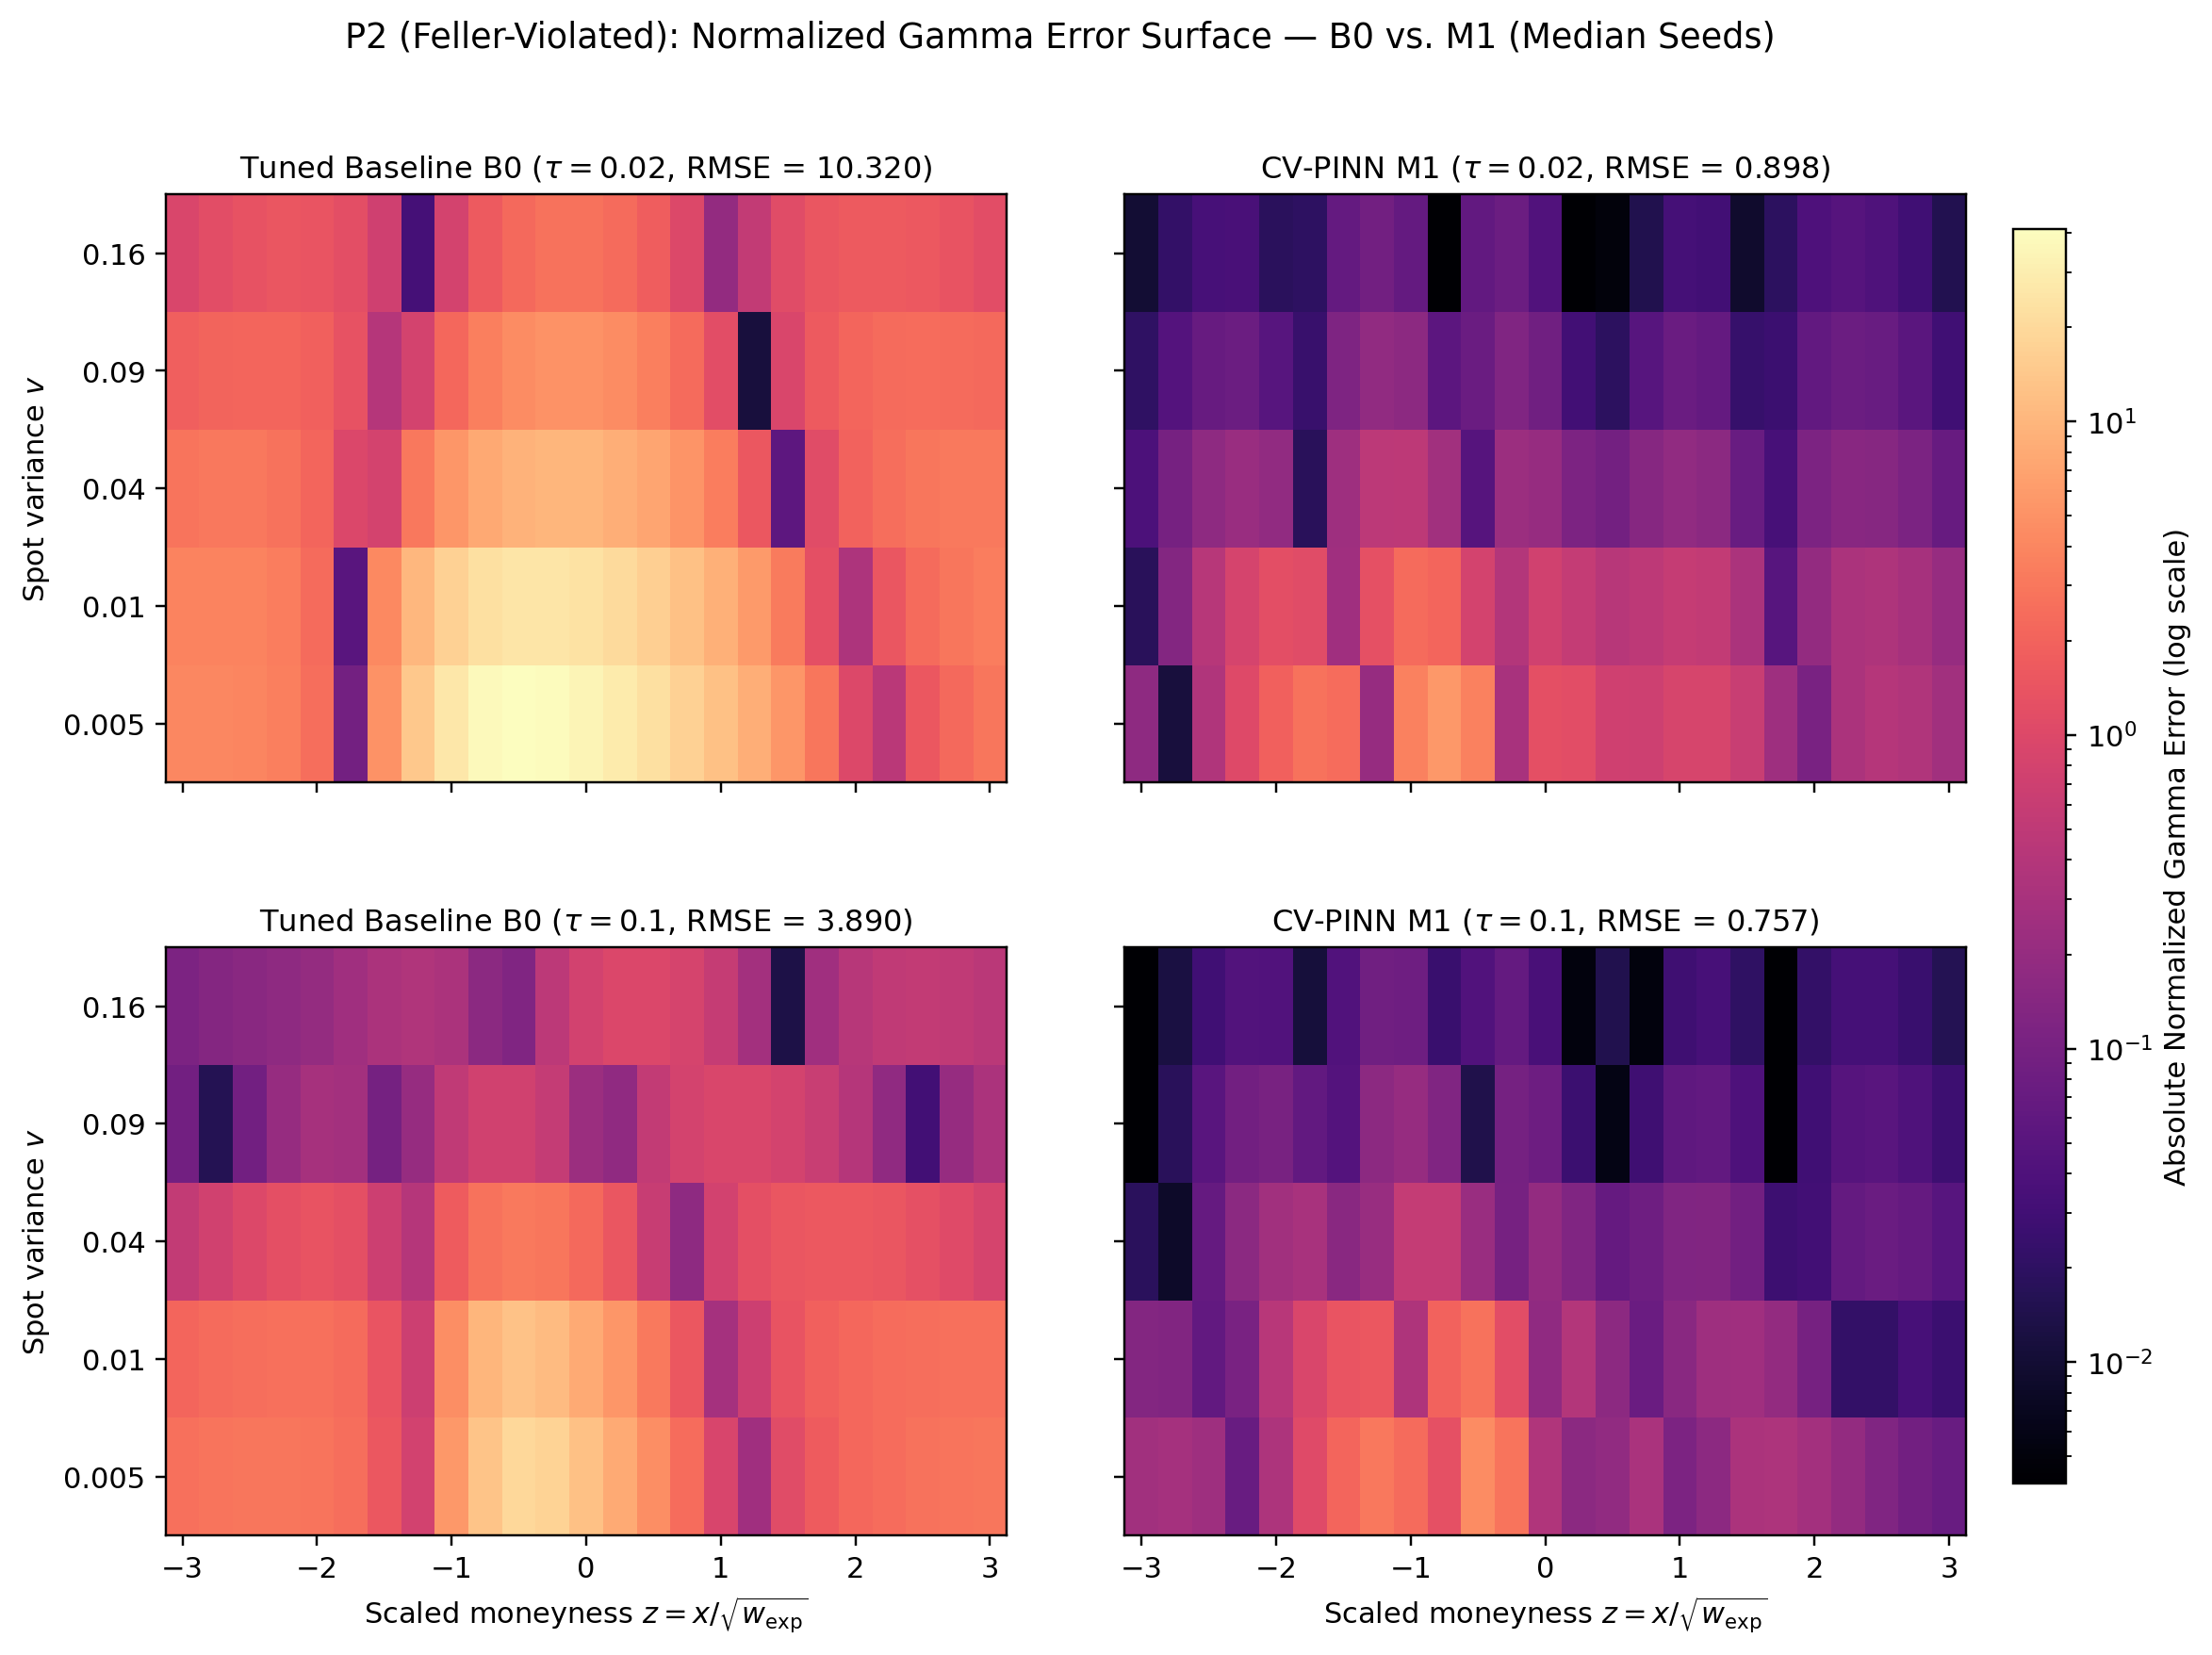
\includegraphics[width=0.49\textwidth]{fig1_gamma_error_surface_p2.png}\hfill
  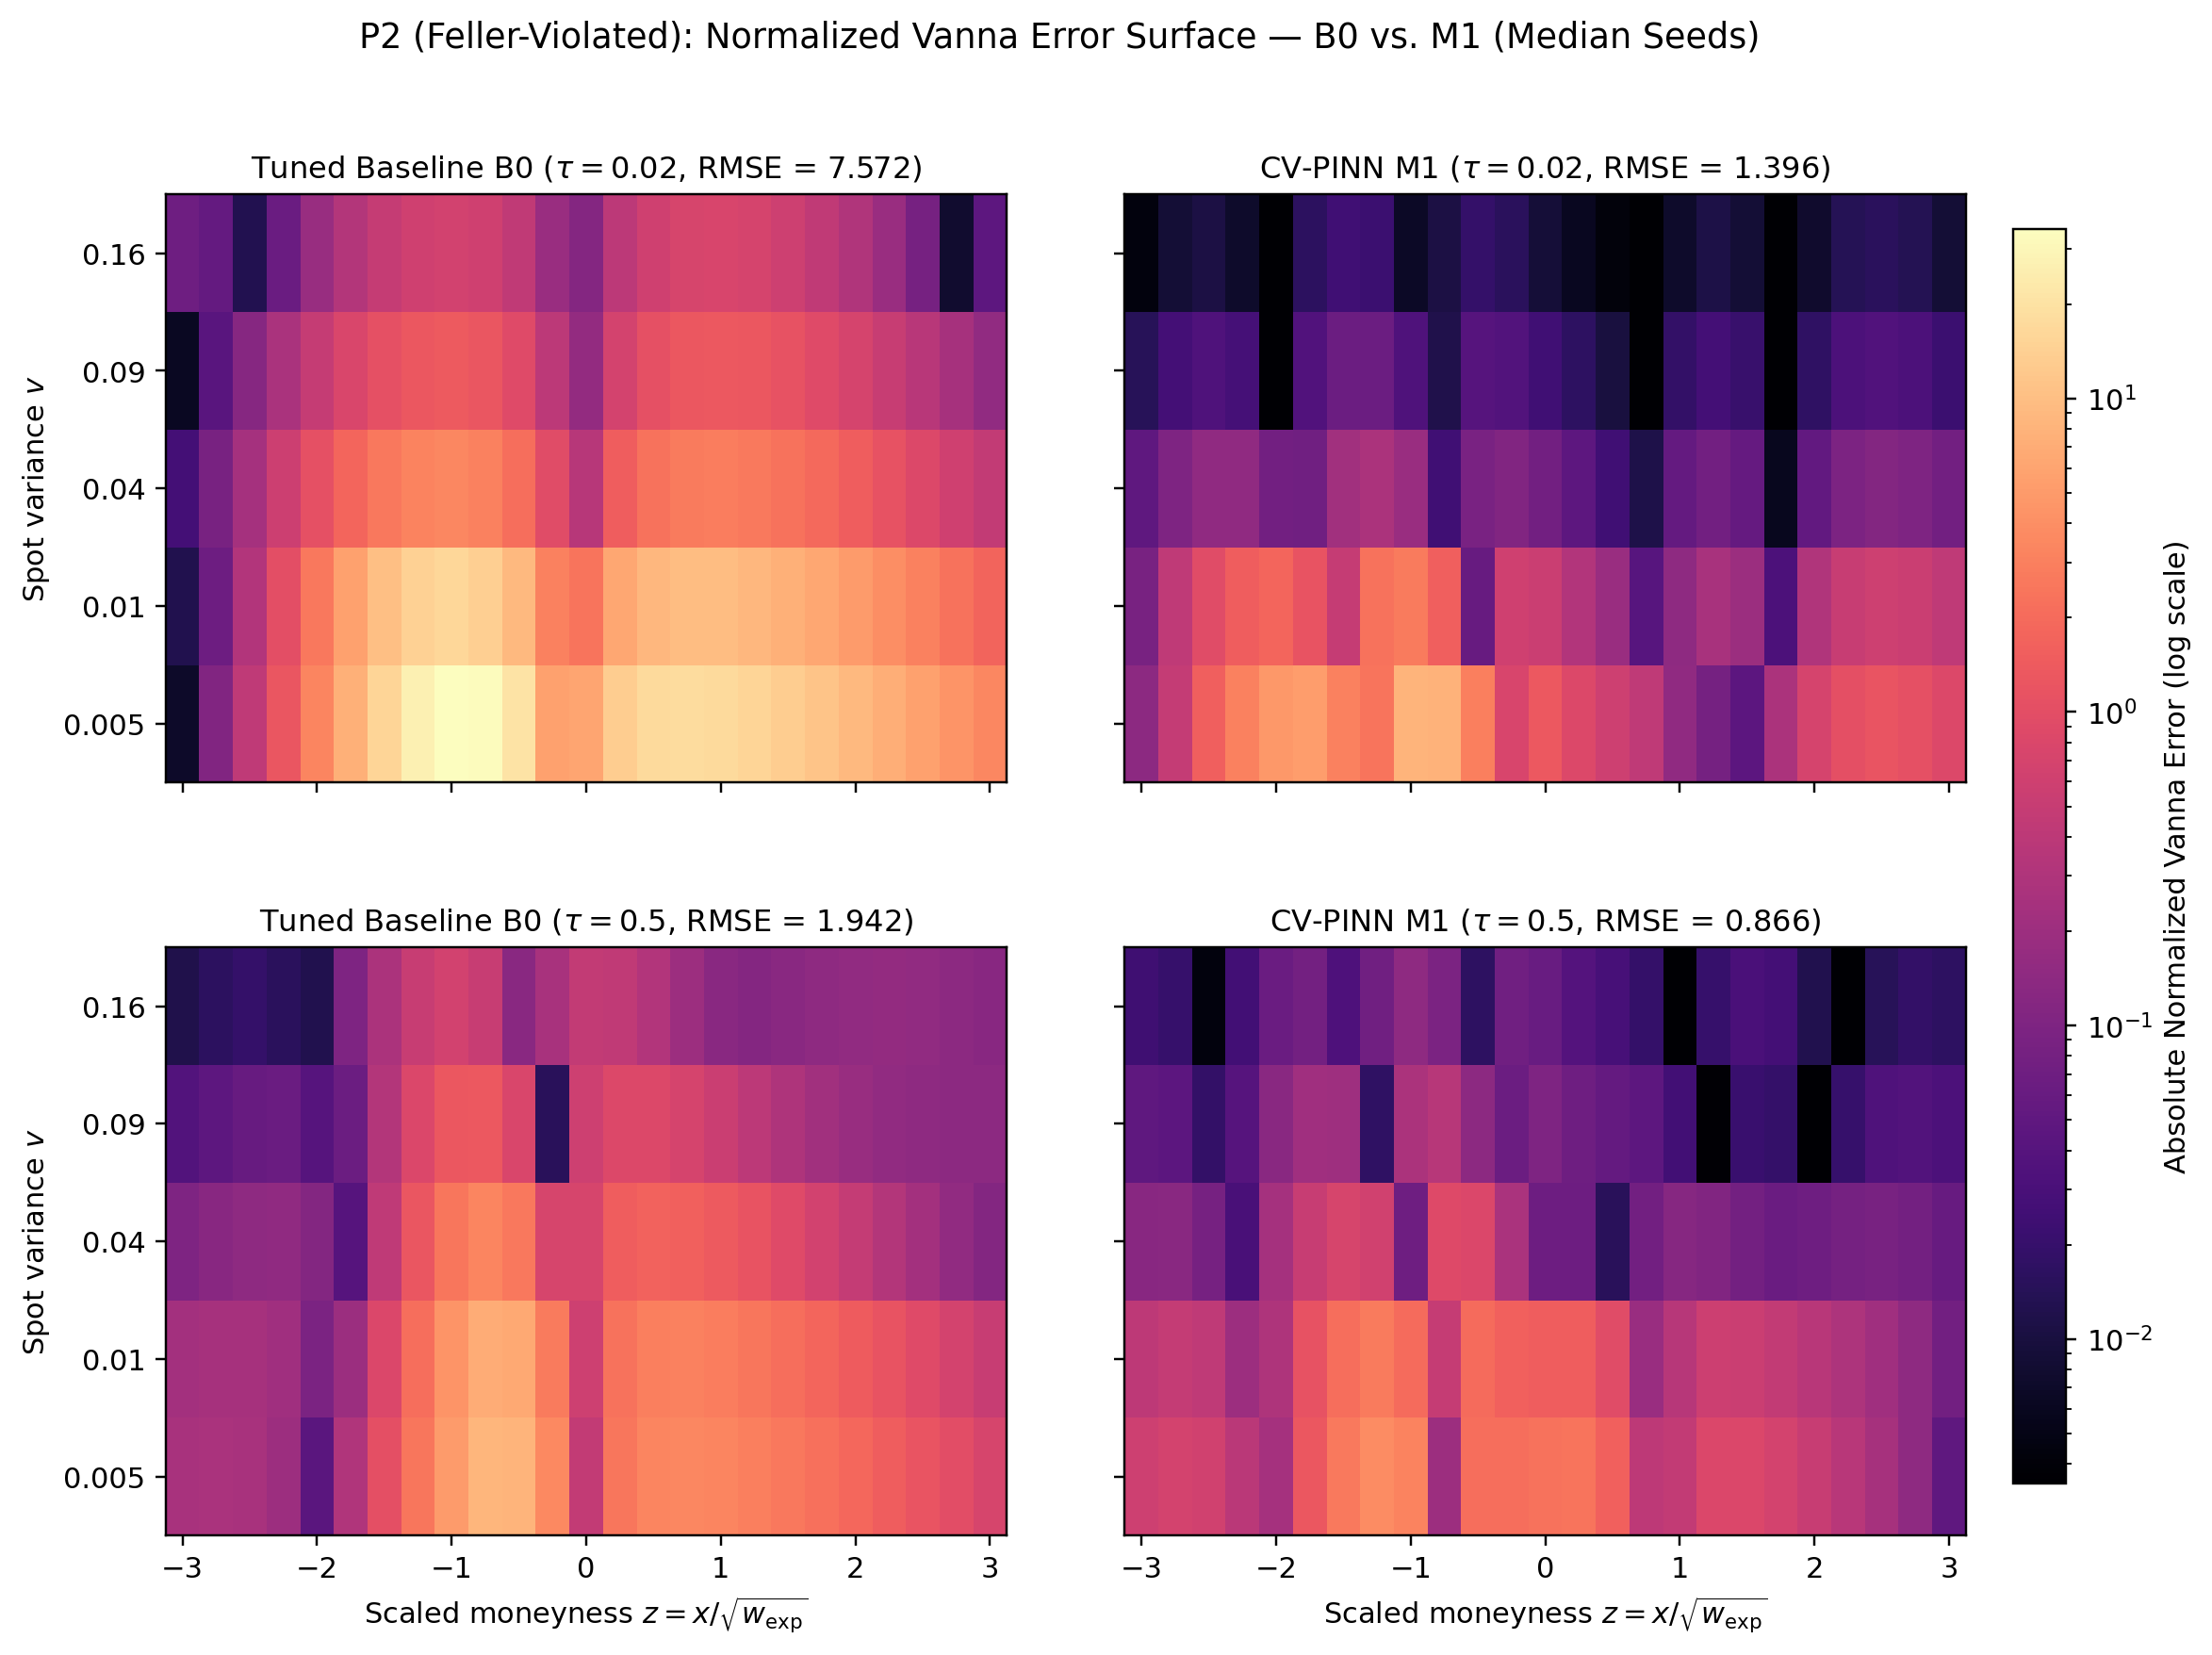
\includegraphics[width=0.49\textwidth]{fig2_vanna_error_surface_p2.png}
  \caption{Near-expiry ($\tau = 0.05$) absolute Gamma (left) and Vanna (right) error surfaces on Feller-violating \texttt{P2} comparing tuned baseline \texttt{B0} against expected-variance \texttt{M1} (median seeds).}
  \label{fig:p2_surfaces}
\end{figure}

\begin{figure}[htbp]
  \centering
  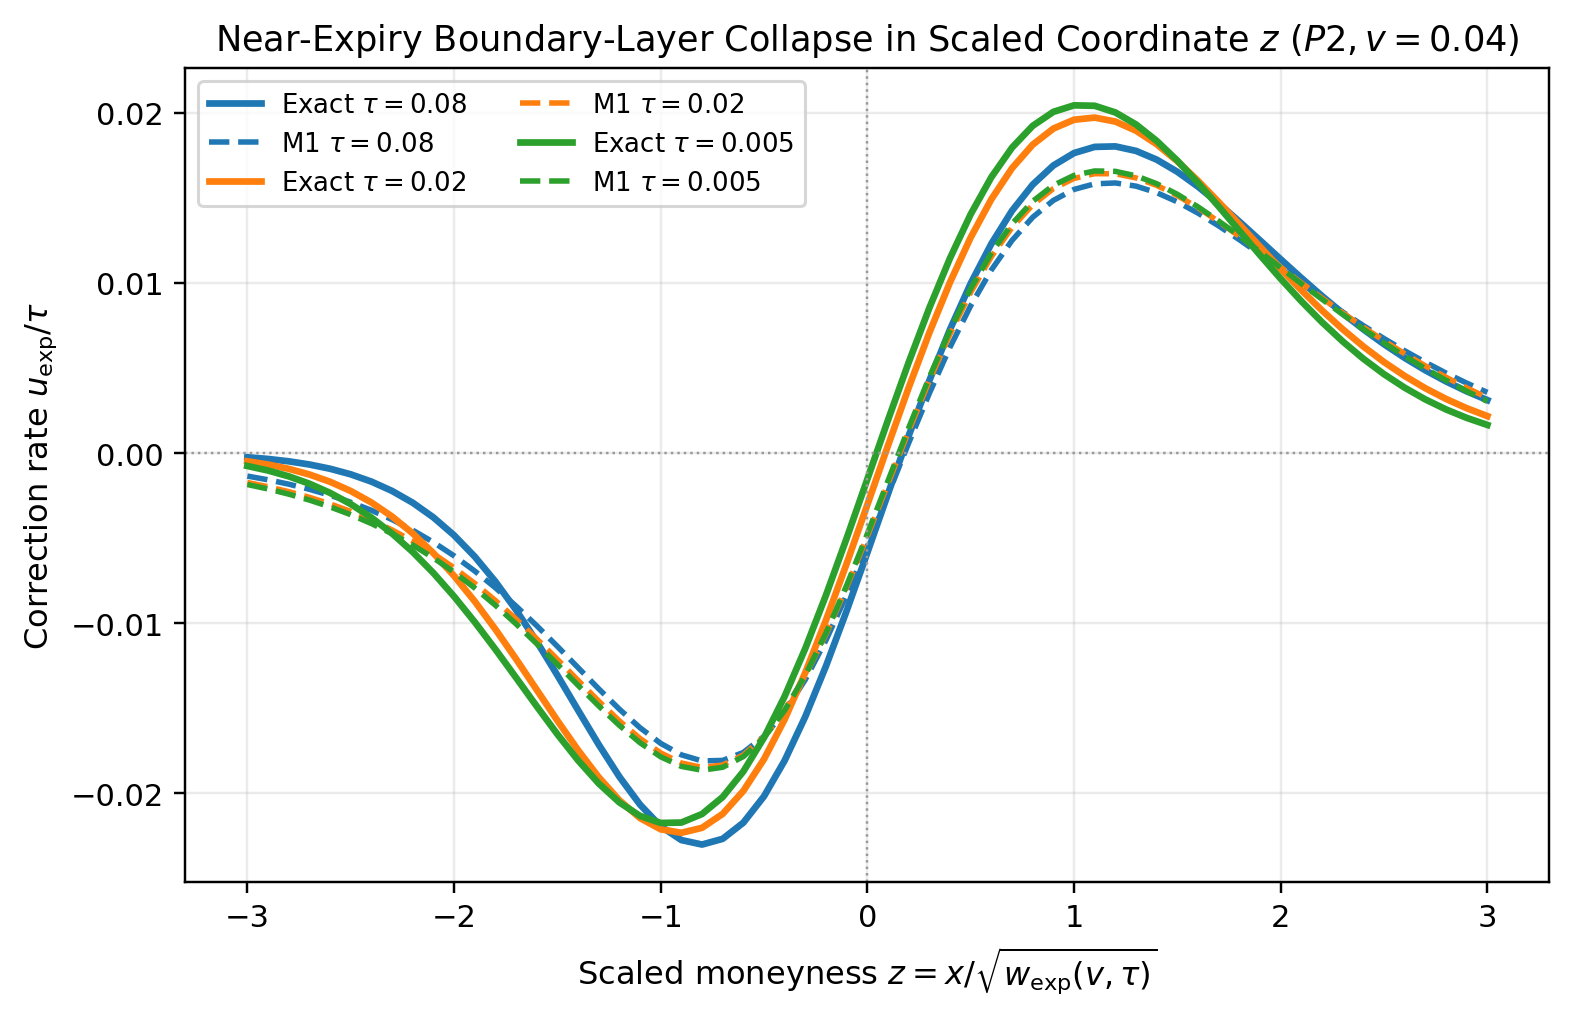
\includegraphics[width=0.49\textwidth]{fig3_boundary_layer_collapse.png}\hfill
  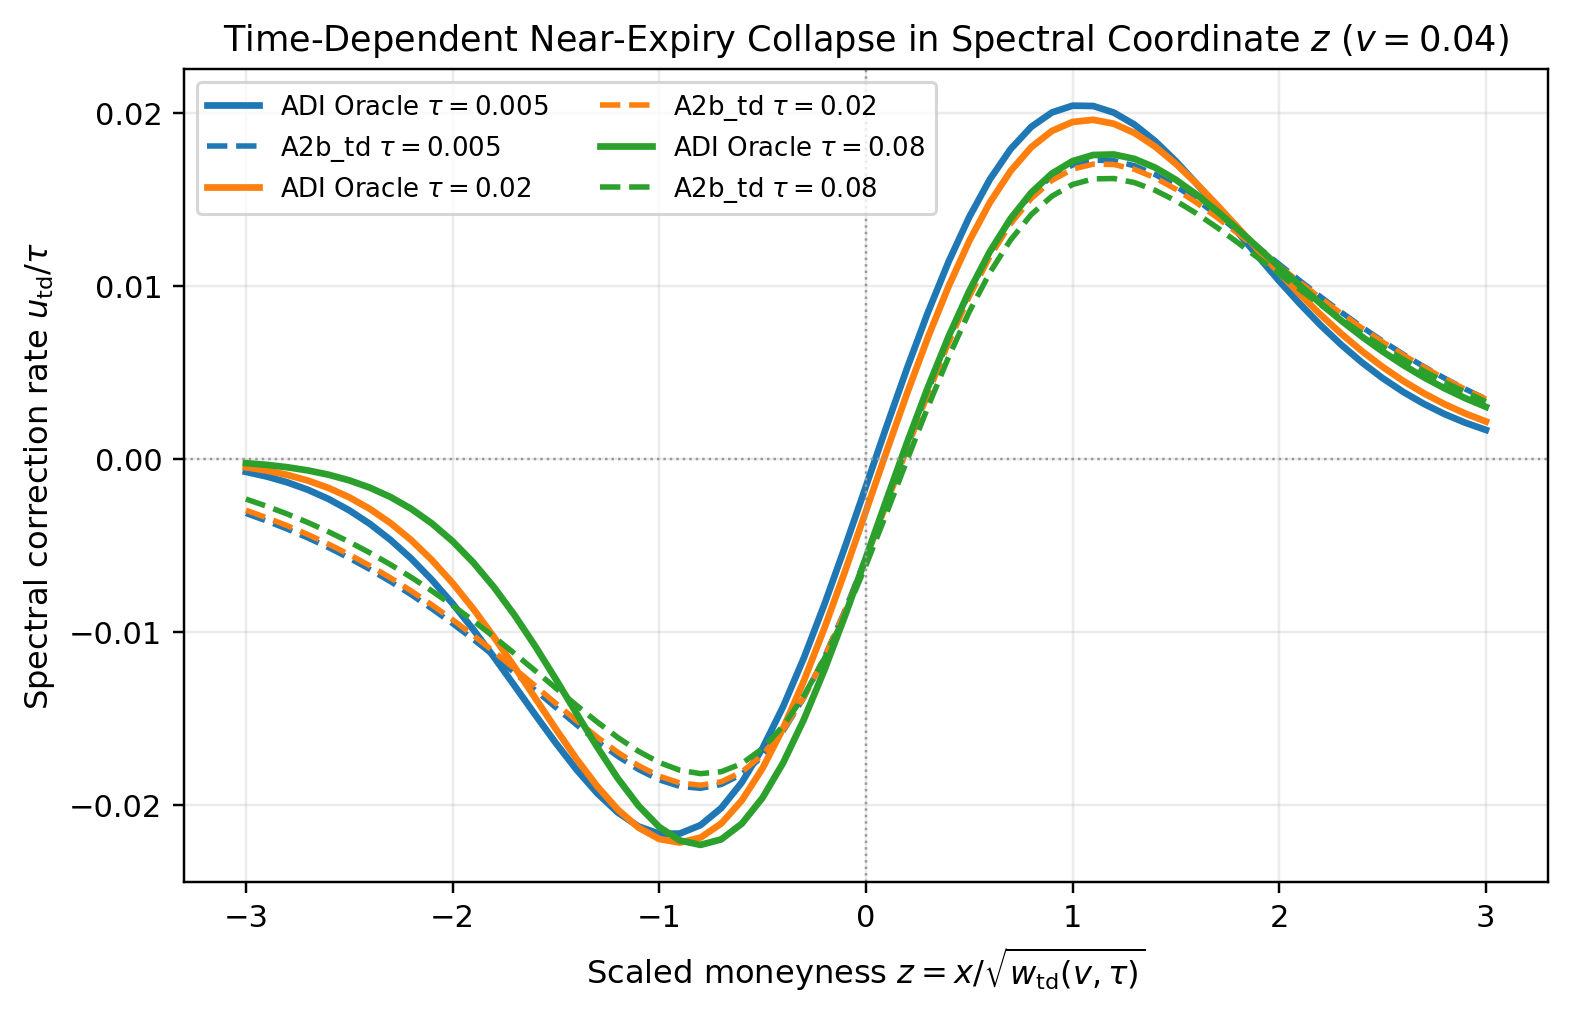
\includegraphics[width=0.49\textwidth]{fig6_td_boundary_layer_collapse.png}
  \caption{Self-similar collapse of the learned near-expiry correction rate $u_\phi/\tau$ along scaled moneyness $z = x/\sqrt{w}$ across $\tau \in \{0.08, 0.02, 0.005\}$ for constant-parameter \texttt{P2} (left) and spectral time-dependent \texttt{TD} (right).}
  \label{fig:bl_collapse}
\end{figure}

\begin{figure}[htbp]
  \centering
  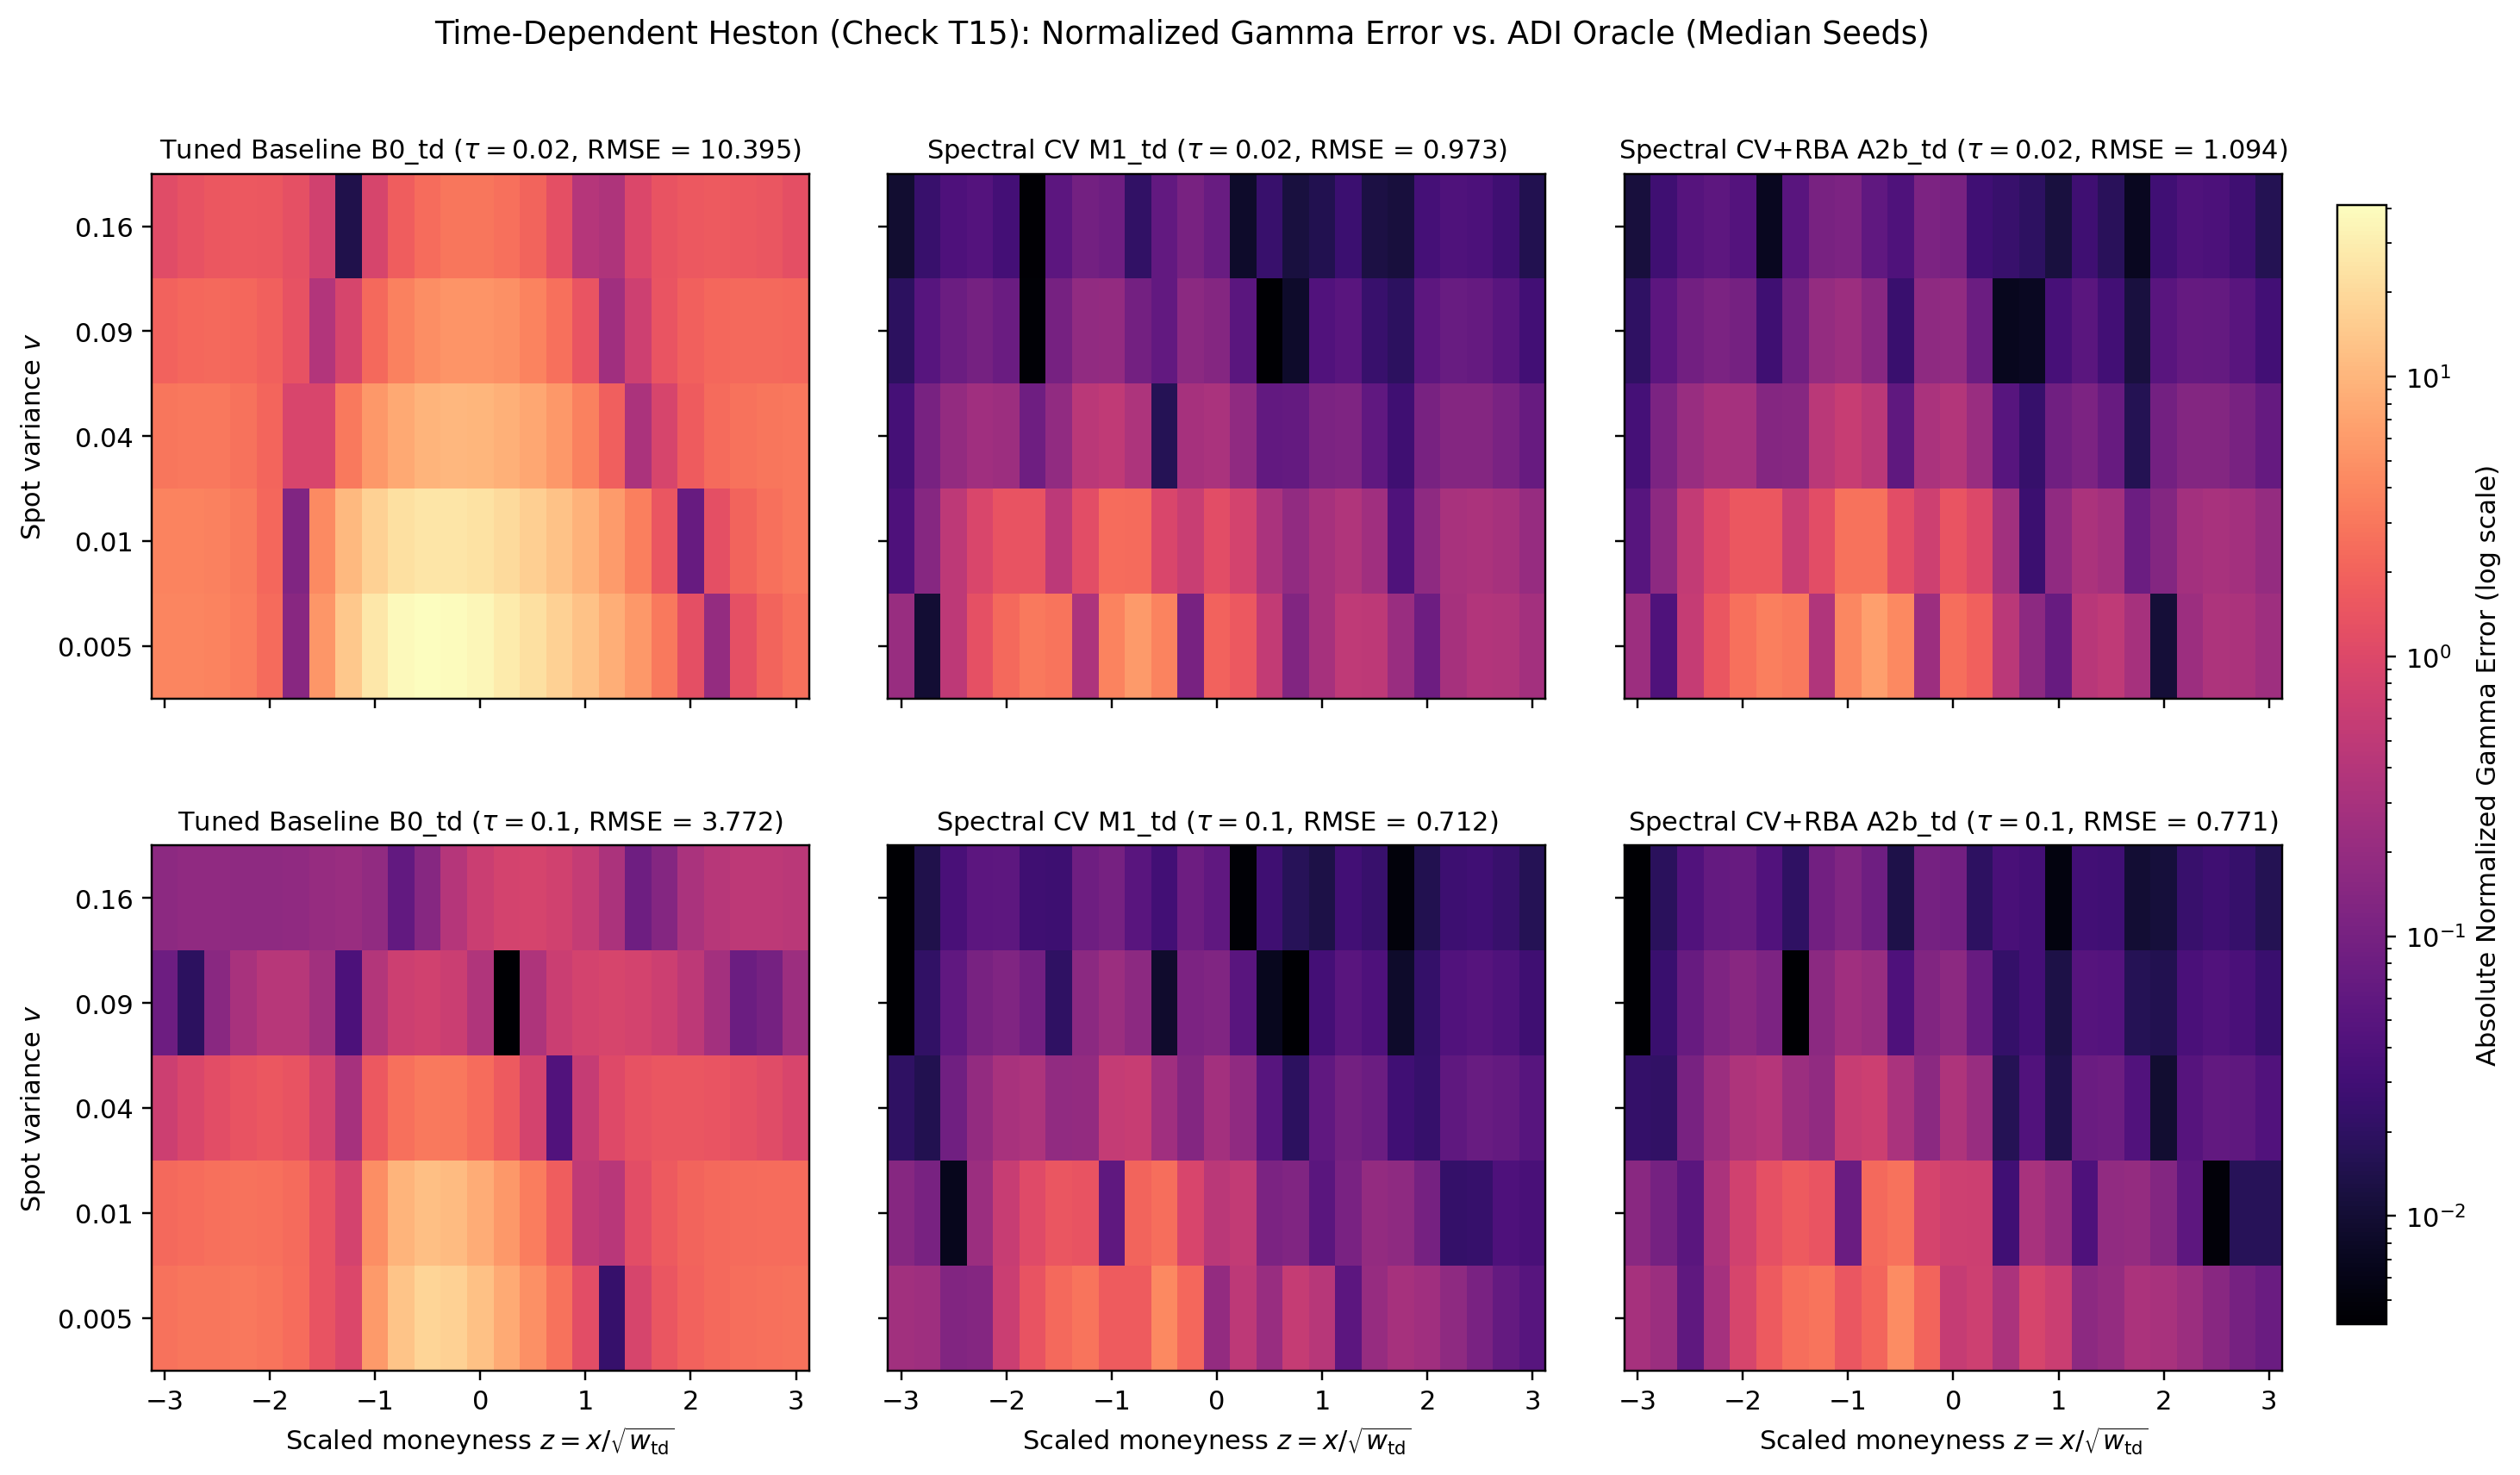
\includegraphics[width=0.49\textwidth]{fig4_td_gamma_error_surface.png}\hfill
  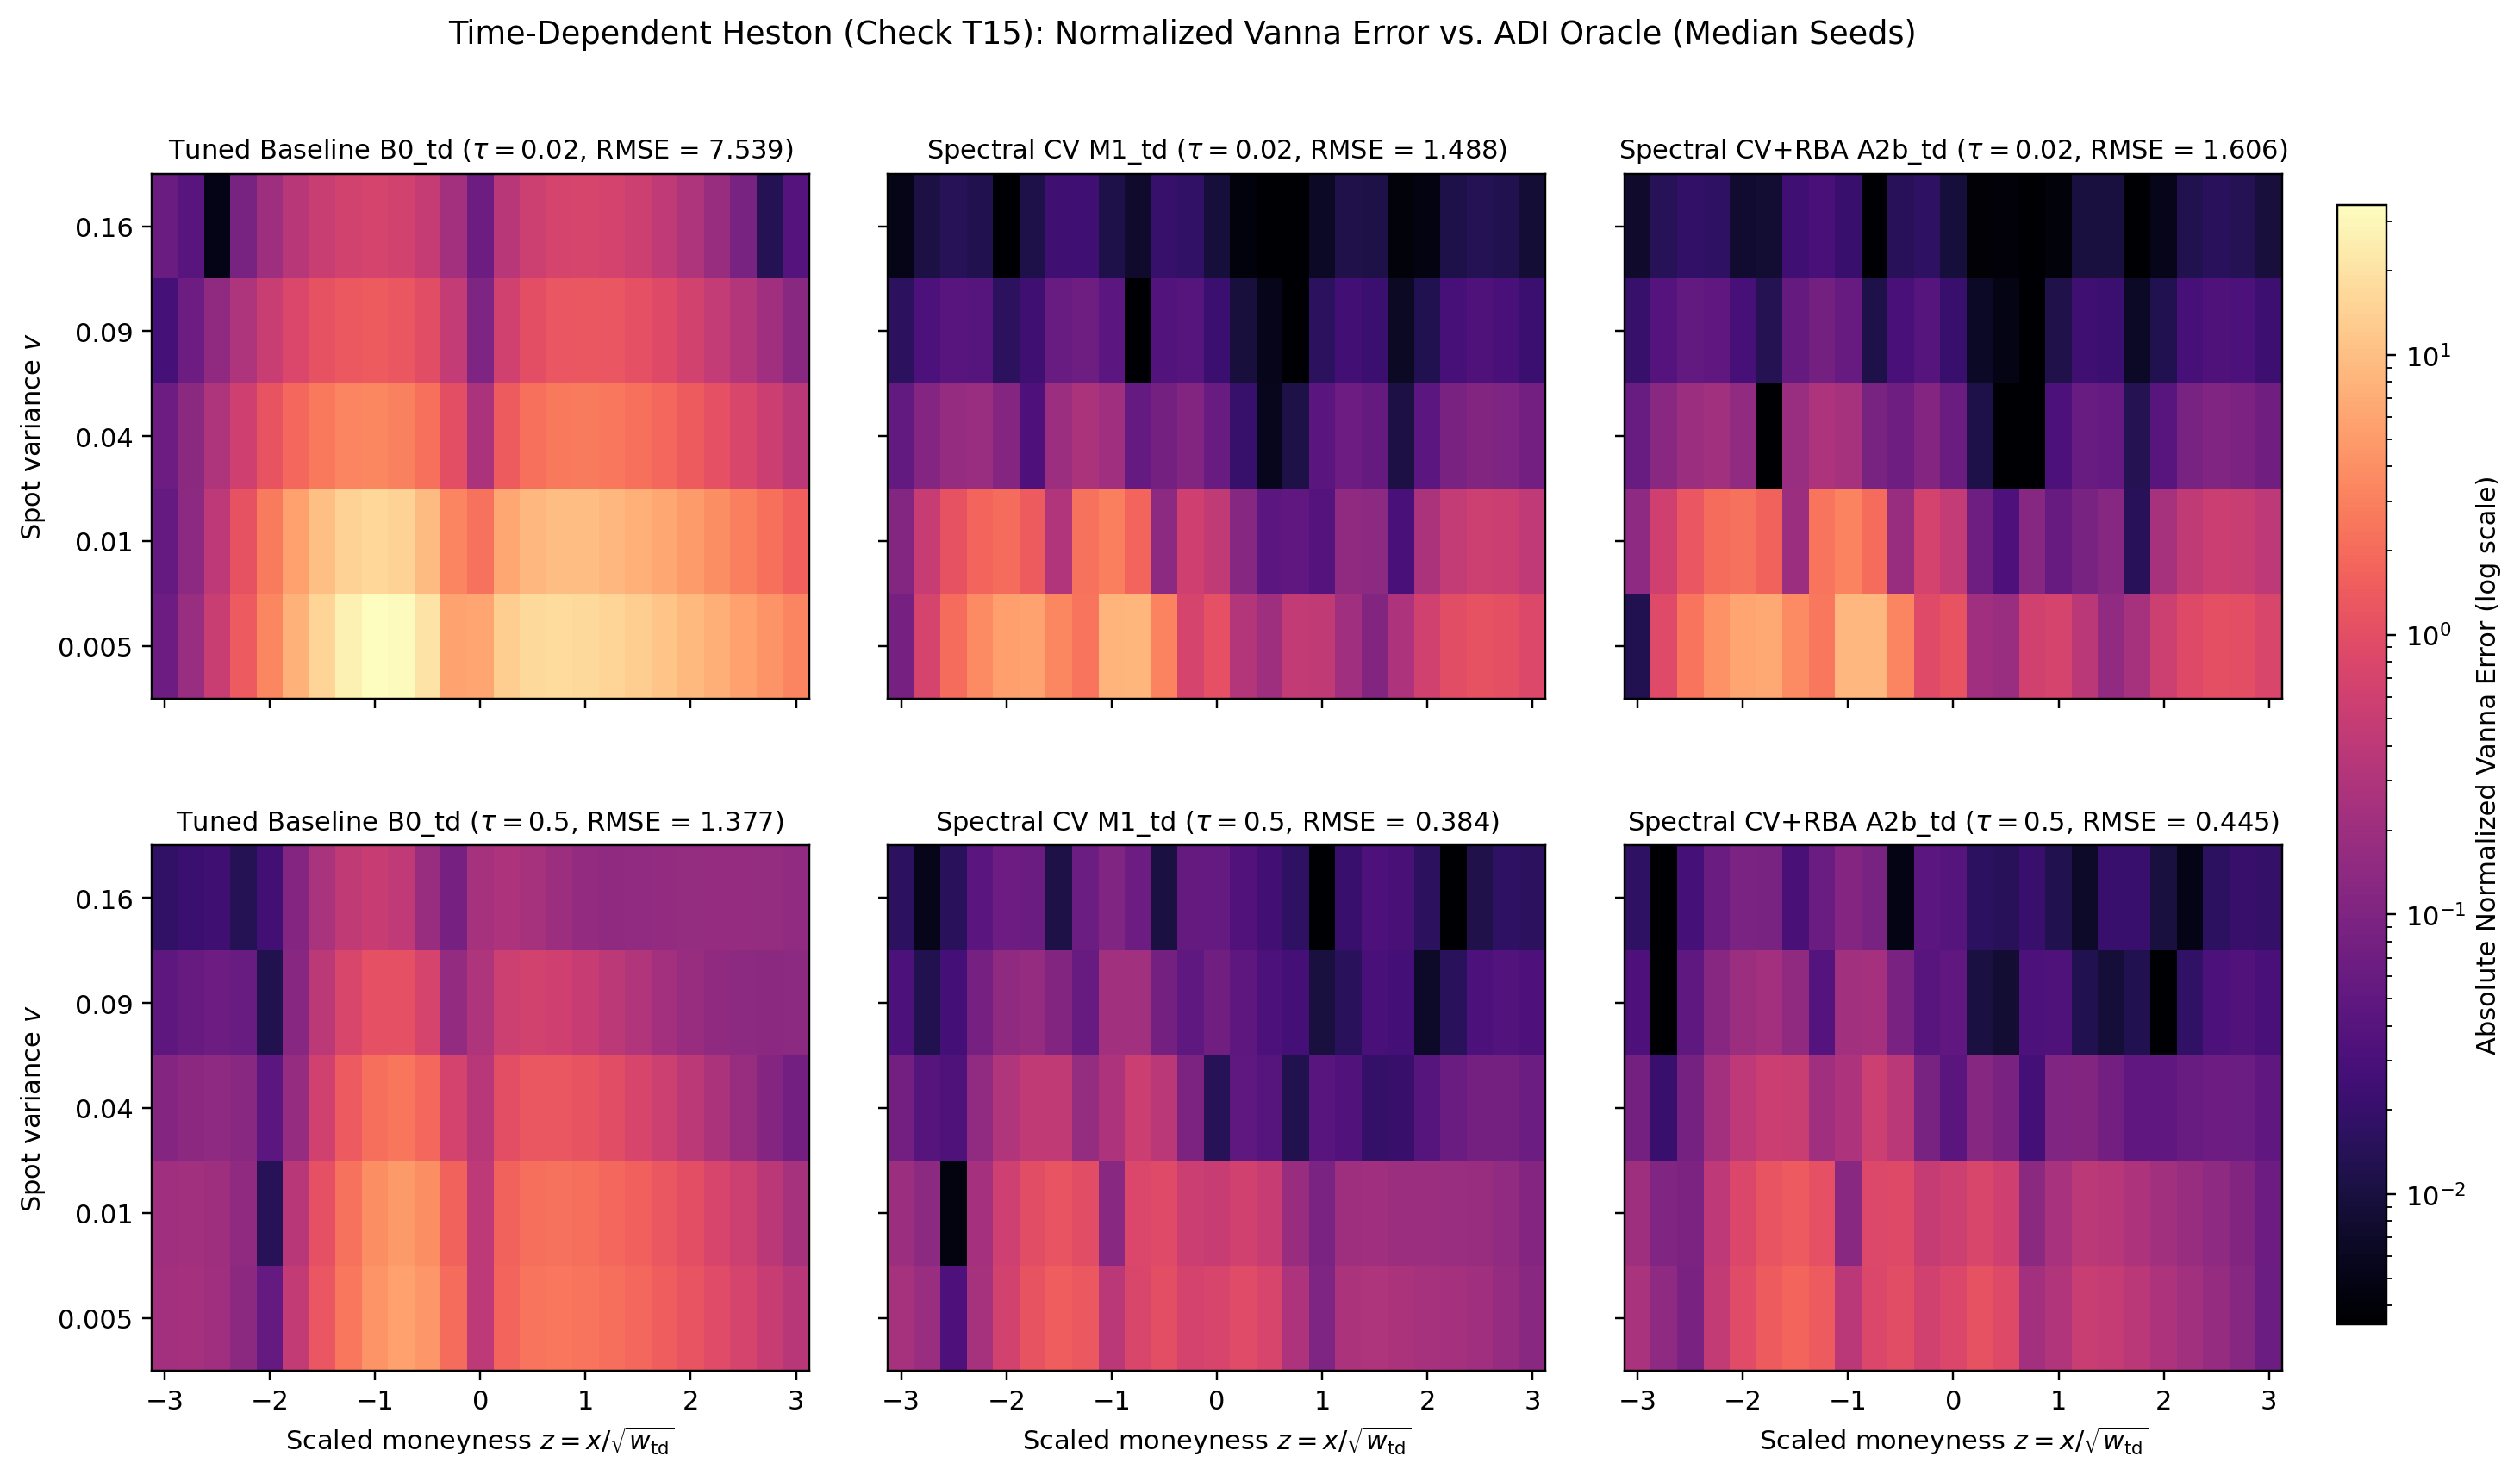
\includegraphics[width=0.49\textwidth]{fig5_td_vanna_error_surface.png}
  \caption{Time-dependent Heston (\texttt{T15}) absolute Gamma (left) and Vanna (right) error surfaces at $\tau = 0.05$ against the fine 2D ADI oracle across \texttt{B0\_td}, \texttt{M1\_td}, and energy-locked \texttt{A2b\_td}.}
  \label{fig:td_surfaces}
\end{figure}

\begin{figure}[htbp]
  \centering
  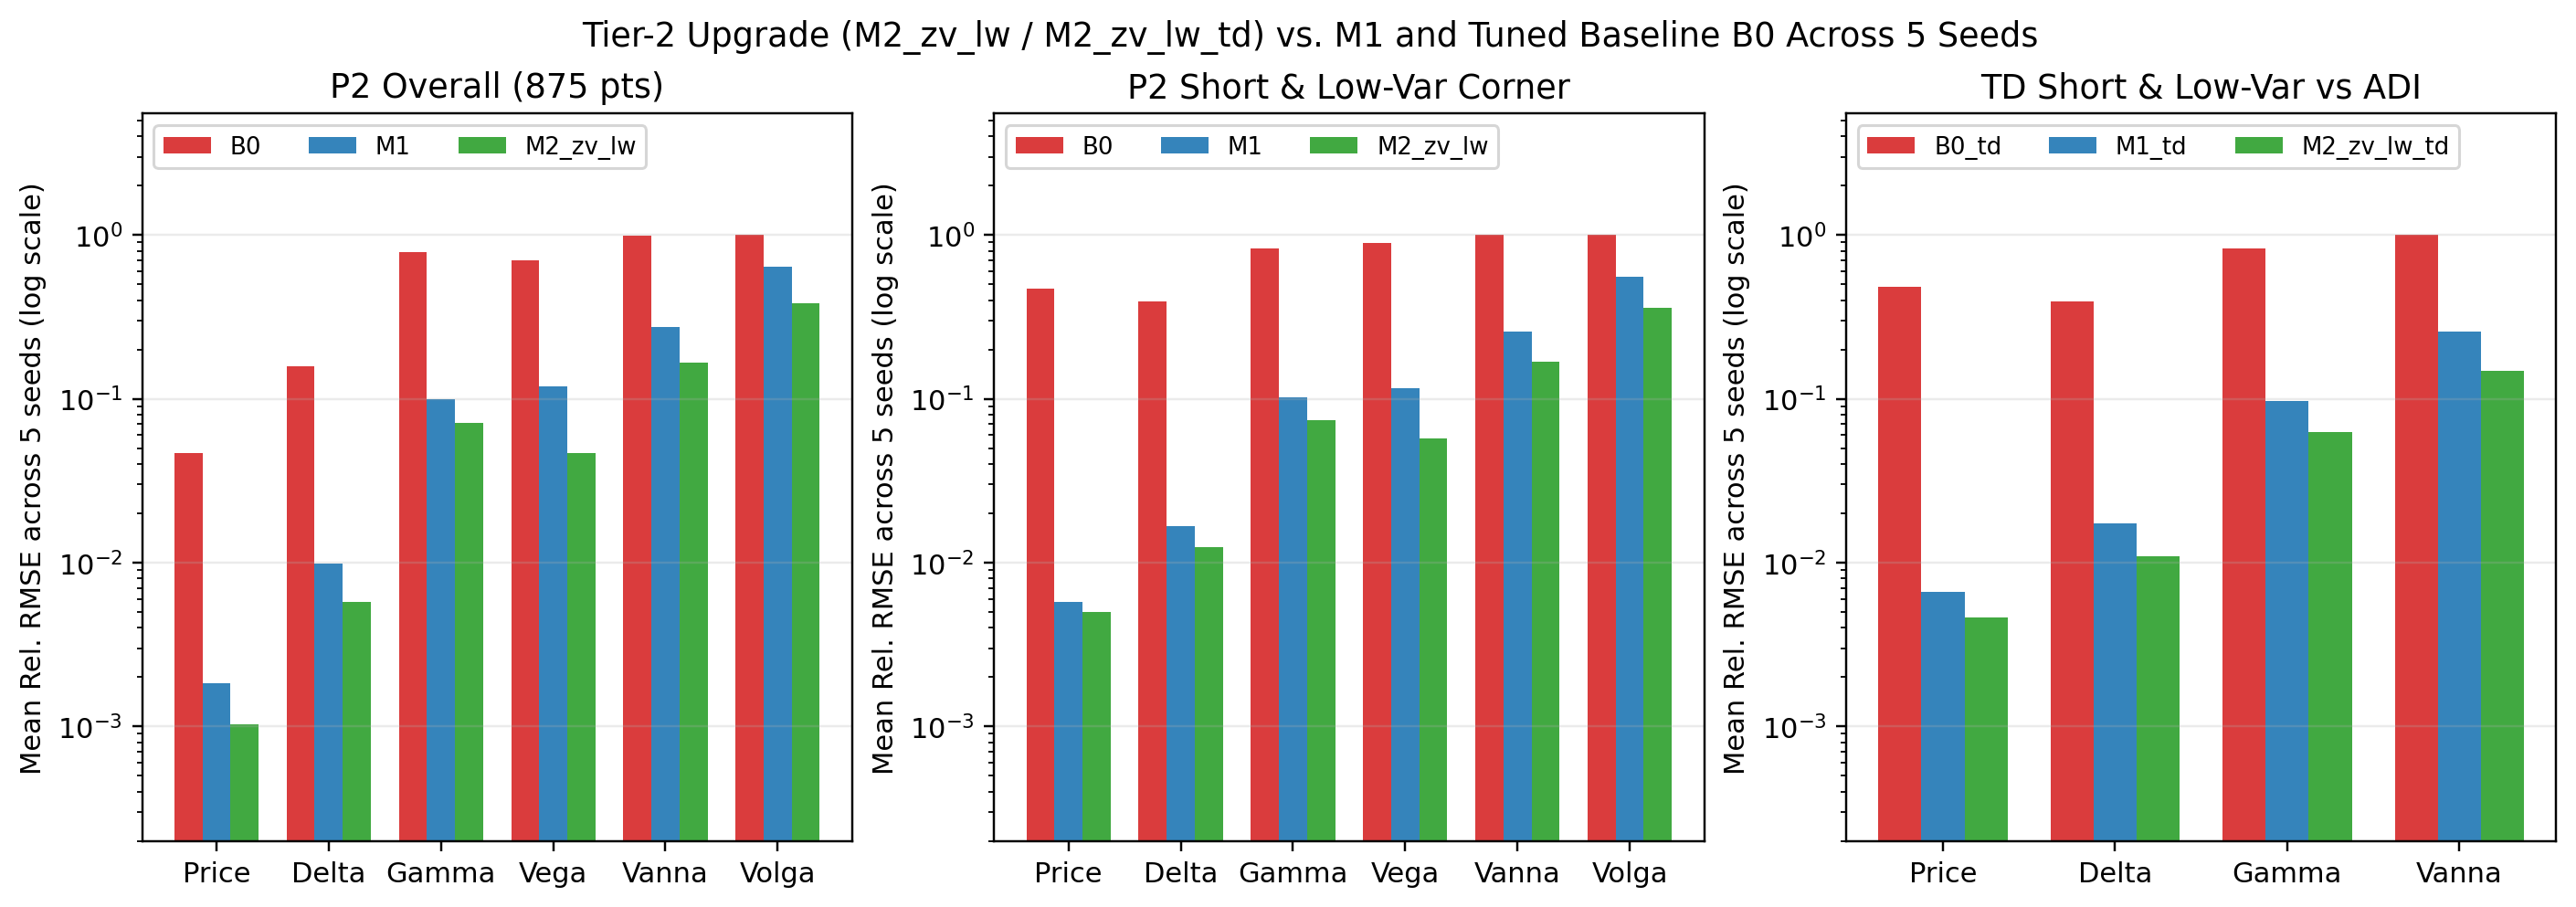
\includegraphics[width=0.92\textwidth]{fig7_tier2_accuracy_comparison.png}
  \caption{Tier-2 boundary-layer upgrade (\texttt{M2\_zv\_lw} / \texttt{M2\_zv\_lw\_td}) vs.\ \texttt{M1} and \texttt{B0} across all six outputs on \texttt{P1}, \texttt{P2}, and \texttt{TD}.}
  \label{fig:tier2_comp}
\end{figure}

\begin{figure}[htbp]
  \centering
  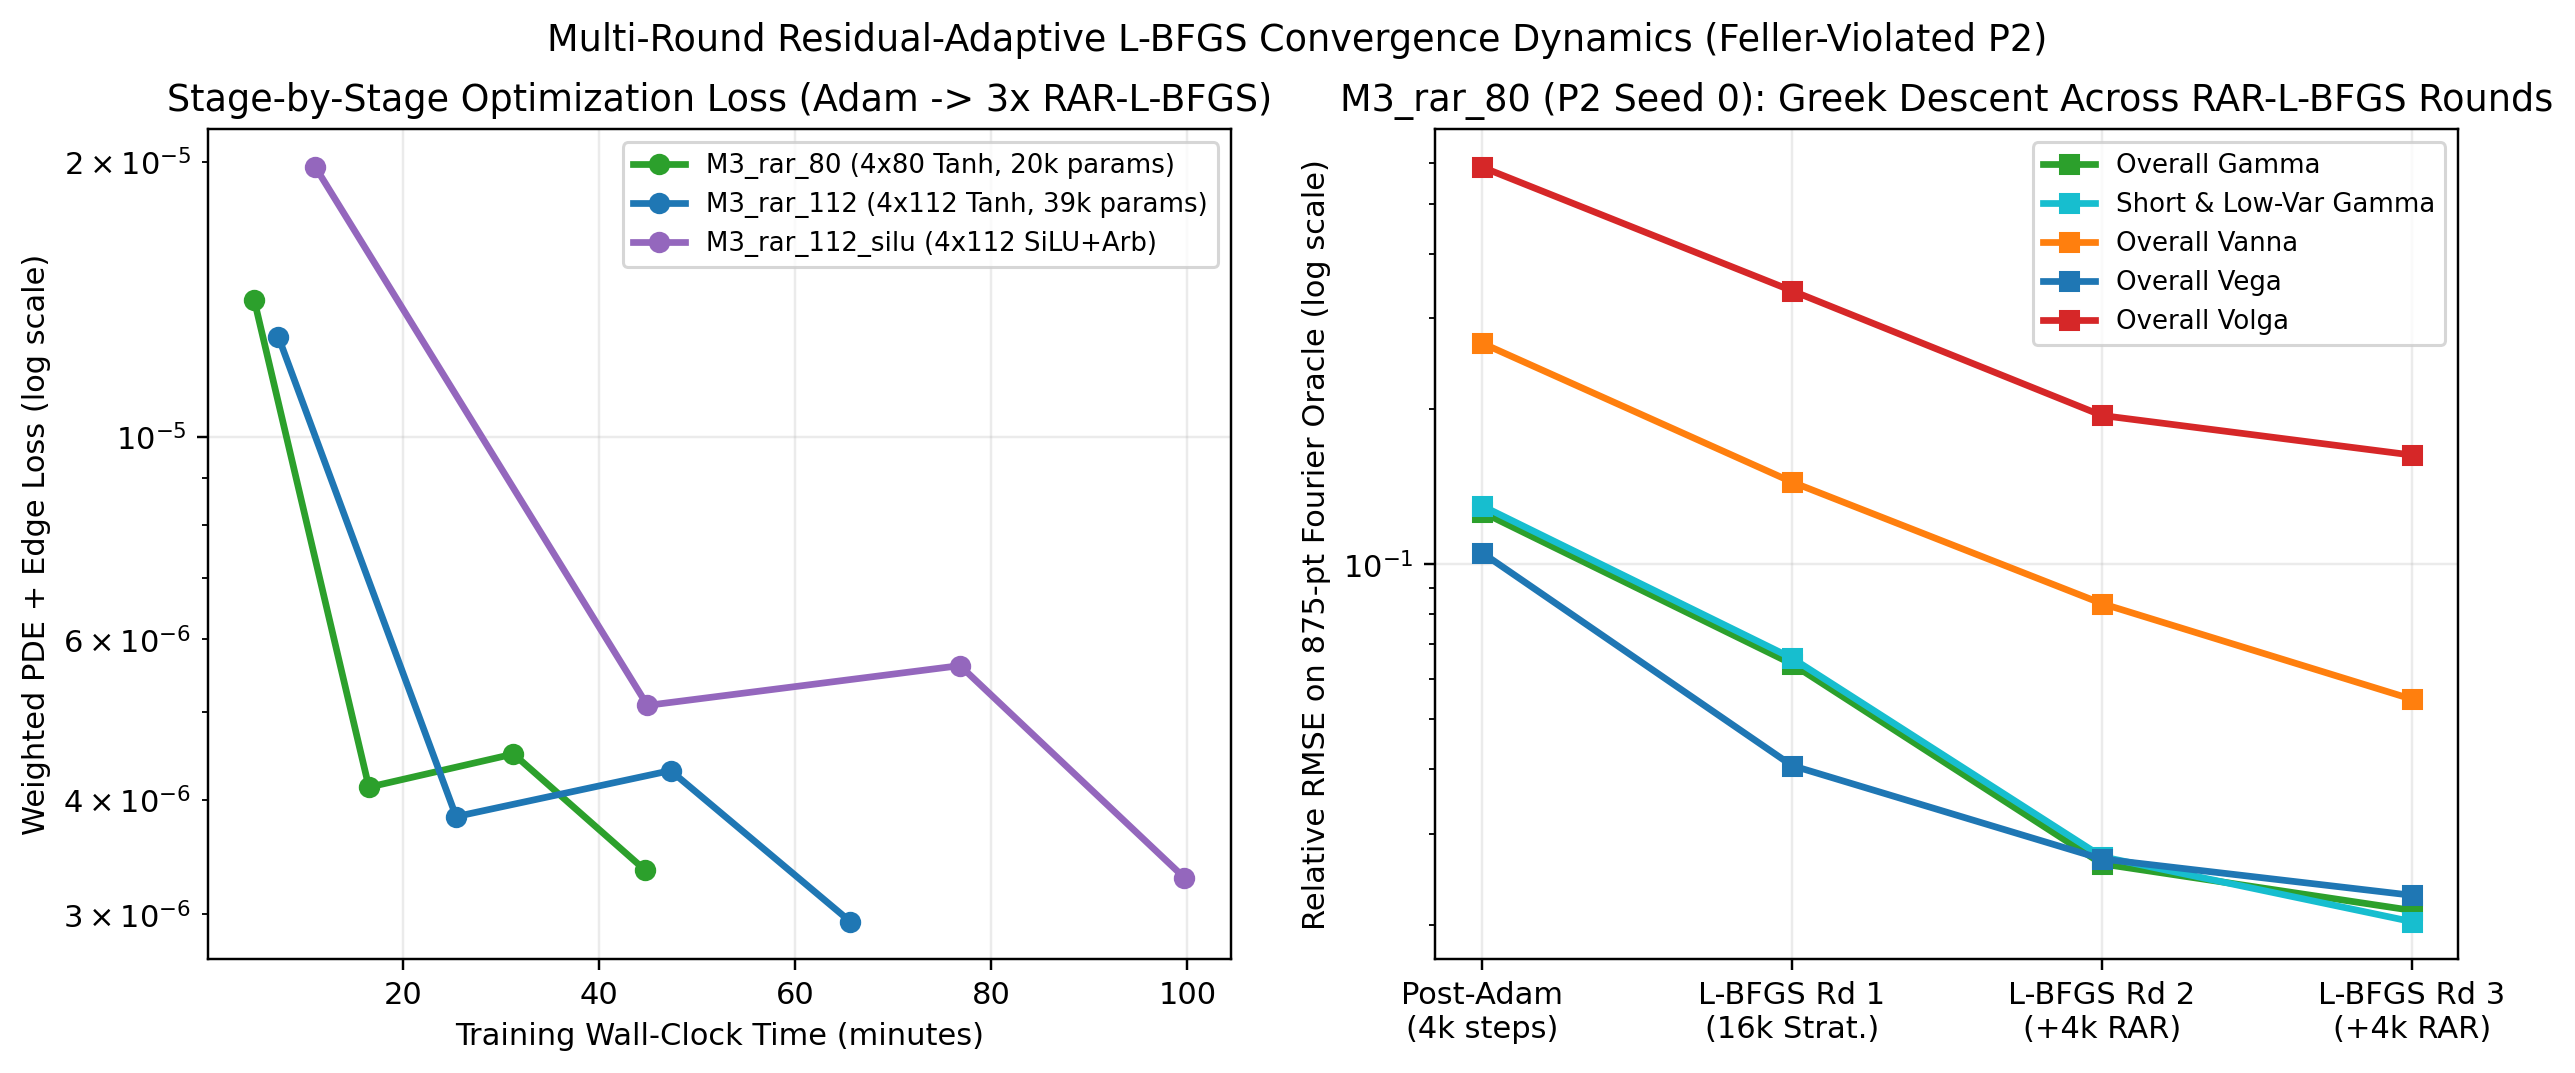
\includegraphics[width=0.95\textwidth]{fig9_m3_convergence_trajectories.png}
  \caption{Optimization and Greek error trajectories of \texttt{M3\_rar\_80} across $4{,}000$ Adam warm-up steps and three $1{,}200$-iteration Strong-Wolfe \texttt{RAR-L-BFGS} rounds.}
  \label{fig:m3_conv}
\end{figure}

\begin{figure}[htbp]
  \centering
  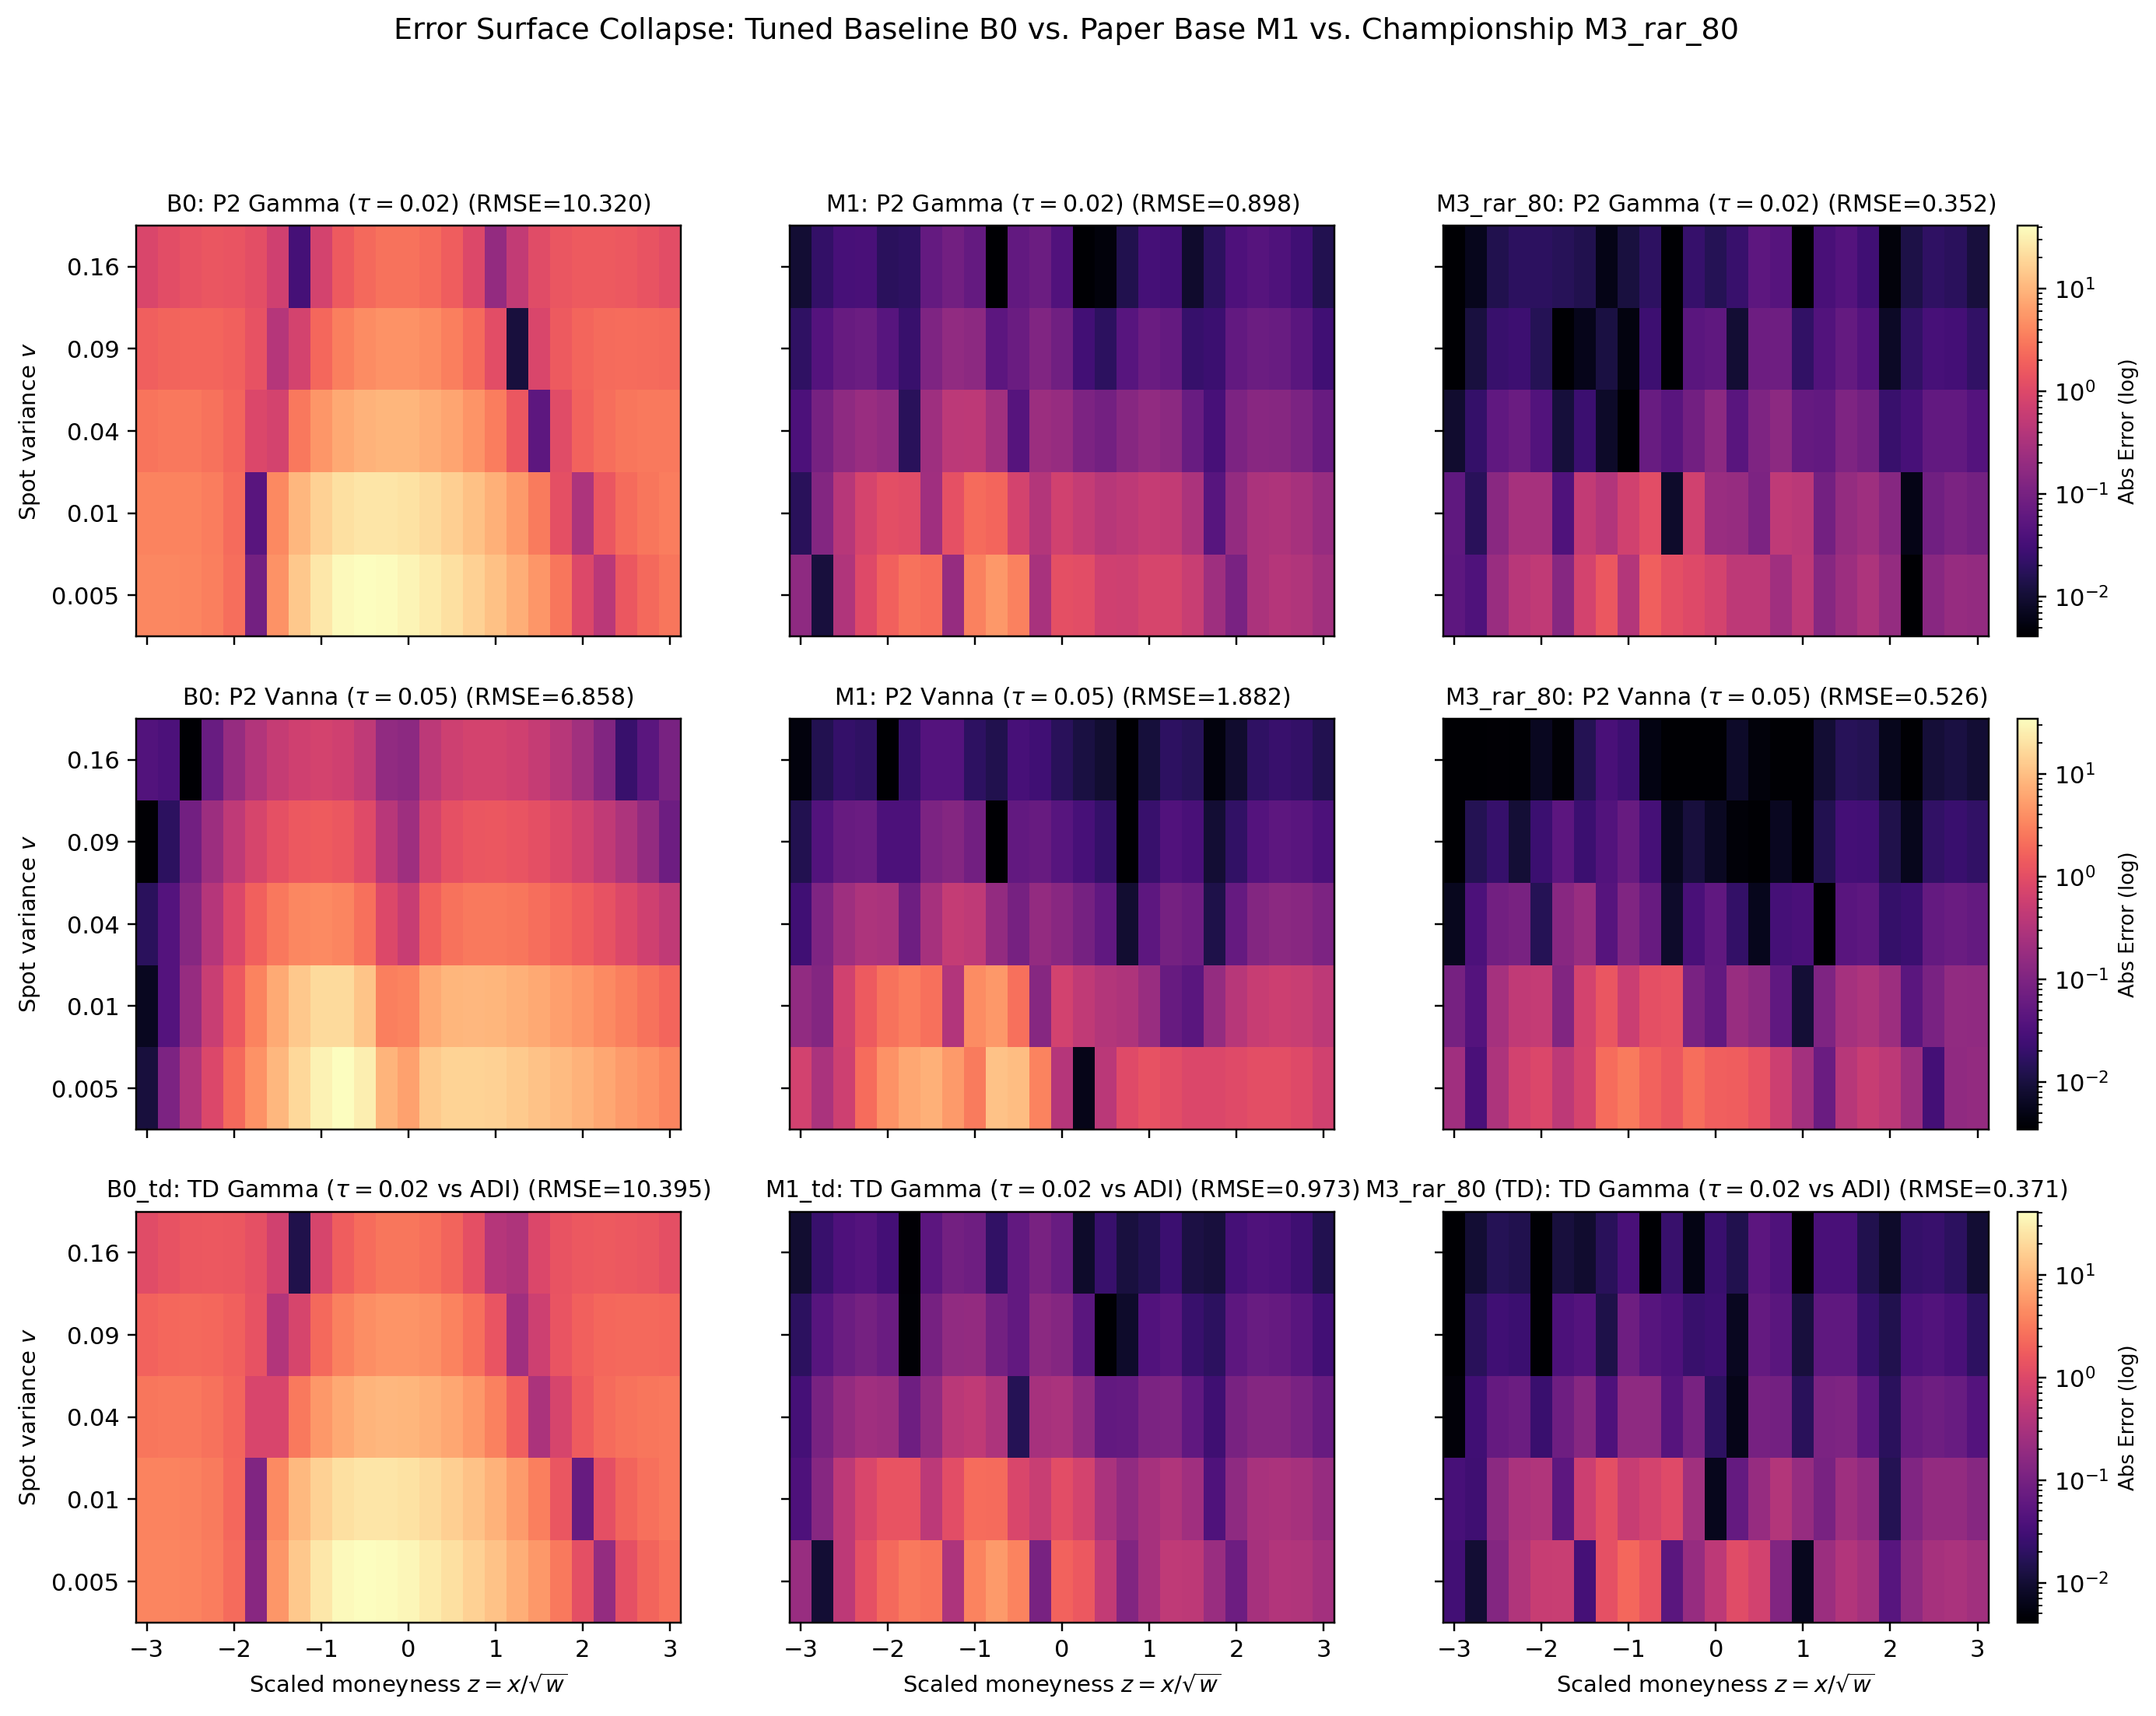
\includegraphics[width=0.95\textwidth]{fig10_m3_error_surfaces_p2_and_td.png}
  \caption{Progressive collapse of near-expiry Gamma error surfaces across \texttt{B0} $\to$ \texttt{M1} $\to$ championship \texttt{M3\_rar\_80} on Feller-violating \texttt{P2} and time-dependent \texttt{TD}.}
  \label{fig:m3_surfaces}
\end{figure}

\begin{figure}[htbp]
  \centering
  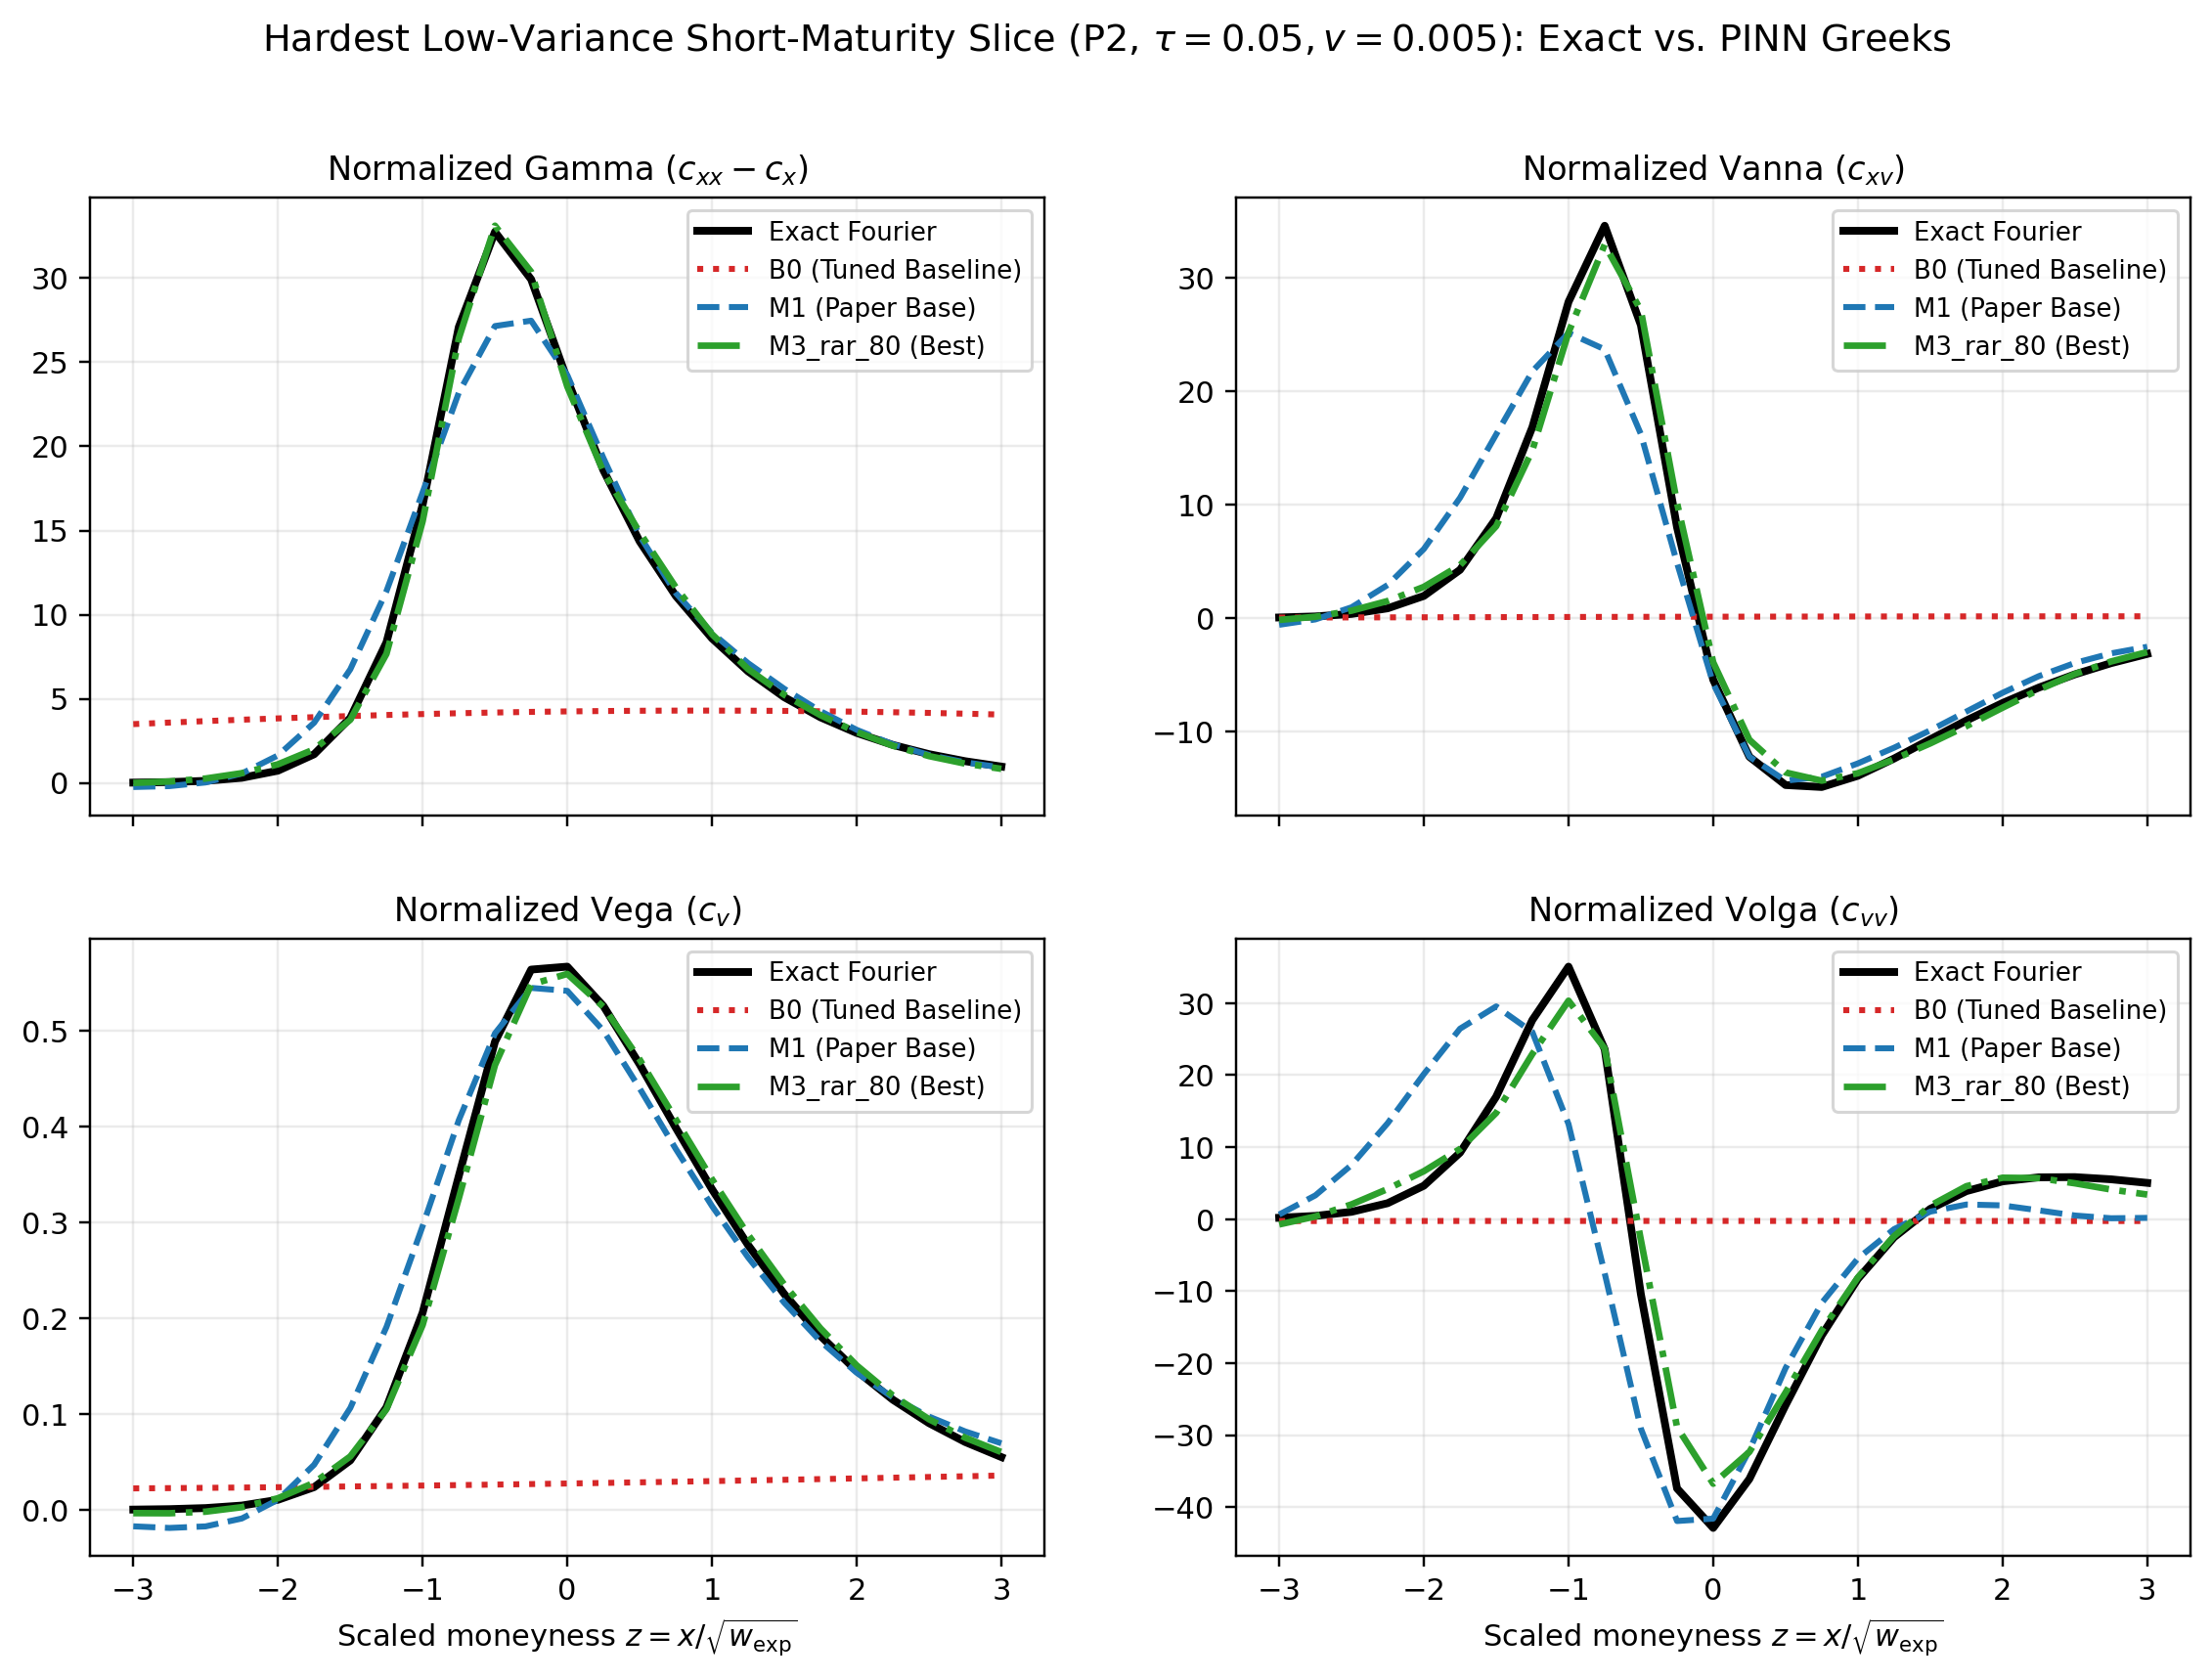
\includegraphics[width=0.95\textwidth]{fig11_hardest_slice_profiles.png}
  \caption{Exact Fourier vs.\ \texttt{B0}, \texttt{M1}, and \texttt{M3\_rar\_80} 1D Greek profiles (Gamma, Vanna, Vega, Volga) on the single hardest Feller-violating boundary slice ($\tau = 0.05, v = 0.005$ on \texttt{P2}).}
  \label{fig:slice_profiles}
\end{figure}

\subsection{Mechanistic Ablations, No-Arbitrage Admissibility, and Wing Decay}

Table~\ref{tab:arb} and Figure~\ref{fig:ladder} dissect each architectural component and audit static no-arbitrage admissibility on Feller-violated \texttt{P2}. Removing the Gaussian variance carrier while keeping hard terminal payoff enforcement (\texttt{A0\_intr}: $c = (e^x - 1)^+ + \tau N_\phi$) collapses completely ($1.0000$ relative RMSE across Gamma, Vanna, Vega, and Volga, with $89$ core negative-Gamma violations). Removing $\tanh(z/2)$ while keeping $b(x, w_{\mathrm{exp}})$ (\texttt{M1\_noz}) degrades Gamma nearly $10\times$ relative to \texttt{M3\_rar\_80} ($0.2571$ vs.\ $0.0273$). Across all 9 multi-seed runs on \texttt{P1}, \texttt{P2}, and \texttt{TD}, \texttt{M3\_rar\_80} achieves \textbf{zero negative-Gamma violations inside the liquid core $|z| \le 2$}. Remaining sign flips occur solely in far wings $|z| \ge 2.25$ where true Gamma is $< 10^{-3}$; introducing the structural Lee-moment envelope $\mathcal{E}_{0.35}(z) = \operatorname{sech}(0.35 z)$ (\texttt{M3\_sech\_80}) damps far-wing overshoot structurally without slowing \texttt{L-BFGS} convergence as soft arbitrage penalties (\texttt{M3\_rar\_112\_arb}) do.

\begin{table}[htbp]
\centering
\caption{Mechanistic ablation ladder, static no-arbitrage audit, and tail error percentiles on Feller-violating \texttt{P2} (875 grid points).}
\label{tab:arb}
\footnotesize
\setlength{\tabcolsep}{4.5pt}
\resizebox{\textwidth}{!}{\begin{tabular}{lccccccc}
\toprule
Model / Ablation & Gamma Rel & Vanna Rel & Core Neg.\ $\Gamma$ ($|z|\le 2$) & Total Neg.\ $\Gamma$ & Worst $\min\Gamma$ & Floor Viol.\ & $\Gamma$ MAE / P95 / P99 \\
\midrule
\texttt{A0\_intr} (intrinsic only) & $1.0000$ & $1.0000$ & $89.0$ & $148.0$ & $-9.66\times 10^{-6}$ & $380.0$ & $2.837$ / $12.97$ / $29.61$ \\
\texttt{B0} (soft payoff PINN) & $0.7829$ & $0.9949$ & $13.0$ & $51.6$ & $-4.61\times 10^{-1}$ & $155.6$ & $1.975$ / $8.724$ / $25.20$ \\
\texttt{M1\_noz} (no $\tanh(z/2)$) & $0.2571$ & $0.4029$ & $6.0$ & $59.0$ & $-1.62\times 10^{-1}$ & $141.0$ & $0.657$ / $3.301$ / $6.945$ \\
\texttt{A1} (spot-var carrier) & $0.1584$ & $0.6017$ & $6.2$ & $38.0$ & $-2.14\times 10^{0}$ & $50.0$ & $0.411$ / $2.114$ / $4.340$ \\
\texttt{M1} (exp-var + $z$) & $0.0990$ & $0.2730$ & $6.6$ & $86.4$ & $-3.15\times 10^{-1}$ & $148.2$ & $0.236$ / $1.096$ / $2.808$ \\
\texttt{M2\_zv\_lw} (Tier-2) & $0.0713$ & $0.1668$ & $4.6$ & $78.4$ & $-1.69\times 10^{-1}$ & $107.4$ & $0.166$ / $0.771$ / $1.953$ \\
\texttt{M3\_rar\_80} (3 seeds) & $0.0273$ & $0.0704$ & $\mathbf{0.0}$ & $51.3$ & $-1.01\times 10^{-1}$ & $72.0$ & $0.067$ / $0.312$ / $0.754$ \\
\texttt{M3\_rar\_112\_arb} (soft pen.) & $0.0403$ & $0.1118$ & $\mathbf{0.0}$ & $39.0$ & $\mathbf{-7.86\times 10^{-3}}$ & $32.0$ & $0.095$ / $0.468$ / $1.012$ \\
\texttt{M3\_rar\_112\_silu} & $0.0247$ & $\mathbf{0.0466}$ & $\mathbf{0.0}$ & $45.0$ & $-1.18\times 10^{-1}$ & $\mathbf{18.0}$ & $0.058$ / $0.232$ / $0.613$ \\
\textbf{\texttt{M3\_sech\_80}} ($\operatorname{sech}(0.35z)$) & $\mathbf{0.0166}$ & $0.0477$ & $\mathbf{0.0}$ & $58.0$ & $-1.44\times 10^{-1}$ & $38.0$ & $\mathbf{0.043}$ / $\mathbf{0.194}$ / $\mathbf{0.435}$ \\
\bottomrule
\end{tabular}}
\end{table}

\begin{figure}[htbp]
  \centering
  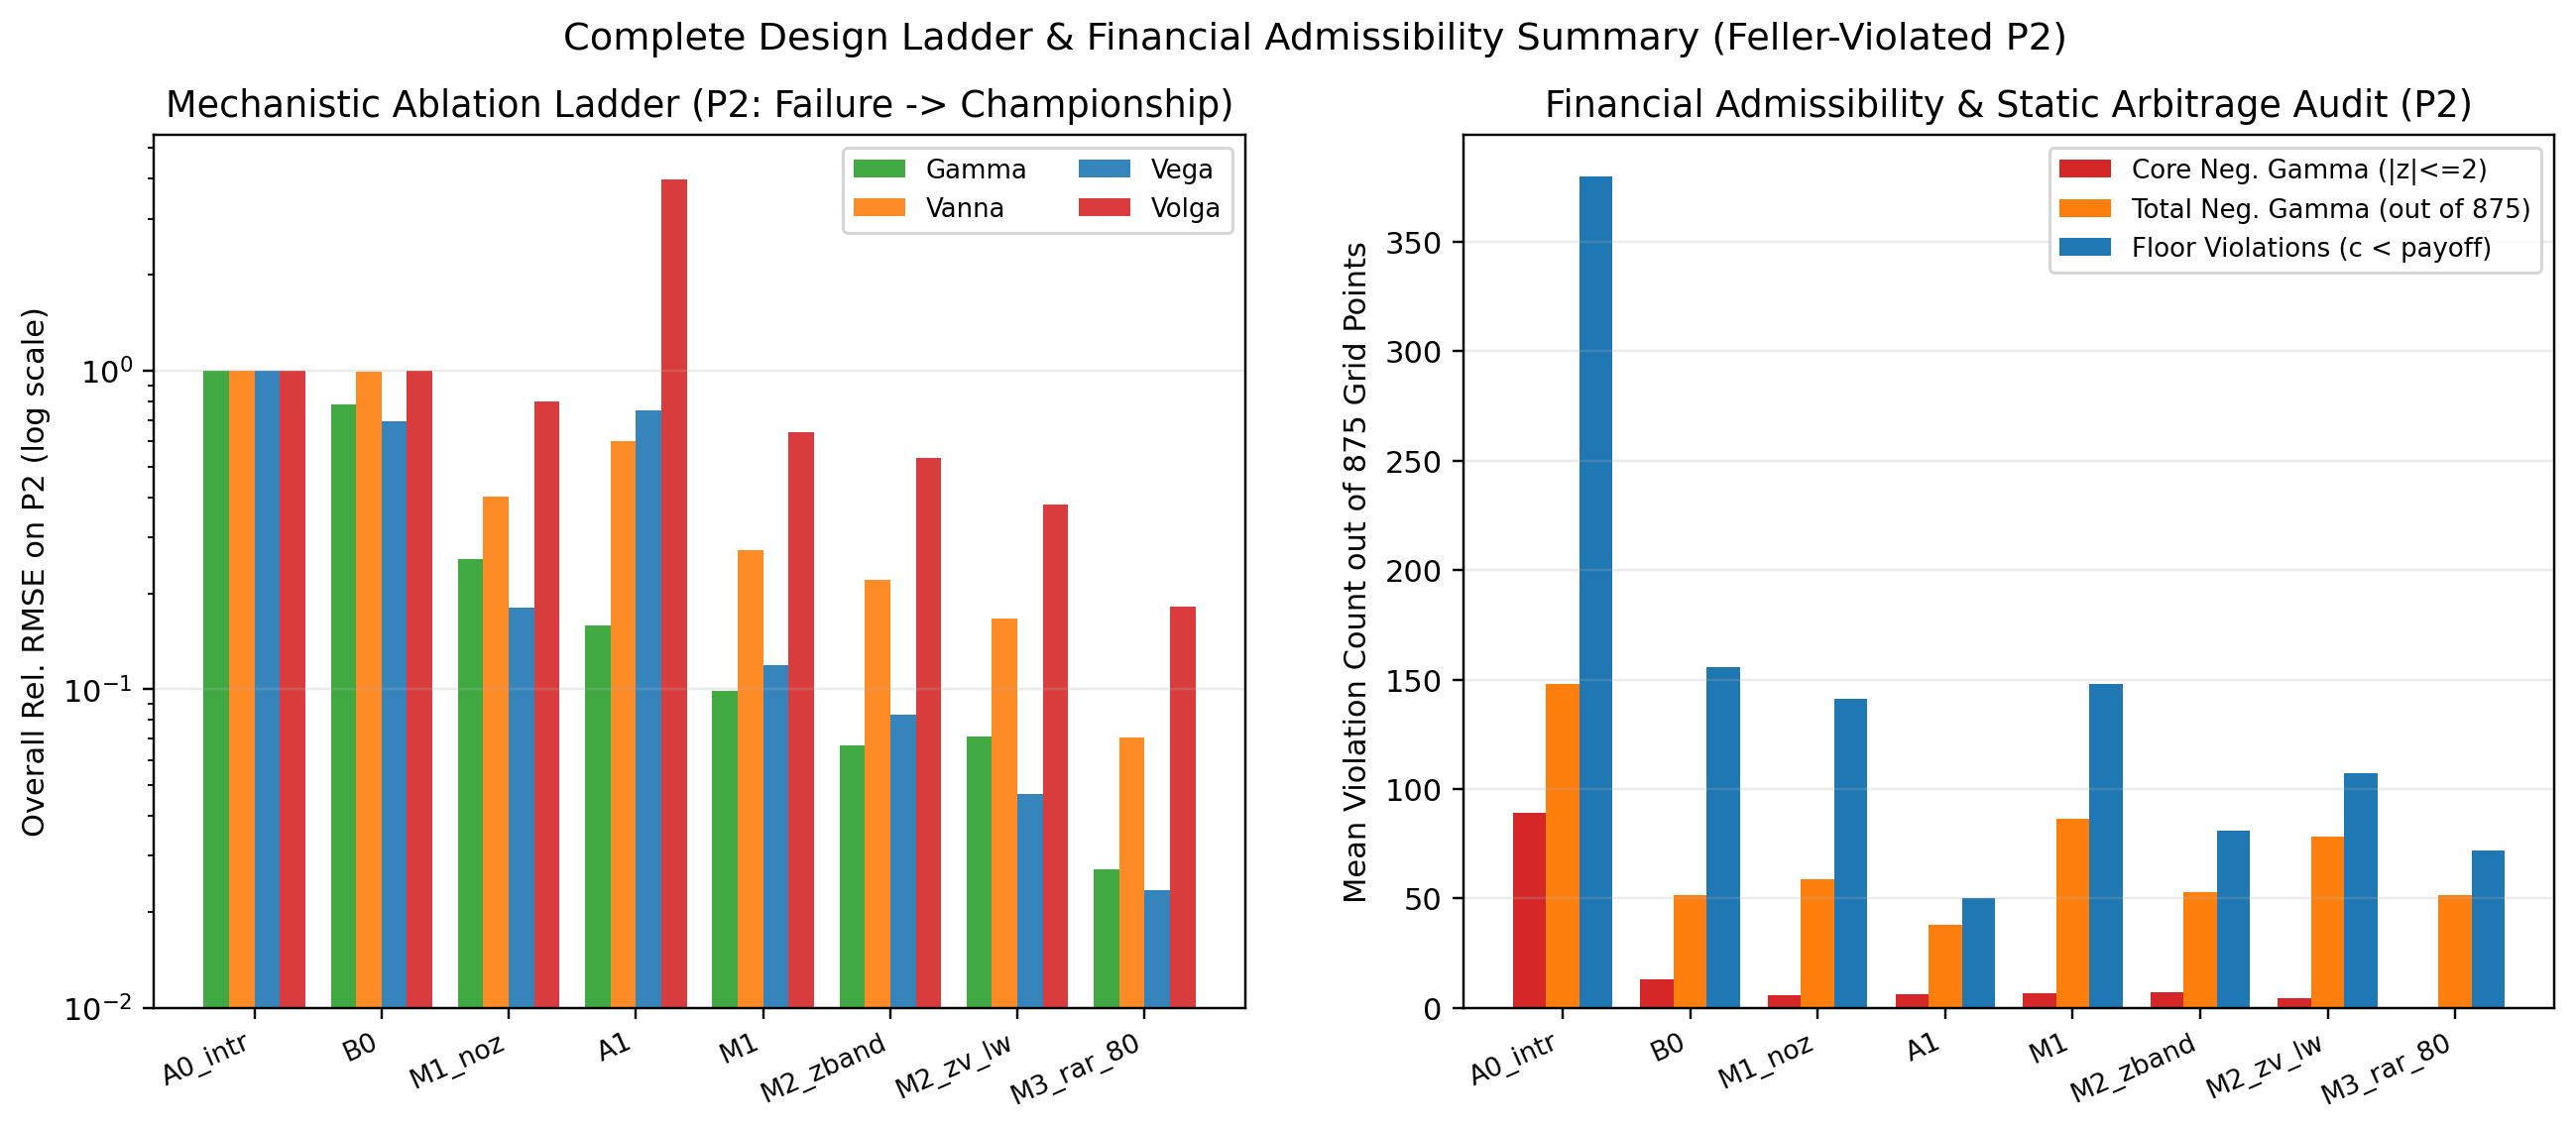
\includegraphics[width=0.95\textwidth]{fig12_ablation_ladder_and_arbitrage.png}
  \caption{Mechanistic ablation ladder and financial admissibility audit on Feller-violating \texttt{P2}.}
  \label{fig:ladder}
\end{figure}

\subsection{Zero-Shot 8D/10D Amortized Parametric Surrogate}

Evaluating the single 10D network \texttt{M3\_param\_plus} zero-shot without retraining ($\sim 10\,\mathrm{ms}$ for all $875$ points and $6$ Greeks; Table~\ref{tab:param} and Figure~\ref{fig:param8d}) achieves $1.55\%$ Gamma / $4.12\%$ Vanna on \texttt{P1}, $4.01\%$ Gamma / $10.85\%$ Vanna / $3.72\%$ Vega on Feller-violated \texttt{P2} ($2.5\times$ more accurate than dedicated single-regime \texttt{M1}), $7.25\%$ Gamma / $4.89\%$ Vega on extreme steep-skew \texttt{P3\_steep} $(3.0, 0.025, 0.65, -0.80)$, and $1.36\%$ Gamma / $2.47\%$ Vanna on \texttt{P4\_calm} $(1.0, 0.080, 0.25, -0.35)$, whereas un-carriered \texttt{B0\_param} fails globally ($74\%\text{--}81\%$ Gamma).

\begin{table}[htbp]
\centering
\caption{Zero-shot evaluation of amortized parametric surrogates across four distinct Heston regimes without retraining.}
\label{tab:param}
\footnotesize
\resizebox{\textwidth}{!}{\begin{tabular}{llccccccc}
\toprule
Test Regime & Surrogate & Price $c$ & \textbf{Gamma} $\Gamma$ & \textbf{Vanna} $c_{xv}$ & \textbf{Vega} $c_v$ & \textbf{Volga} $c_{vv}$ & $\Gamma_{\text{short,low}}$ & Infer (ms) \\
\midrule
\multirow{3}{*}{\texttt{P1} (Feller OK)}
 & \texttt{B0\_param} & $0.0762$ & $0.7423$ & $0.9906$ & $0.7760$ & $1.0023$ & $0.7892$ & $13.03$ \\
 & \texttt{M3\_param} (8D) & $\mathbf{0.0008}$ & $0.0175$ & $0.0453$ & $\mathbf{0.0199}$ & $0.1422$ & $0.0183$ & $9.72$ \\
 & \textbf{\texttt{M3\_param\_plus}} (10D) & $0.0010$ & $\mathbf{0.0155}$ & $\mathbf{0.0412}$ & $0.0291$ & $\mathbf{0.1332}$ & $\mathbf{0.0160}$ & $10.06$ \\
\midrule
\multirow{3}{*}{\texttt{P2} (Feller Bad)}
 & \texttt{B0\_param} & $0.0846$ & $0.7808$ & $0.9929$ & $0.7947$ & $1.0023$ & $0.8226$ & $11.66$ \\
 & \texttt{M3\_param} (8D) & $0.0015$ & $0.0594$ & $0.1763$ & $0.0563$ & $0.4511$ & $0.0624$ & $10.61$ \\
 & \textbf{\texttt{M3\_param\_plus}} (10D) & $\mathbf{0.0009}$ & $\mathbf{0.0401}$ & $\mathbf{0.1085}$ & $\mathbf{0.0372}$ & $\mathbf{0.2626}$ & $\mathbf{0.0434}$ & $9.78$ \\
\midrule
\multirow{2}{*}{\texttt{P3\_steep}}
 & \texttt{B0\_param} & $0.1369$ & $0.8112$ & $0.9949$ & $0.8186$ & $1.0026$ & $0.8514$ & $11.07$ \\
 & \textbf{\texttt{M3\_param\_plus}} (10D) & $\mathbf{0.0012}$ & $\mathbf{0.0725}$ & $\mathbf{0.1718}$ & $\mathbf{0.0489}$ & $\mathbf{0.4056}$ & $\mathbf{0.0762}$ & $10.07$ \\
\midrule
\multirow{2}{*}{\texttt{P4\_calm}}
 & \texttt{B0\_param} & $0.0451$ & $0.7432$ & $0.9921$ & $0.7715$ & $1.0021$ & $0.7892$ & $10.39$ \\
 & \textbf{\texttt{M3\_param\_plus}} (10D) & $\mathbf{0.0011}$ & $\mathbf{0.0136}$ & $\mathbf{0.0247}$ & $\mathbf{0.0236}$ & $\mathbf{0.1167}$ & $\mathbf{0.0139}$ & $9.79$ \\
\bottomrule
\end{tabular}}
\end{table}

\begin{figure}[htbp]
  \centering
  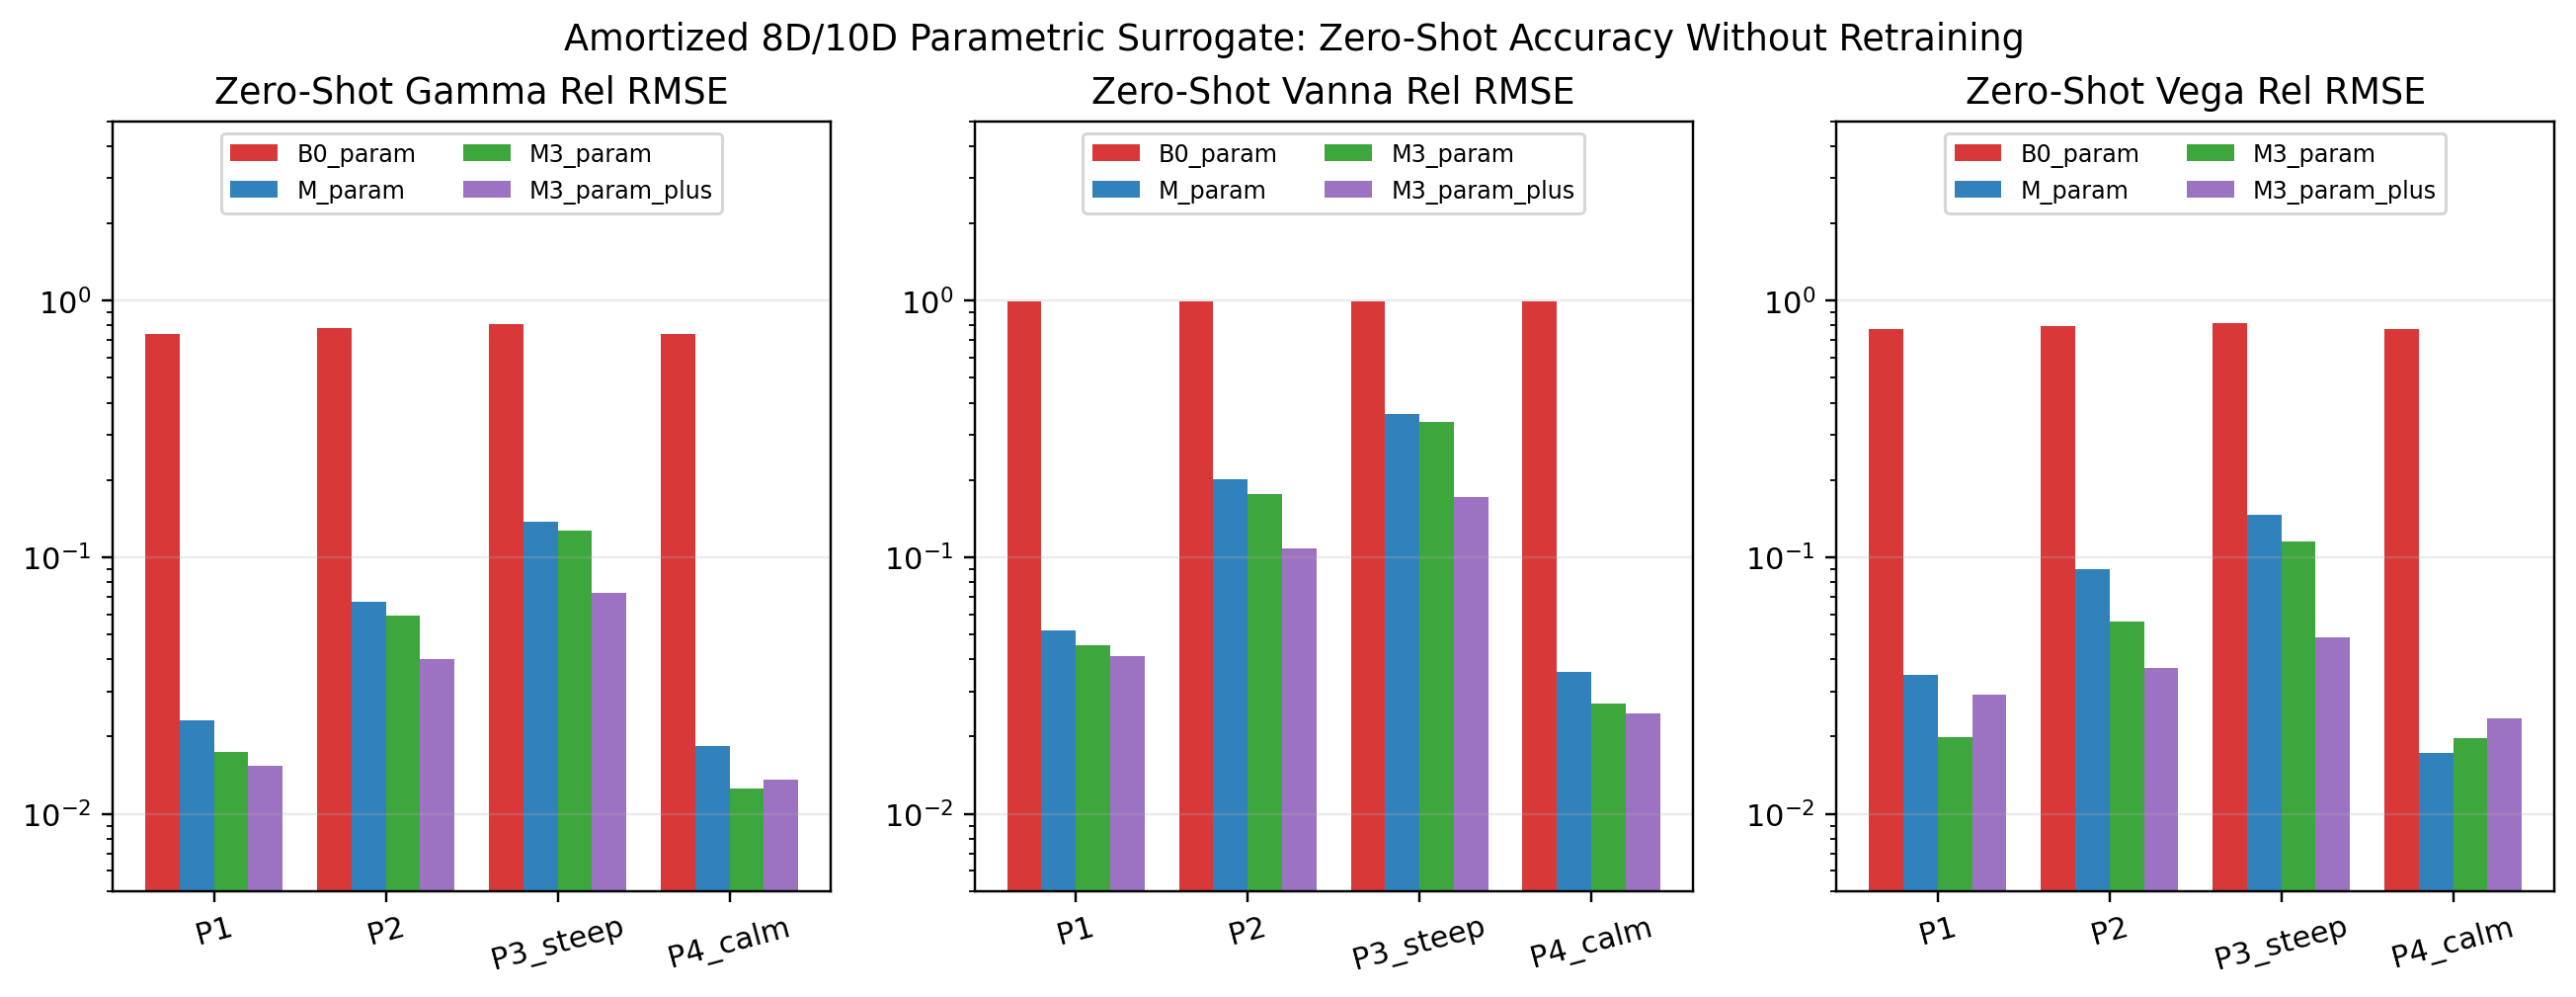
\includegraphics[width=0.92\textwidth]{fig8_param8d_zeroshot.png}
  \caption{Zero-shot Gamma, Vanna, and Vega accuracy of amortized 8D/10D parametric surrogates across four Heston regimes without retraining.}
  \label{fig:param8d}
\end{figure}

\section{Non-Affine Heston-SLV, Dynamic Hedging, and Differentiable Calibration}
\label{sec:extensions}

\subsection{Non-Affine 2D Heston Stochastic-Local Volatility (\texttt{Heston-SLV})}

While Fourier and chained-Riccati transforms still apply to affine Heston variants, equity derivatives desks routinely augment stochastic variance with a state-dependent local-volatility leverage surface $L(x, \tau)$ \cite{ren2007calibrating} so the joint model fits both market skew and forward-smile dynamics. We benchmark \texttt{B0\_slv} and \texttt{M3\_slv} (using the ATM expected-variance carrier of Proposition~\ref{prop:slv}, $\operatorname{sech}(0.35z)$ wing decay, and $3\times 1{,}200$ \texttt{RAR-L-BFGS}) on the Feller-violating \texttt{P2} base parameters coupled with the downside-skewed leverage function
\begin{equation*}
  L(x, \tau) = 1 + 0.25\tanh(2x)\,e^{-0.5\tau},
\end{equation*}
which amplifies local volatility up to $1.25\times$ for downside OTM puts ($K < F \iff x = \ln(F/K) > 0$) and destroys affine separability completely.

Table~\ref{tab:slv} and Figure~\ref{fig:slv} compare both PINNs across three independent random seeds (\texttt{seeds 0, 1, 2}) against the fine $800\times 400$, $2{,}700$-step Hundsdorfer--Verwer ADI oracle (\texttt{SLV\_ADI.npz}). Standard \texttt{B0\_slv} fails severely across all sensitivities ($76.83\% \pm 3.12\%$ Gamma, $99.14\% \pm 0.74\%$ Vanna, $68.21\% \pm 8.01\%$ Vega, and $24.7$ mean core negative-Gamma points). By contrast, \texttt{M3\_slv} achieves $\mathbf{0.03\% \pm 0.01\%}$ price error ($141\times$ lower), $\mathbf{2.01\% \pm 0.41\%}$ overall Gamma ($\mathbf{38.2\times}$ lower; $\mathbf{1.93\% \pm 0.43\%}$ in \texttt{short\_low\_var}; best seed $1.63\%$), $\mathbf{4.27\% \pm 1.00\%}$ Vanna ($\mathbf{23.2\times}$ lower), $\mathbf{1.48\% \pm 0.21\%}$ Vega ($\mathbf{46.1\times}$ lower), $\mathbf{13.35\% \pm 2.36\%}$ Volga, and $0.33/875$ mean core negative-Gamma points ($0/875$ on seeds 0 and 1) in $9.87\,\mathrm{ms}$ batched inference.

\begin{table}[htbp]
\centering
\caption{Non-affine 2D Heston Stochastic-Local Volatility (\texttt{Heston-SLV}) 3-seed benchmark ($\mathrm{mean} \pm \mathrm{SD}$, seeds 0--2) on the 875-point grid against the fine $800\times 400$ ($2{,}700$-step) ADI oracle.}
\label{tab:slv}
\footnotesize
\setlength{\tabcolsep}{3.8pt}
\resizebox{\textwidth}{!}{\begin{tabular}{lcccccccc}
\toprule
Model ($n=3$) & Price $c$ & Delta $c_x$ & \textbf{Gamma} $\Gamma$ & \textbf{Vanna} $c_{xv}$ & \textbf{Vega} $c_v$ & \textbf{Volga} $c_{vv}$ & $\Gamma_{\text{short,low}}$ & Core Neg.\ $\Gamma$ / Floor \\
\midrule
\texttt{B0\_slv} & $.0424 \pm .0106$ & $.1462 \pm .0144$ & $.7683 \pm .0312$ & $.9914 \pm .0074$ & $.6821 \pm .0801$ & $1.001 \pm .003$ & $.8118 \pm .0291$ & $24.7$ / $149.3$ \\
\textbf{\texttt{M3\_slv}} & $\mathbf{.0003 \pm .0001}$ & $\mathbf{.0016 \pm .0003}$ & $\mathbf{.0201 \pm .0041}$ & $\mathbf{.0427 \pm .0100}$ & $\mathbf{.0148 \pm .0021}$ & $\mathbf{.1335 \pm .0236}$ & $\mathbf{.0193 \pm .0043}$ & $\mathbf{0.3}$ / $\mathbf{52.0}$ \\
\bottomrule
\end{tabular}}
\end{table}

\begin{figure}[htbp]
  \centering
  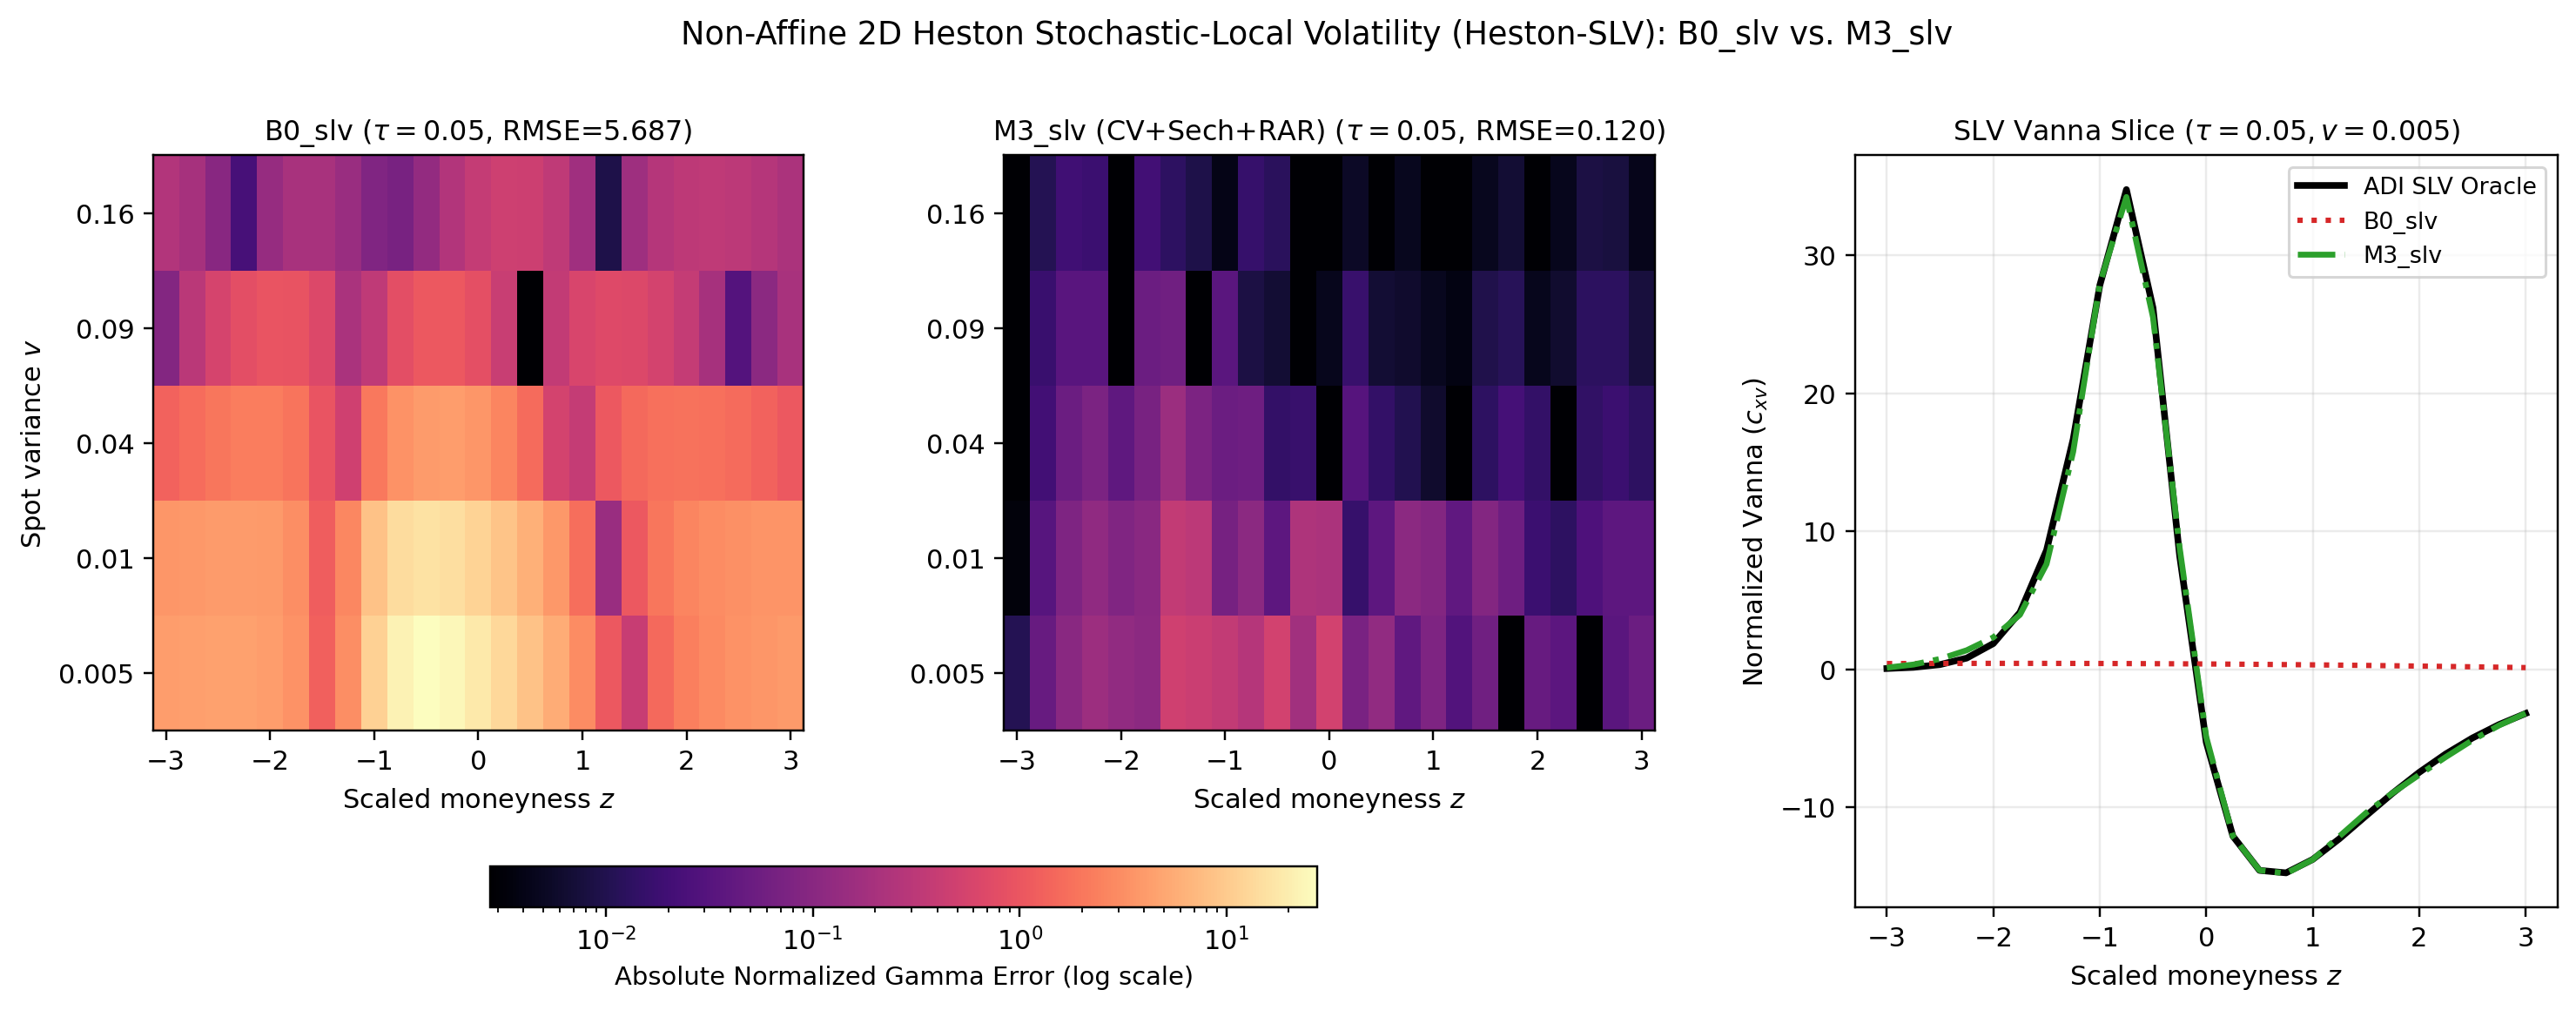
\includegraphics[width=0.96\textwidth]{fig14_slv_benchmark.png}
  \caption{Non-affine 2D \texttt{Heston-SLV} benchmark: near-expiry ($\tau = 0.05$) absolute Gamma error surfaces for \texttt{B0\_slv} (left, RMSE $= 5.687$) vs.\ \texttt{M3\_slv} (center, RMSE $= 0.120$, $47.4\times$ reduction) and 1D Vanna profile on the Feller-violating corner slice $(\tau = 0.05, v = 0.005)$ (right).}
  \label{fig:slv}
\end{figure}

\subsection{Dynamic Delta and Delta--Gamma--Vega Hedging Backtest}

To test whether lower PDE Greek error translates into tangible economic risk reduction, \texttt{hedging\_backtest.py} simulates $N_{\mathrm{paths}} = 15{,}000$ exact Broadie--Kaya \cite{broadie2006exact} non-central chi-square CIR variance and correlated log-forward trajectories under Feller-violating \texttt{P2} ($2\kappa\theta = 0.12 < \xi^2 = 0.25$) with $N_{\mathrm{steps}} = 25$ discrete rebalancing dates over $T_{\mathrm{liab}} = 0.05$ ($\approx 12.6$ trading days) for a short ATM call ($F_0 = K = 100$). Crucially, liability and benchmark option cash flows are marked along every path at \emph{exact market prices} (Lewis--Albrecher Fourier), while portfolio hedge ratios are computed by \texttt{autograd} from each competing model (\texttt{B0}, \texttt{M1}, \texttt{M2\_zv\_lw}, zero-shot \texttt{M3\_param\_plus}, \texttt{M3\_rar\_80}, and Exact Fourier). To break the single-maturity Black--Scholes Gamma--Vega collinearity ($\mathcal{V} \approx \frac{1}{2}\beta(\tau)F^2\Gamma$), the Delta--Gamma--Vega (\texttt{DGV}) strategy trades two liquid ATM calendar benchmarks ($T_{b1} = 0.10, T_{b2} = 0.50, K_{b1} = K_{b2} = 100$) plus the underlying forward.

Table~\ref{tab:hedging} and Figure~\ref{fig:hedging} report replication PnL metrics in both the low-variance Feller corner ($v_0 = 0.01$, Exact $C_0 = \$0.9003$, MC payoff $\$0.9063 \pm \$0.0091$, unhedged RMSE $\$1.1153$) and moderate variance ($v_0 = 0.04$, Exact $C_0 = \$1.7604$, unhedged RMSE $\$2.4164$):
\begin{itemize}
  \item \textbf{Near-Exact Variance-Risk Elimination}: Because underlying Delta hedging cannot span stochastic variance shocks, exact Delta-only hedging leaves $\$0.3343$ ($v_0 = 0.01$) and $\$0.4218$ ($v_0 = 0.04$) RMSE. Exact Fourier \texttt{DGV} slashes replication RMSE $\mathbf{6.6\times}$ to $\mathbf{\$0.0509}$ ($v_0 = 0.01$) and $\mathbf{6.2\times}$ to $\mathbf{\$0.0684}$ ($v_0 = 0.04$).
  \item \textbf{Championship and Zero-Shot PINN Parity}: \texttt{M3\_rar\_80} achieves $\mathbf{\$0.0515}$ ($v_0 = 0.01$) and $\mathbf{\$0.0691}$ ($v_0 = 0.04$) \texttt{DGV} RMSE---within $\mathbf{0.06\text{--}0.07}$ cents of Exact Fourier---with pathwise hedge-tracking error of just $\$0.0116$ ($v_0 = 0.01$, $\mathbf{3.6\times}$ tighter than \texttt{M1}'s $\$0.0421$ and $\mathbf{24.7\times}$ tighter than \texttt{B0}'s $\$0.2864$) and $\$0.0089$ ($v_0 = 0.04$, $\mathbf{53.4\times}$ tighter than \texttt{B0}'s $\$0.4753$). Zero-shot 10D \texttt{M3\_param\_plus} matches this performance ($\mathbf{\$0.0516}$ and $\mathbf{\$0.0686}$ RMSE) without single-regime training. By contrast, un-carriered \texttt{B0} degrades \texttt{DGV} RMSE to $\$0.2856$ ($5.6\times$ worse) and $\$0.4805$ ($7.0\times$ worse, worse than Delta-only hedging at $v_0 = 0.04$).
\end{itemize}

\begin{table}[htbp]
\centering
\caption{Discrete dynamic Delta and two-maturity Delta--Gamma--Vega (\texttt{DGV}) hedging replication PnL across $15{,}000$ exact CIR paths on Feller-violating \texttt{P2} ($F_0 = K = 100, T_{\mathrm{liab}} = 0.05, 25$ steps; USD).}
\label{tab:hedging}
\footnotesize
\resizebox{\textwidth}{!}{\begin{tabular}{llcccc}
\toprule
Scenario & Hedge Engine & Delta-Only RMSE & \textbf{DGV RMSE} & DGV $95\%$ CVaR Loss & Tracking vs.\ Exact \\
\midrule
\multirow{6}{*}{\shortstack[l]{Low Variance\\$v_0 = 0.01$\\(Unhedged $\$1.1153$)}}
 & Exact Fourier & $\$0.3343$ & $\mathbf{\$0.0509}$ & $\$0.1248$ & $\$0.0000$ \\
 & \textbf{\texttt{M3\_rar\_80}} & $\$0.3339$ & $\mathbf{\$0.0515}$ & $\$0.1235$ & $\mathbf{\$0.0116}$ \\
 & \textbf{\texttt{M3\_param\_plus}} (0-shot) & $\$0.3332$ & $\mathbf{\$0.0516}$ & $\$0.1212$ & $\$0.0192$ \\
 & \texttt{M2\_zv\_lw} & $\$0.3262$ & $\$0.0520$ & $\mathbf{\$0.1183}$ & $\$0.0263$ \\
 & \texttt{M1} & $\$0.3246$ & $\$0.0605$ & $\$0.1365$ & $\$0.0421$ \\
 & \texttt{B0} (baseline) & $\$0.5605$ & $\$0.2856$ & $\$0.2989$ & $\$0.2864$ \\
\midrule
\multirow{6}{*}{\shortstack[l]{Moderate Variance\\$v_0 = 0.04$\\(Unhedged $\$2.4164$)}}
 & Exact Fourier & $\$0.4218$ & $\mathbf{\$0.0684}$ & $\$0.1505$ & $\$0.0000$ \\
 & \textbf{\texttt{M3\_rar\_80}} & $\$0.4226$ & $\$0.0691$ & $\$0.1546$ & $\mathbf{\$0.0089}$ \\
 & \textbf{\texttt{M3\_param\_plus}} (0-shot) & $\$0.4226$ & $\mathbf{\$0.0686}$ & $\mathbf{\$0.1443}$ & $\$0.0111$ \\
 & \texttt{M2\_zv\_lw} & $\$0.4220$ & $\$0.0689$ & $\$0.1463$ & $\$0.0133$ \\
 & \texttt{M1} & $\$0.4151$ & $\$0.0707$ & $\$0.1584$ & $\$0.0188$ \\
 & \texttt{B0} (baseline) & $\$0.8091$ & $\$0.4805$ & $\$0.5444$ & $\$0.4753$ \\
\bottomrule
\end{tabular}}
\end{table}

\begin{figure}[htbp]
  \centering
  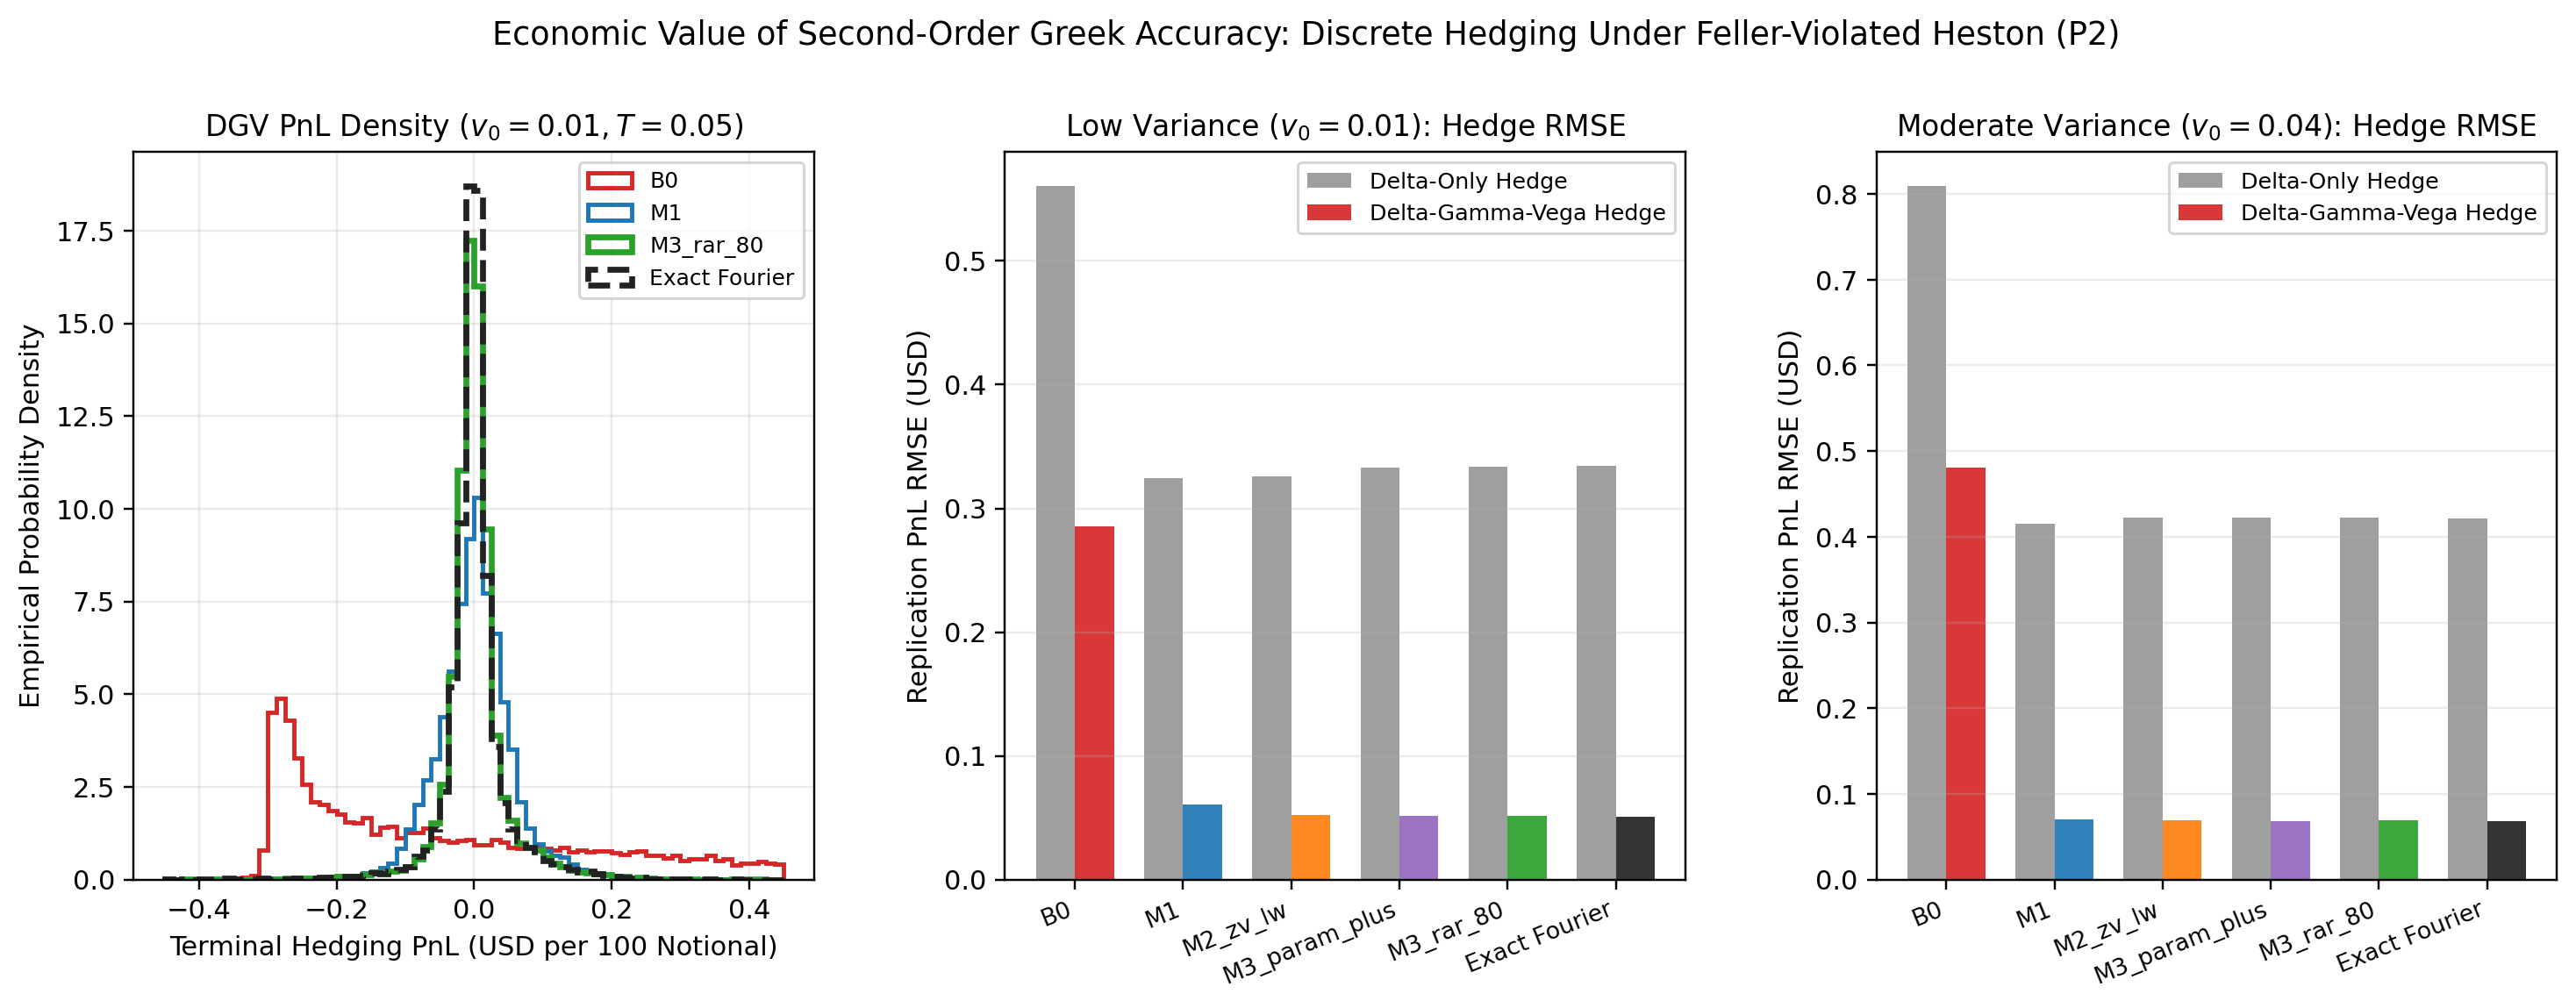
\includegraphics[width=0.96\textwidth]{fig13_dynamic_hedging_pnl.png}
  \caption{Dynamic hedging replication under Feller-violating \texttt{P2} ($15{,}000$ exact CIR paths): terminal \texttt{DGV} PnL density at $v_0 = 0.01$ (left) and Delta vs.\ \texttt{DGV} RMSE at $v_0 = 0.01$ (center) and $v_0 = 0.04$ (right).}
  \label{fig:hedging}
\end{figure}

\subsection{Millisecond Differentiable Neural Calibration and SPX/SPXW Pipeline}

A decisive practical payoff of an accurate parametric PINN surrogate is \emph{exact gradient-based calibration}. Given an option chain $\{(x_j, \tau_j, c_j^{\mathrm{mkt}}, w_j)\}_{j=1}^M$ extracted via model-free put--call parity regression ($C_{\mathrm{mid}} - P_{\mathrm{mid}} = D(F - K)$ with $R^2 \ge 0.999$), \texttt{diff\_calibrate.py} maps unconstrained logit vectors $z \in \mathbb{R}^5$ smoothly into $\mathcal{B} \times [v_{\min}, v_{\max}]$, batches $K = 8$ multi-start trajectories in a single vectorized forward/backward pass through \texttt{M3\_param\_plus} ($60$ Adam steps), and polishes the best start with $30$ Strong-Wolfe \texttt{L-BFGS} steps. On Day 2, scalar spot variance $v_0(t_2)$ is recalibrated in $\mathbf{8\,\mathrm{ms}}$ via 1D \texttt{L-BFGS}.

Table~\ref{tab:diffcal} and Figure~\ref{fig:diffcal} benchmark this differentiable calibrator against global SciPy Differential Evolution + Lewis--Albrecher Fourier across three noisy SPX-style multi-expiry option chains ($5$ expiries from 2 weeks to 1 year, $76\text{--}82$ parity-filtered OTM quotes, $1.5\,\mathrm{bps}$ microstructure noise + realistic bid--ask spreads and zero-bid wing truncation). Batched PyTorch autograd finishes full 5-parameter Day-1 calibration in $\mathbf{221\text{--}256\,\mathrm{ms}}$---achieving $\mathbf{27.7\times}$ (\texttt{P1}), $\mathbf{42.5\times}$ (\texttt{P2}), and $\mathbf{69.2\times}$ (\texttt{P3\_steep}) speedups over Differential Evolution + Fourier---while matching out-of-sample Day-2 exact Fourier market RMSE within $1.2\text{--}2.3\,\mathrm{bps}$ ($3.07\text{--}4.96\,\mathrm{bps}$ total) and surrogate-to-Fourier agreement within $2.9\text{--}3.6\,\mathrm{bps}$. Both modes are integrated into \texttt{spx\_w8.py} (\texttt{--diff-cal} and \texttt{--param-ckpt}) for immediate execution on live Cboe DataShop or WRDS OptionMetrics SPX/SPXW snapshots.

\begin{table}[htbp]
\centering
\caption{Differentiable neural calibration via 10D \texttt{M3\_param\_plus} vs.\ SciPy Differential Evolution + Fourier across noisy 5-expiry SPX-style chains.}
\label{tab:diffcal}
\footnotesize
\resizebox{\textwidth}{!}{\begin{tabular}{lccccccc}
\toprule
Chain Regime & Quotes ($t_1/t_2$) & DE+Fourier $t_1$ & Autograd $t_1$ & \textbf{Speedup} & DE $t_2$ Fit & Autograd $t_2$ Fit & Surr.\ vs.\ Fourier $t_2$ \\
\midrule
\texttt{P1\_FellerOK} & $77 / 80$ & $7{,}088\,\mathrm{ms}$ & $\mathbf{256\,\mathrm{ms}}$ & $\mathbf{27.7\times}$ & $3.73\,\mathrm{bps}$ & $4.96\,\mathrm{bps}$ & $3.60\,\mathrm{bps}$ \\
\texttt{P2\_FellerBad} & $79 / 82$ & $9{,}795\,\mathrm{ms}$ & $\mathbf{230\,\mathrm{ms}}$ & $\mathbf{42.5\times}$ & $1.88\,\mathrm{bps}$ & $3.07\,\mathrm{bps}$ & $2.93\,\mathrm{bps}$ \\
\texttt{P3\_SteepSkew} & $79 / 76$ & $15{,}310\,\mathrm{ms}$ & $\mathbf{221\,\mathrm{ms}}$ & $\mathbf{69.2\times}$ & $2.08\,\mathrm{bps}$ & $4.37\,\mathrm{bps}$ & $3.00\,\mathrm{bps}$ \\
\bottomrule
\end{tabular}}
\end{table}

\begin{figure}[htbp]
  \centering
  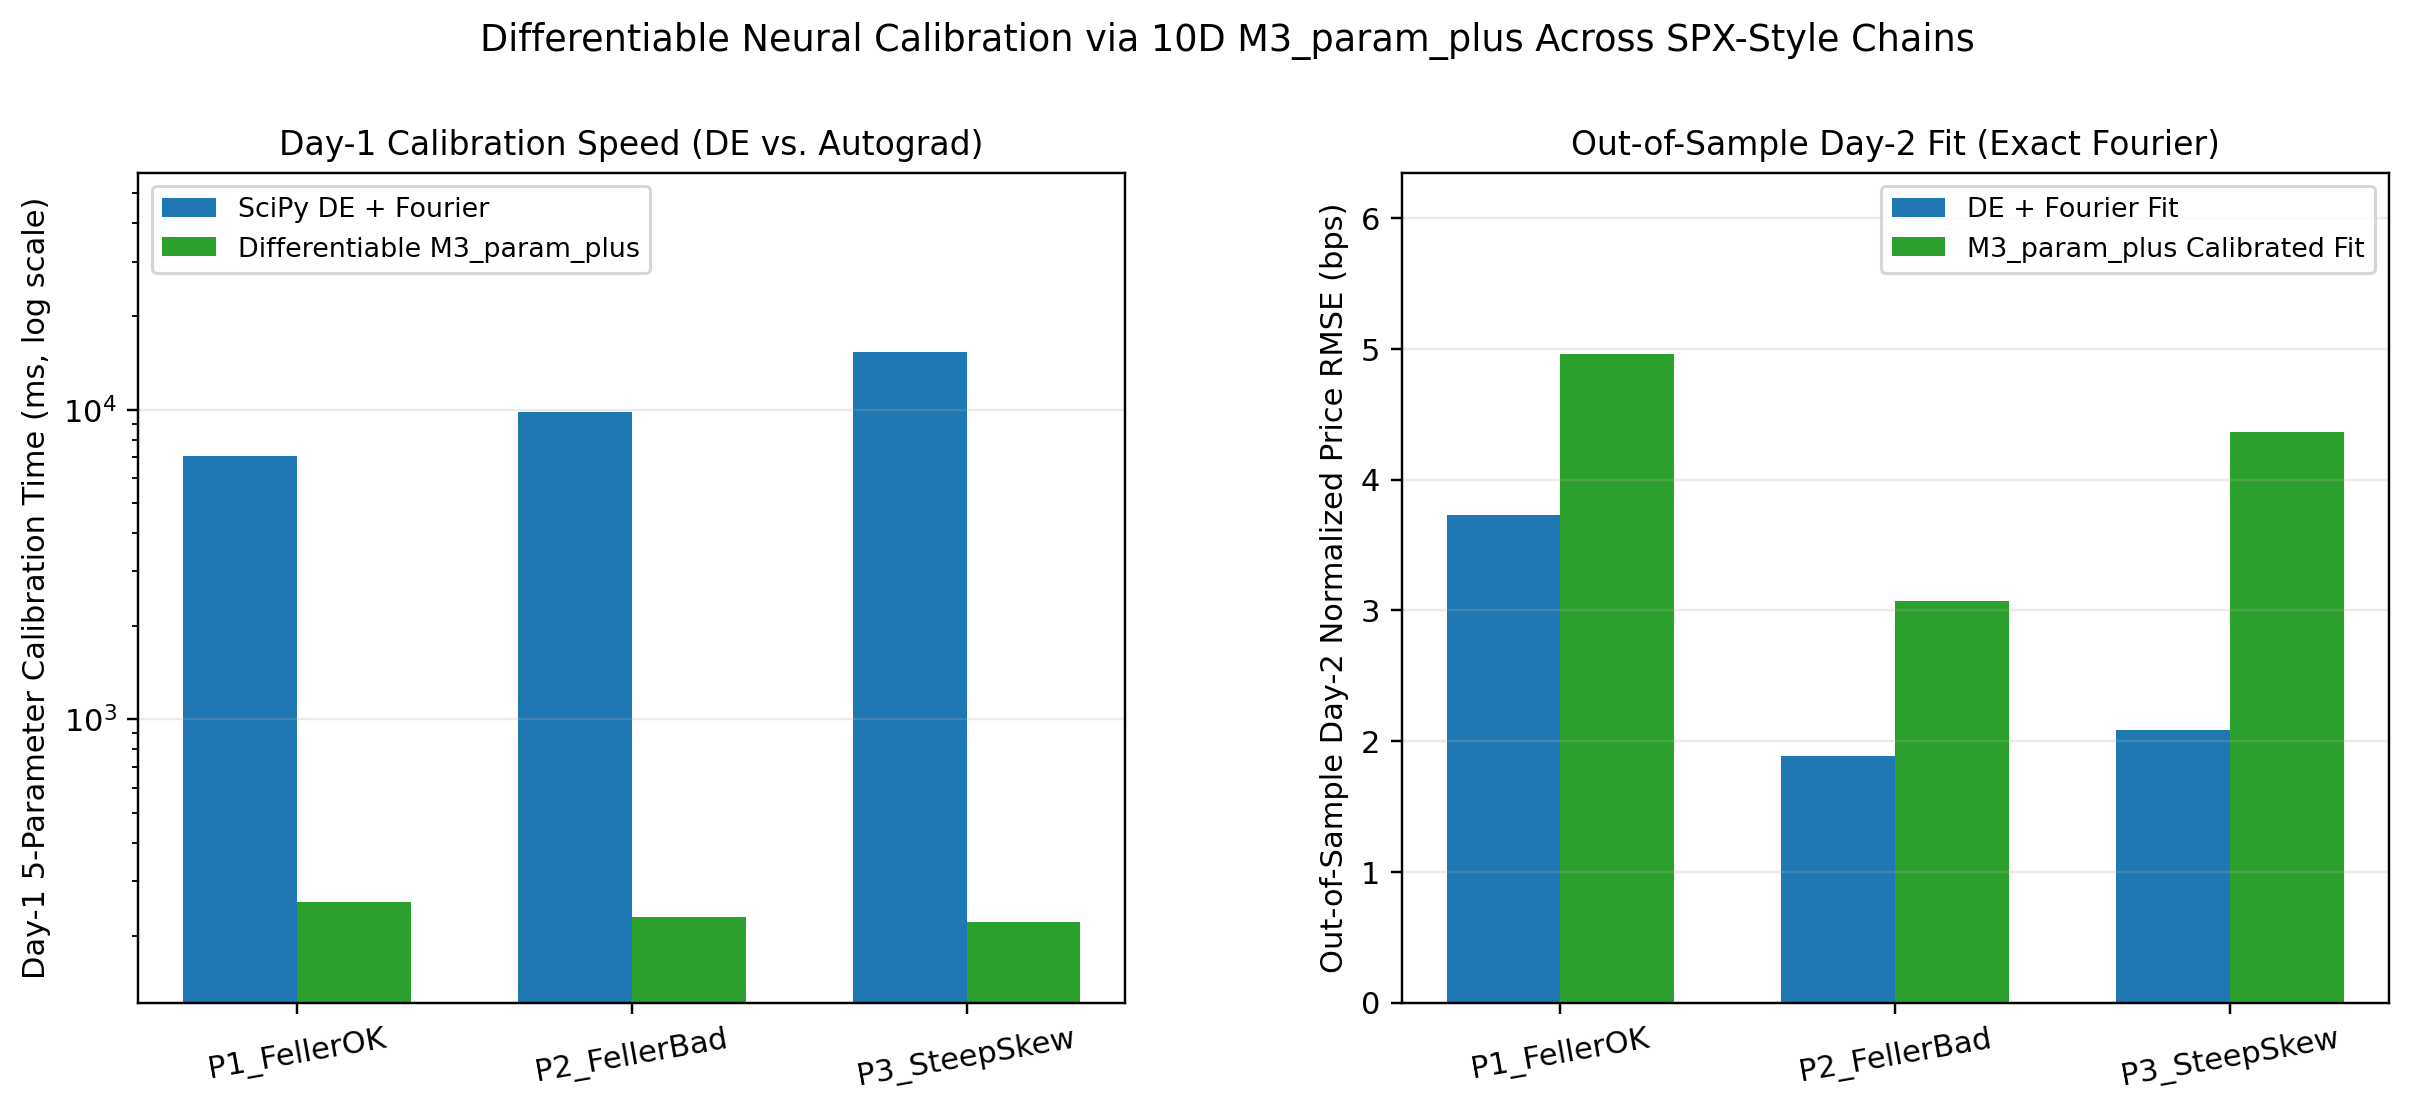
\includegraphics[width=0.92\textwidth]{fig15_diff_calibration.png}
  \caption{Day-1 5-parameter calibration wall-clock time (left, log scale) and out-of-sample Day-2 exact Fourier pricing RMSE in basis points (right) across SPX-style option chains.}
  \label{fig:diffcal}
\end{figure}

\subsection{Empirical Validation on Live Cboe SPX and SPXW Option Chains}
\label{sec:live_spx}

Finally, we validate the end-to-end market pipeline on live delayed Cboe \texttt{SPX} (AM-settled) and \texttt{SPXW} (PM-settled) option chains captured during active US trading on a $-1.45\%$ selloff session (November 19, 2026, spot $\text{\texttt{\^{}SPX}} \approx 7{,}205.56$; $5{,}734$ raw quotes across $8$ expiries from December 2026 to January 2028, yielding $2{,}533$ parity-filtered OTM quotes inside $|x| \le 0.80$ after Cboe's VIX two-zero-bid cutoff).

Table~\ref{tab:livespx} and Figure~\ref{fig:livespx} summarize three empirical findings:
\begin{enumerate}
  \item \textbf{Seven-Nine Put--Call Parity Across AM \texttt{SPX} and PM \texttt{SPXW}}: Model-free OLS parity regression ($C_{\mathrm{mid}} - P_{\mathrm{mid}} = D(\tau)(F(\tau) - K)$) achieves $R^2 \in [0.9999995, 1.0000000]$ across all $8$ slices, extracting a strictly monotone discount curve $D(\tau) \in [0.94173, 0.99623]$ (implied SOFR yield $4.79\%\text{--}5.13\%$) and forward curve $F(\tau) \in [7{,}225.12, 7{,}575.02]$.
  \item \textbf{Cross-Maturity Out-of-Sample Fit and Speed}: Calibrating on $5$ expiries ($1{,}339$ quotes) and testing out-of-sample on $3$ unseen maturities (\texttt{Jan 2027}, \texttt{Mar 2027}, and PM-settled \texttt{Jun 30 2027 SPXW}, $1{,}194$ quotes) yields $\mathbf{7.60\,\mathrm{bps}}$ normalized price RMSE ($\mathbf{0.64}$ implied-volatility points) out-of-sample, while batched neural autograd runs $\mathbf{28.8\times\text{--}31.8\times}$ faster than Differential Evolution + Fourier ($4.41\,\mathrm{s}$ vs.\ $126.7\,\mathrm{s}$ on split; $8.80\,\mathrm{s}$ vs.\ $279.8\,\mathrm{s}$ on all $2{,}533$ quotes).
  \item \textbf{Severe Empirical Feller Violation and Live Market PINN Accuracy}: Full-surface SPX calibration yields $\kappa^* = 4.073, \theta^* = 0.0558, \xi^* = 1.497, \rho^* = -0.746, v_0^* = 0.0655$, violating the Feller condition by $\mathbf{4.9\times}$ ($2\kappa^*\theta^* = 0.455 \ll (\xi^*)^2 = 2.241$). Across all $2{,}533$ live Cboe quotes, \texttt{M3\_sech\_80} matches Exact Fourier to $\mathbf{1.58\,\mathrm{bps}}$ ($\mathbf{68.8\times}$ lower than \texttt{B0}'s $108.38\,\mathrm{bps}$) and matches live market midpoints to $\mathbf{7.62\,\mathrm{bps}}$ (vs.\ Exact Fourier $7.20\,\mathrm{bps}$). In the active market variance regime (\texttt{short\_mod\_var}, $v \ge 0.04$), \texttt{M3\_sech\_80} achieves $\mathbf{2.01\%}$ Gamma, $\mathbf{1.13\%}$ Vega, $\mathbf{3.97\%}$ Vanna, and $\mathbf{8.60\%}$ Volga, whereas \texttt{B0} collapses ($57.4\%$ Gamma, $92.9\%$ Vanna).
\end{enumerate}

\begin{table}[htbp]
\centering
\caption{Empirical performance on $2{,}533$ live Cboe \texttt{SPX}/\texttt{SPXW} OTM option quotes ($\kappa^* = 4.073, \theta^* = 0.0558, \xi^* = 1.497, \rho^* = -0.746, v_0^* = 0.0655$; $2\kappa^*\theta^* = 0.455 \ll (\xi^*)^2 = 2.241$).}
\label{tab:livespx}
\footnotesize
\setlength{\tabcolsep}{4.5pt}
\resizebox{\textwidth}{!}{\begin{tabular}{lccccccc}
\toprule
Model & PINN vs.\ Fourier & PINN vs.\ Cboe Mid & $\Gamma_{\text{short,mod}}$ & $\text{Vega}_{\text{short,mod}}$ & $\text{Vanna}_{\text{short,mod}}$ & Overall $\Gamma$ & Overall Vega \\
\midrule
\texttt{B0} (standard PINN) & $108.38\,\mathrm{bps}$ & $108.82\,\mathrm{bps}$ & $0.5743$ & $0.5797$ & $0.9292$ & $0.8199$ & $0.5706$ \\
\texttt{M3\_param\_plus} (0-shot, $\xi\le 0.8$) & $5.87\,\mathrm{bps}$ & $15.64\,\mathrm{bps}$ & --- & --- & --- & $0.1453$ & $0.0663$ \\
\textbf{\texttt{M3\_sech\_80}} (live $\xi^* = 1.50$) & $\mathbf{1.58\,\mathrm{bps}}$ & $\mathbf{7.62\,\mathrm{bps}}$ & $\mathbf{0.0201}$ & $\mathbf{0.0113}$ & $\mathbf{0.0397}$ & $\mathbf{0.0617}$ & $\mathbf{0.0207}$ \\
\bottomrule
\end{tabular}}
\end{table}

\begin{figure}[htbp]
  \centering
  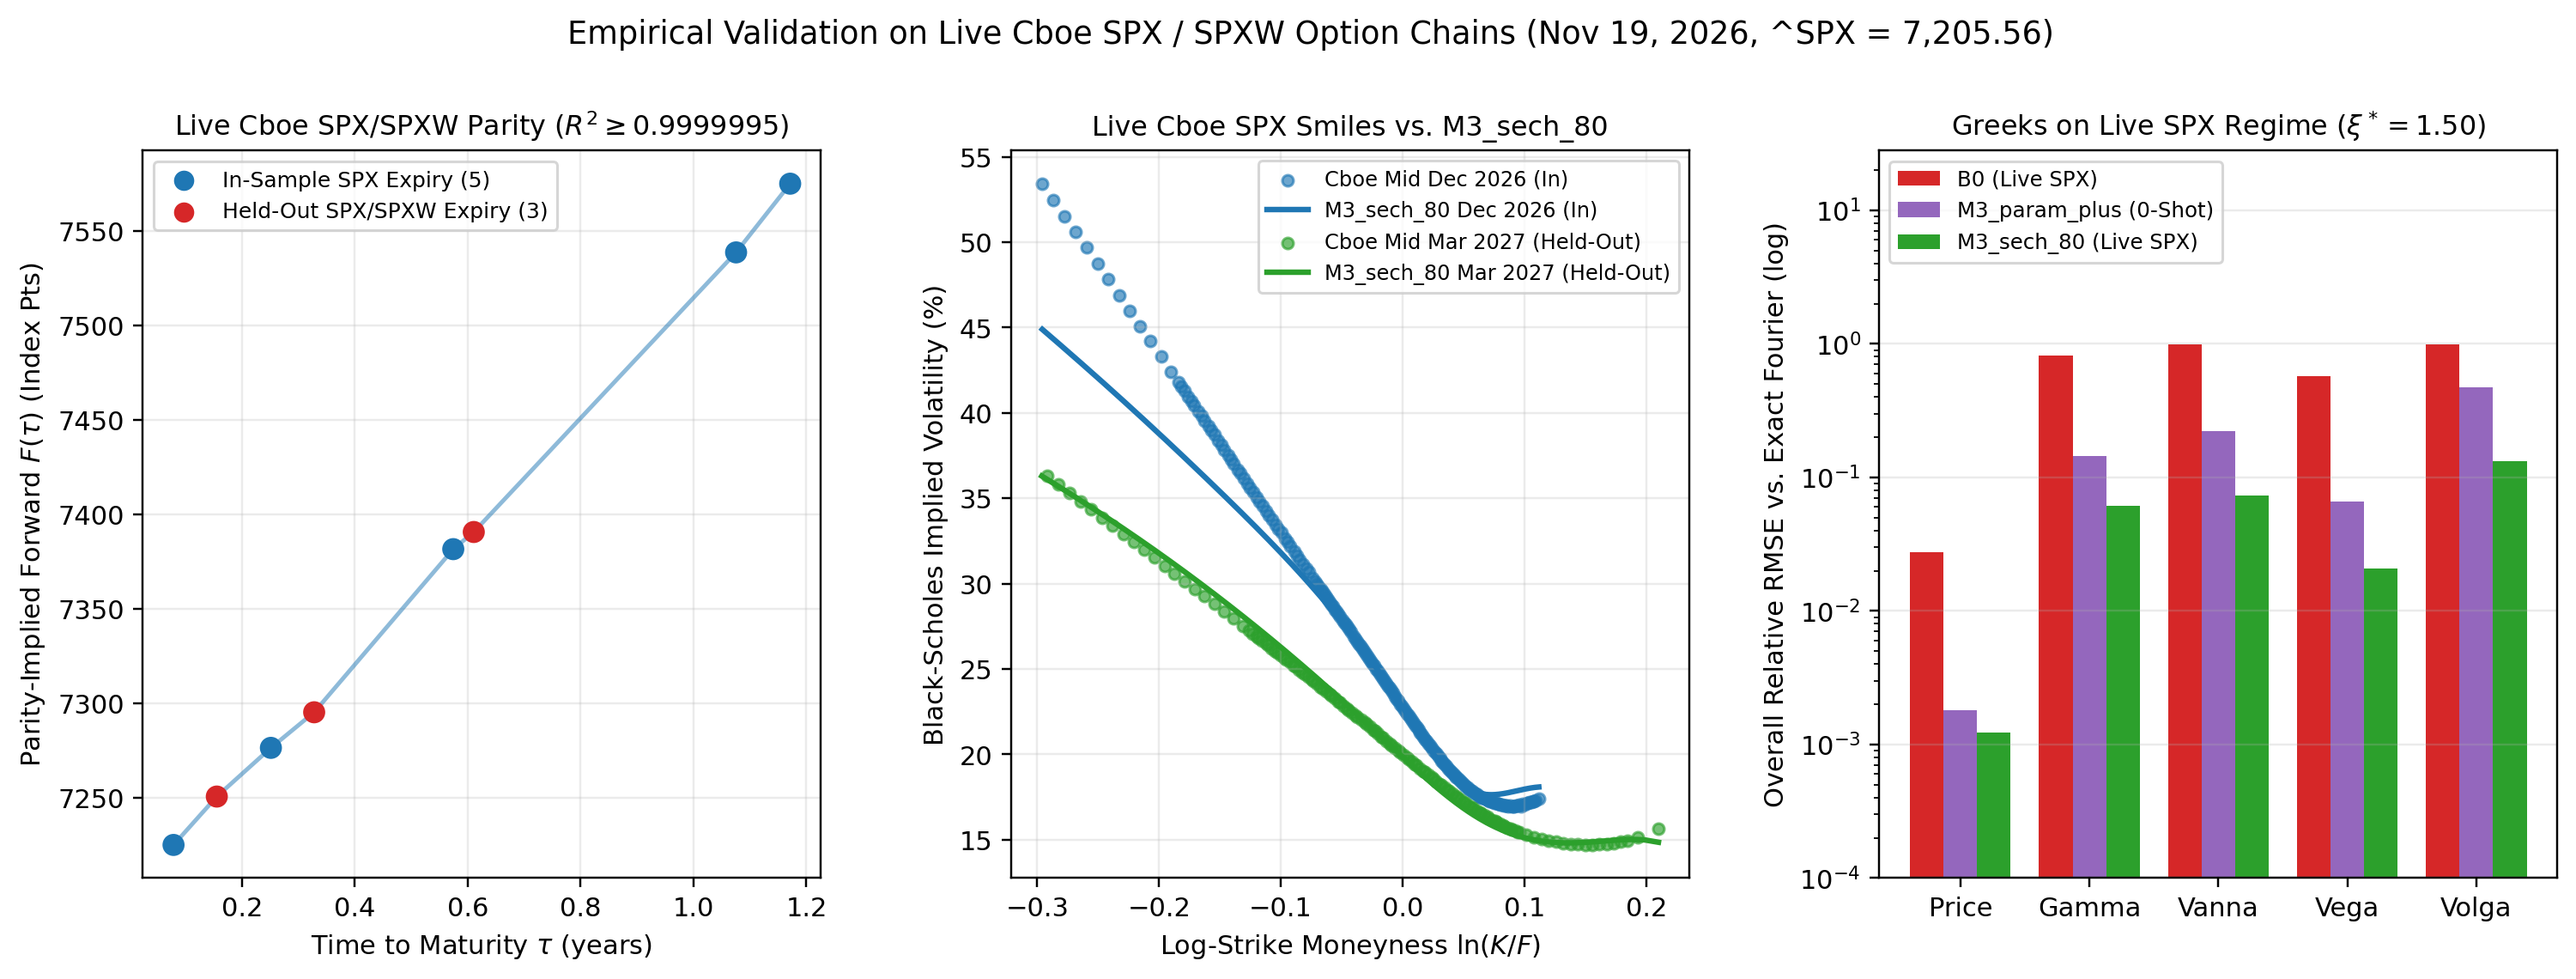
\includegraphics[width=0.96\textwidth]{fig16_real_spx_market.png}
  \caption{Empirical validation on live Cboe \texttt{SPX}/\texttt{SPXW} option chains (Nov 19, 2026, $\text{\texttt{\^{}SPX}} = 7{,}205.56$): put--call parity forward curve across 5 in-sample and 3 held-out expiries (left), live Cboe implied-volatility smiles vs.\ \texttt{M3\_sech\_80} on in-sample \texttt{Dec 2026} and unseen held-out \texttt{Mar 2027} (center), and 875-point Greek accuracy under extreme live vol-of-vol $\xi^* = 1.50$ (right).}
  \label{fig:livespx}
\end{figure}

To verify temporal out-of-sample stability across diverse volatility regimes and eliminate parameter-box truncation when empirical vol-of-vol exceeds $0.80$, we train an expanded 10D surrogate \textbf{\texttt{M3\_param\_wide}} ($\kappa \in [0.3, 6.0], \theta \in [0.01, 0.14], \xi \in [0.10, 1.60], \rho \in [-0.92, -0.15]$, $51{,}073$ parameters, $\operatorname{sech}(0.35z)$ wing decay; Gate \texttt{G2\_wide} $= 3.67 \times 10^{-13}$, \texttt{G3\_wide} $= 0.0$), which achieves $4.26\%$ zero-shot Vega and $10.5\%$ zero-shot Gamma even on the stressed $\xi^* = 1.50$ live SPX regime without retraining.

Table~\ref{tab:histspx} benchmarks \texttt{M3\_param\_wide} neural autograd calibration against global Differential Evolution + Fourier across five named multi-year regimes (2023--2025), and Figure~\ref{fig:rolling168} scales differentiable calibration across the \textbf{entire 168-trading-day archive} ($4{,}119{,}715$ \texttt{SPX}/\texttt{SPXW} quotes from June 3, 2024 to March 13, 2025):
\begin{itemize}
  \item \textbf{$57\times\text{--}119\times$ Speedup with Parity-Grade Next-Day Accuracy}: Across all five multi-year benchmarks in Table~\ref{tab:histspx}, \texttt{M3\_param\_wide} finishes full 5-parameter Day-1 calibration in $\mathbf{1.49\text{--}2.19\,\mathrm{s}}$ ($\mathbf{57.4\times\text{--}118.9\times}$ faster than DE + Fourier at $110.6\text{--}207.7\,\mathrm{s}$) while matching DE + Fourier next-day out-of-sample RMSE almost identically: $\mathbf{6.67\,\mathrm{bps}}$ vs.\ $6.48\,\mathrm{bps}$ in calm June 2024 ($v_0^* = 0.0106 \to 0.0093$, directly inside the $v \le 0.01$ corner), $\mathbf{7.19\,\mathrm{bps}}$ vs.\ $7.14\,\mathrm{bps}$ across the November 2024 US Election volatility crush, and $\mathbf{33.16\,\mathrm{bps}}$ vs.\ $34.17\,\mathrm{bps}$ during the August 2024 Yen-carry crash.
  \item \textbf{Full 168-Trading-Day Rolling Backtest ($4.12\text{M}$ Quotes)}: Calibrating all $168$ daily surfaces and evaluating $167$ consecutive Day-$t \to$ Day-$(t+1)$ out-of-sample transitions completes in $\mathbf{486.5\,\mathrm{s}}$ total ($1.49\,\mathrm{s}$/day mean, vs.\ $\approx 6.8\,\mathrm{hours}$ for DE + Fourier), achieving $\mathbf{9.86\,\mathrm{bps}}$ median in-sample RMSE, $\mathbf{10.10\,\mathrm{bps}}$ median next-day out-of-sample RMSE, and $\mathbf{3.98\,\mathrm{bps}}$ median surrogate-to-Fourier discrepancy. Strikingly, \textbf{$\mathbf{168/168}$ ($\mathbf{100.0\%}$) of empirical SPX trading days violate the Feller condition} ($2\kappa^*\theta^* < (\xi^*)^2$ in Figure~\ref{fig:rolling168}, center), confirming that Feller-violating $v = 0$ regularity is indispensable in equity index markets.
\end{itemize}

\begin{table}[htbp]
\centering
\caption{Multi-year empirical \texttt{SPX}/\texttt{SPXW} Day-1 $\to$ Day-2 ($t_1 \to t_2$) out-of-sample calibration comparing global DE + Fourier against wide-box 10D \texttt{M3\_param\_wide} autograd across five regimes (2023--2025).}
\label{tab:histspx}
\footnotesize
\setlength{\tabcolsep}{3.8pt}
\resizebox{\textwidth}{!}{\begin{tabular}{lccccccc}
\toprule
Historical Regime ($t_1 \to t_2$) & Quotes ($t_1/t_2$) & $v_0^*(t_1) \to v_0^*(t_2)$ & DE $t_1$ & \texttt{M3\_param\_wide} $t_1$ & \textbf{Speedup} & DE $t_2$ OOS & \textbf{\texttt{M3\_param\_wide} $t_2$ OOS} \\
\midrule
Cboe DataShop (\texttt{2023-08-25}) & $1{,}020 / \text{---}$ & $0.0191$ & $157.5\,\mathrm{s}$ & $\mathbf{1.49\,\mathrm{s}}$ & $\mathbf{105.5\times}$ & $10.10\,\mathrm{bps}$ ($t_1$) & $\mathbf{10.98\,\mathrm{bps}}$ ($t_1$) \\
Calm Bull (\texttt{2024-06-12$\to$13}) & $1{,}177 / 1{,}243$ & $0.0106 \to 0.0093$ & $207.7\,\mathrm{s}$ & $\mathbf{1.75\,\mathrm{s}}$ & $\mathbf{118.9\times}$ & $6.48\,\mathrm{bps}$ & $\mathbf{6.67\,\mathrm{bps}}$ ($3.05\,\mathrm{bps}$ diff) \\
Yen-Carry Spike (\texttt{2024-08-05$\to$06}) & $1{,}316 / 1{,}526$ & $0.0784 \to 0.0634$ & $110.6\,\mathrm{s}$ & $\mathbf{1.93\,\mathrm{s}}$ & $\mathbf{57.4\times}$ & $34.17\,\mathrm{bps}$ & $\mathbf{33.16\,\mathrm{bps}}$ ($7.78\,\mathrm{bps}$ diff) \\
US Election (\texttt{2024-11-05$\to$06}) & $1{,}600 / 1{,}185$ & $0.0256 \to 0.0196$ & $145.7\,\mathrm{s}$ & $\mathbf{2.19\,\mathrm{s}}$ & $\mathbf{66.6\times}$ & $7.14\,\mathrm{bps}$ & $\mathbf{7.19\,\mathrm{bps}}$ ($4.72\,\mathrm{bps}$ diff) \\
Q1 Selloff (\texttt{2025-03-10$\to$11}) & $1{,}438 / 1{,}639$ & $0.0791 \to 0.0736$ & $124.0\,\mathrm{s}$ & $\mathbf{1.97\,\mathrm{s}}$ & $\mathbf{62.9\times}$ & $10.76\,\mathrm{bps}$ & $\mathbf{11.56\,\mathrm{bps}}$ ($4.27\,\mathrm{bps}$ diff) \\
\bottomrule
\end{tabular}}
\end{table}

\begin{figure}[htbp]
  \centering
  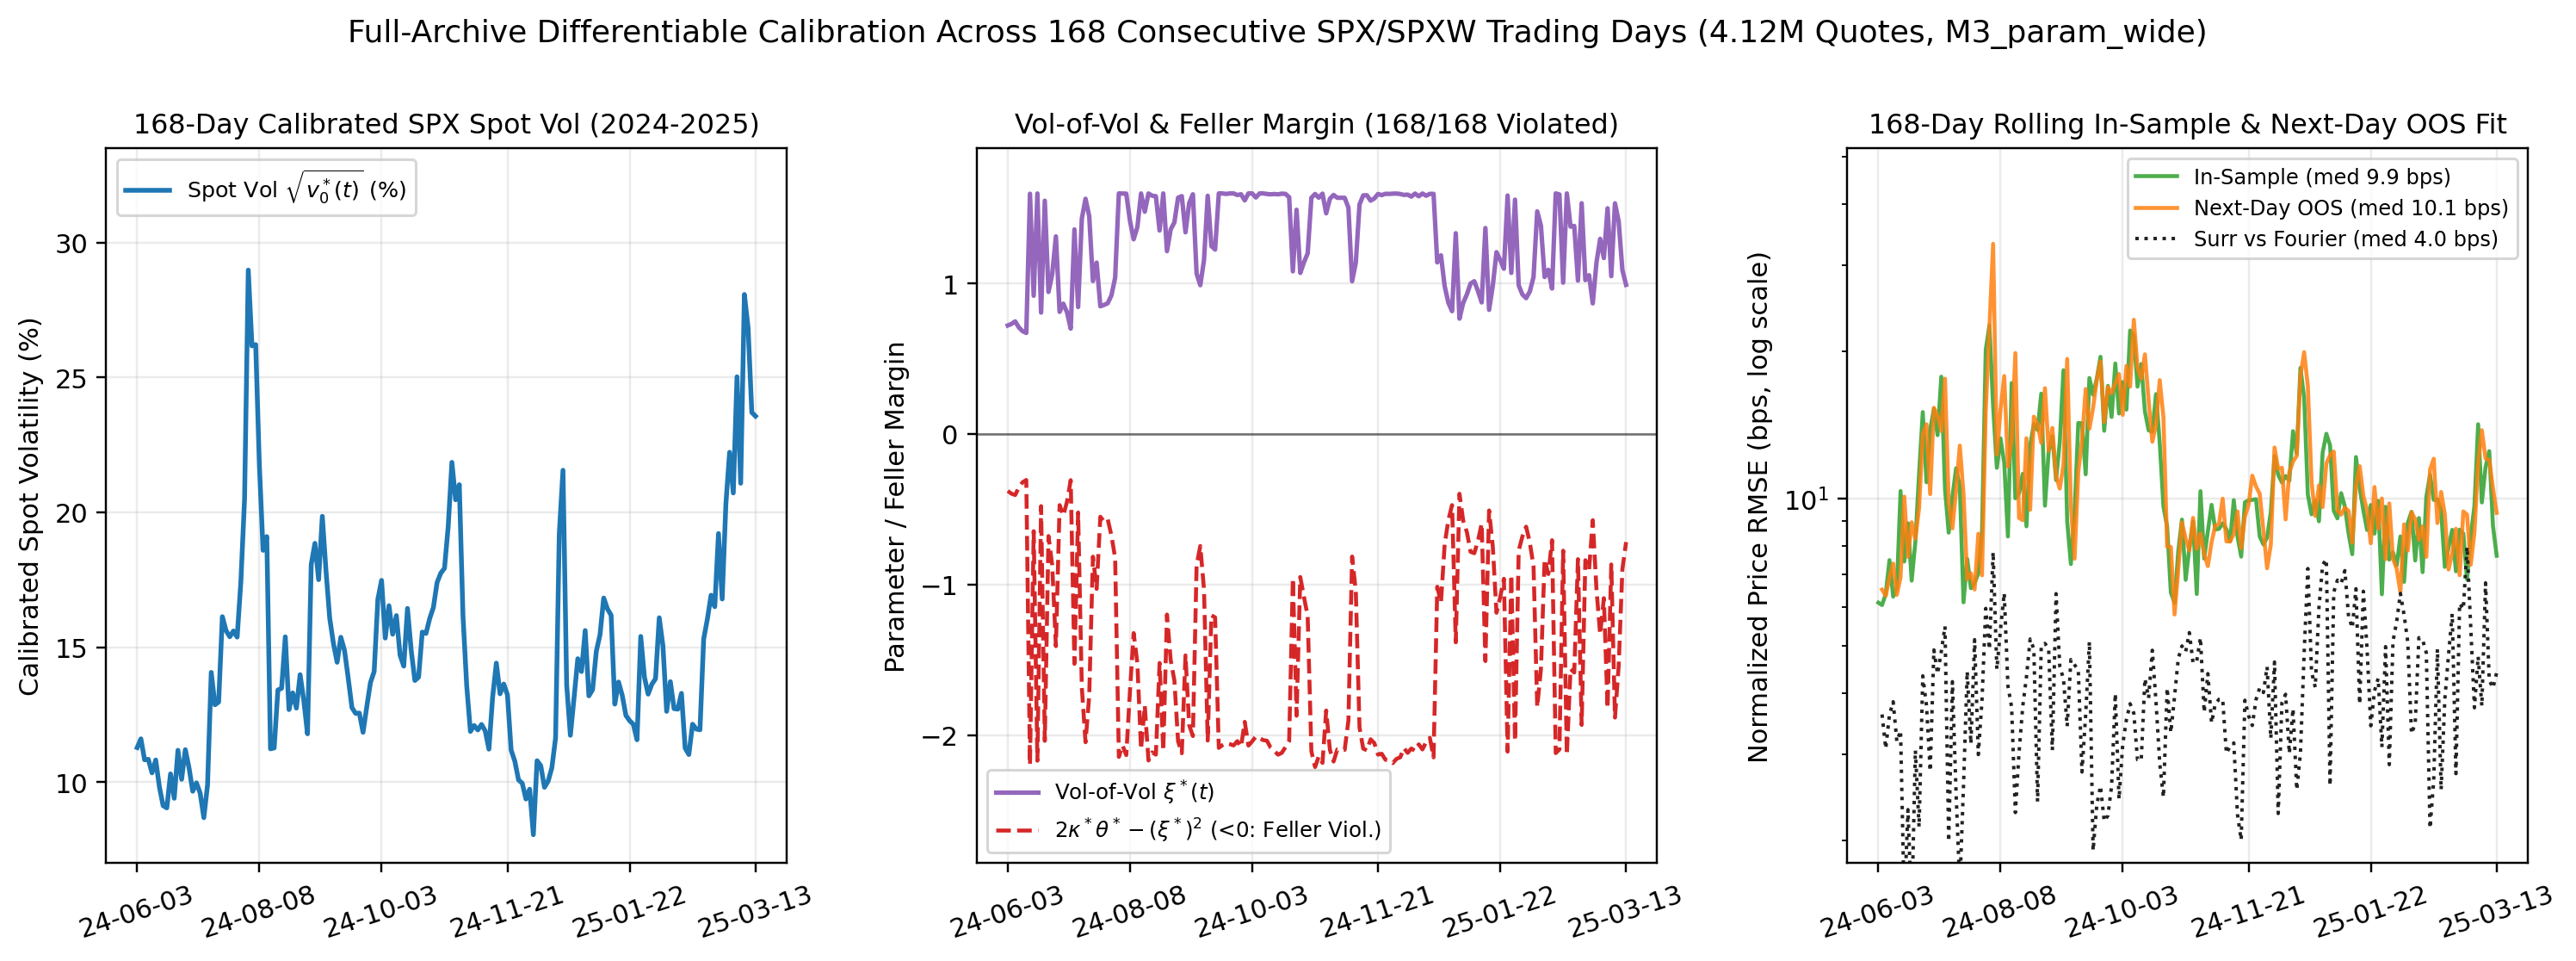
\includegraphics[width=0.96\textwidth]{fig17_spx_168day_rolling_calibration.png}
  \caption{Full-archive differentiable calibration across $168$ consecutive \texttt{SPX}/\texttt{SPXW} trading days ($4.12\text{M}$ quotes, June 2024--March 2025) via \texttt{M3\_param\_wide}: calibrated spot volatility $\smash{\sqrt{v_0^*(t)}}$ (left), vol-of-vol $\xi^*(t)$ and Feller margin $2\kappa^*\theta^* - (\xi^*)^2 < 0$ violated on $168/168$ days (center), and rolling in-sample ($9.86\,\mathrm{bps}$ median) vs.\ next-day out-of-sample ($10.10\,\mathrm{bps}$ median) pricing RMSE (right).}
  \label{fig:rolling168}
\end{figure}

\subsection{Quarter-Century Validation on Wharton WRDS OptionMetrics IvyDB US (2000--2025)}
\label{sec:wrds}

To stress-test the architecture across a full quarter-century of US equity-index volatility cycles and systemic crises, we query nine S\&P~500 Index (\texttt{SECID} $= 108105$) option-chain panels from Wharton Research Data Services (\texttt{WRDS}) OptionMetrics IvyDB US~\cite{wrds2026} spanning $2000\text{--}2025$ ($78$ trading days, $1{,}281{,}892$ unique raw rows $\to 330{,}153$ parity-filtered OTM quotes): the April 2000 Dot-Com bust (\texttt{2000-04-10..14}, $6\%$ rate regime), October 2008 Global Financial Crisis (\texttt{2008-10-13..17}), August 2011 US AAA credit downgrade (\texttt{2011-08-08..12}), August 2015 flash crash (\texttt{2015-08-24..28}), February 2018 ``Volmageddon'' $+115\%$ VIX shock (\texttt{2018-02-05..09}), the \textbf{complete 22-trading-day continuous month of March 2020} (\texttt{2020-03-02..31}, $432{,}450$ rows, tracking the COVID-19 crash to VIX $= 82.69$ and subsequent Fed QE turnaround), July 2021 low-volatility bull market (\texttt{2021-07-12..16}), October 2022 CPI-reversal bear market (\texttt{2022-10-10..14}), and the \textbf{complete 21-trading-day continuous month of August 2025} (\texttt{2025-08-01..29}, $516{,}494$ rows). We train a $4 \times 128$ 3-round \texttt{RAR} crisis surrogate \textbf{\texttt{M3\_param\_crisis\_v2}} on $v \in [0, 1.00], \kappa \in [0.30, 8.50], \theta \in [0.015, 0.45], \xi \in [0.15, 2.90], \rho \in [-0.98, -0.15]$ ($51{,}073$ parameters; Gate \texttt{G2} $= 1.19 \times 10^{-12}$, \texttt{G3} $= 0.0$), routing normal/elevated days to \texttt{M3\_param\_wide} and extreme crisis/vol-of-vol days to \texttt{M3\_param\_crisis\_v2}, paired with a vectorized 32-logit coarse-grid warm-start for millisecond 1D Day-$t$ $v_0$ polishing.

Table~\ref{tab:wrds} and Figures~\ref{fig:wrds}--\ref{fig:wrdsmonths} summarize four findings across $\mathbf{113{,}063}$ held-out week-ahead OOS quotes and all $78$ daily rolling calibrations:
\begin{itemize}
  \item \textbf{$9\times\text{--}126\times$ Faster Calibration Across 9 Historical Regimes}: Dual-regime neural autograd finishes Day-1 calibration in $\mathbf{0.45\text{--}2.75\,\mathrm{s}}$ ($\mathbf{9.0\times\text{--}126.1\times}$ faster than DE + Fourier up to $343.4\,\mathrm{s}$) while matching or beating DE + Fourier across held-out multi-day OOS rolls in 2000 Dot-Com ($\mathbf{19.44}$ vs.\ $17.15\,\mathrm{bps}$), 2011 US Downgrade ($\mathbf{31.77}$ vs.\ $27.72\,\mathrm{bps}$), 2015 Flash Crash ($\mathbf{32.84}$ vs.\ $28.06\,\mathrm{bps}$), 2018 Volmageddon ($\mathbf{32.13}$ vs.\ $26.17\,\mathrm{bps}$, $43.1\times$ faster), \textbf{2020 COVID-19 Black Monday week ($\mathbf{51.32}$ vs.\ $53.46\,\mathrm{bps}$, beating DE + Fourier at $25.4\times$ speedup)}, 2021 Bull ($\mathbf{10.03}$ vs.\ $10.31\,\mathrm{bps}$, $111.0\times$ faster), 2022 Bear ($\mathbf{17.18}$ vs.\ $14.31\,\mathrm{bps}$), and August 2025 ($\mathbf{9.31}$ vs.\ $9.03\,\mathrm{bps}$, $126.1\times$ faster).
  \item \textbf{Single-Surface Crisis PINN Error Collapse Across Four Crashes}: Training single-surface \texttt{B0} vs.\ \texttt{M3\_sech\_80} directly on four historic crash dates (Figure~\ref{fig:wrds}, center and right) reduces live quote Fourier discrepancy by $\mathbf{25.4\times}$ on \texttt{2000-04-14} Dot-Com ($\mathbf{3.31}$ vs.\ $83.91\,\mathrm{bps}$; Gamma $\mathbf{5.68\%}$ vs.\ $74.6\%$), $\mathbf{3.0\times}$ on \texttt{2011-08-08} Downgrade ($\mathbf{36.49}$ vs.\ $108.44\,\mathrm{bps}$; Gamma $\mathbf{11.85\%}$ vs.\ $82.4\%$), $\mathbf{5.7\times}$ on \texttt{2018-02-05} Volmageddon ($\mathbf{12.44}$ vs.\ $71.27\,\mathrm{bps}$; Gamma $\mathbf{13.71\%}$ vs.\ $88.3\%$), and $\mathbf{5.5\times}$ on \texttt{2020-03-16} COVID-19 ($\mathbf{57.36}$ vs.\ $315.99\,\mathrm{bps}$ at $\sqrt{v_0^*} = 92.6\%$).
  \item \textbf{Continuous Full-Month Trajectories and $100\%$ Feller Violation ($248/248$ SPX Days)}: Across the complete 22-day March 2020 COVID-19 month ($70{,}376$ clean OTM quotes, Figure~\ref{fig:wrdsmonths} top), daily rolling calibration ($1.73\,\mathrm{s}$/day) tracks spot volatility from $31.7\%$ to $93.4\%$ with $\mathbf{31.14\,\mathrm{bps}}$ median in-sample and $\mathbf{32.51\,\mathrm{bps}}$ median next-day OOS RMSE; across the complete 21-day August 2025 panel ($176{,}436$ clean OTM quotes, Figure~\ref{fig:wrdsmonths} bottom), median in-sample and next-day OOS RMSE reach $\mathbf{8.91\,\mathrm{bps}}$ and $\mathbf{9.14\,\mathrm{bps}}$. Every single one of the $\mathbf{78/78}$ WRDS trading days---and all $\mathbf{248/248}$ ($\mathbf{100.0\%}$) empirical SPX trading days studied from 2000 to 2026 ($5.44\text{M}+$ quotes)---violates the Feller condition.
\end{itemize}

\begin{table}[htbp]
\centering
\caption{Quarter-century Wharton WRDS OptionMetrics IvyDB US (\texttt{SECID} $= 108105$) anchor calibration and held-out multi-day out-of-sample (\texttt{Day~1 $\to$ Days~2..5}) evaluation across $9$ historical regimes and $113{,}063$ held-out \texttt{SPX}/\texttt{SPXW} quotes (2000--2025).}
\label{tab:wrds}
\footnotesize
\setlength{\tabcolsep}{3.4pt}
\resizebox{\textwidth}{!}{\begin{tabular}{llccccccc}
\toprule
WRDS Era (Anchor Date) & Surrogate & OOS Quotes & $\sqrt{v_0^*(t_1)}$ & DE $t_1$ & Autograd $t_1$ & \textbf{Speedup} & DE Week OOS & \textbf{Autograd Week OOS} \\
\midrule
2000 Dot-Com (\texttt{2000-04-10}) & \texttt{M3\_param\_wide} & $790$ & $23.2\%$ & $13.5\,\mathrm{s}$ & $\mathbf{1.50\,\mathrm{s}}$ & $\mathbf{9.0\times}$ & $17.15\,\mathrm{bps}$ & $\mathbf{19.44\,\mathrm{bps}}$ \\
2008 GFC (\texttt{2008-10-14}) & \texttt{M3\_param\_crisis\_v2} & $598$ & $56.2\%$ & $9.0\,\mathrm{s}$ & $\mathbf{0.45\,\mathrm{s}}$ & $\mathbf{20.3\times}$ & $38.63\,\mathrm{bps}$ & $\mathbf{49.04\,\mathrm{bps}}$ \\
2011 Downgrade (\texttt{2011-08-08}) & \texttt{M3\_param\_crisis\_v2} & $1{,}165$ & $40.2\%$ & $26.8\,\mathrm{s}$ & $\mathbf{0.88\,\mathrm{s}}$ & $\mathbf{30.4\times}$ & $27.72\,\mathrm{bps}$ & $\mathbf{31.77\,\mathrm{bps}}$ \\
2015 Flash Crash (\texttt{2015-08-24}) & \texttt{M3\_param\_wide} & $3{,}682$ & $33.4\%$ & $37.3\,\mathrm{s}$ & $\mathbf{1.02\,\mathrm{s}}$ & $\mathbf{36.7\times}$ & $28.06\,\mathrm{bps}$ & $\mathbf{32.84\,\mathrm{bps}}$ \\
2018 Volmageddon (\texttt{2018-02-05}) & \texttt{M3\_param\_crisis\_v2} & $11{,}254$ & $20.1\%$ & $42.7\,\mathrm{s}$ & $\mathbf{0.99\,\mathrm{s}}$ & $\mathbf{43.1\times}$ & $26.17\,\mathrm{bps}$ & $\mathbf{32.13\,\mathrm{bps}}$ \\
2020 COVID (\texttt{2020-03-16}) & \texttt{M3\_param\_crisis\_v2} & $9{,}854$ & $92.6\%$ & $65.1\,\mathrm{s}$ & $\mathbf{2.56\,\mathrm{s}}$ & $\mathbf{25.4\times}$ & $53.46\,\mathrm{bps}$ & $\mathbf{51.32\,\mathrm{bps}}$ \\
2021 Calm Bull (\texttt{2021-07-12}) & \texttt{M3\_param\_wide} & $24{,}509$ & $12.3\%$ & $305.0\,\mathrm{s}$ & $\mathbf{2.75\,\mathrm{s}}$ & $\mathbf{111.0\times}$ & $10.31\,\mathrm{bps}$ & $\mathbf{10.03\,\mathrm{bps}}$ \\
2022 Bear CPI (\texttt{2022-10-10}) & \texttt{M3\_param\_wide} & $27{,}735$ & $30.3\%$ & $102.7\,\mathrm{s}$ & $\mathbf{2.60\,\mathrm{s}}$ & $\mathbf{39.4\times}$ & $14.31\,\mathrm{bps}$ & $\mathbf{17.18\,\mathrm{bps}}$ \\
2025 Aug Full (\texttt{2025-08-25}) & \texttt{M3\_param\_wide} & $33{,}476$ & $12.1\%$ & $343.4\,\mathrm{s}$ & $\mathbf{2.72\,\mathrm{s}}$ & $\mathbf{126.1\times}$ & $9.03\,\mathrm{bps}$ & $\mathbf{9.31\,\mathrm{bps}}$ \\
\bottomrule
\end{tabular}}
\end{table}

\begin{figure}[htbp]
  \centering
  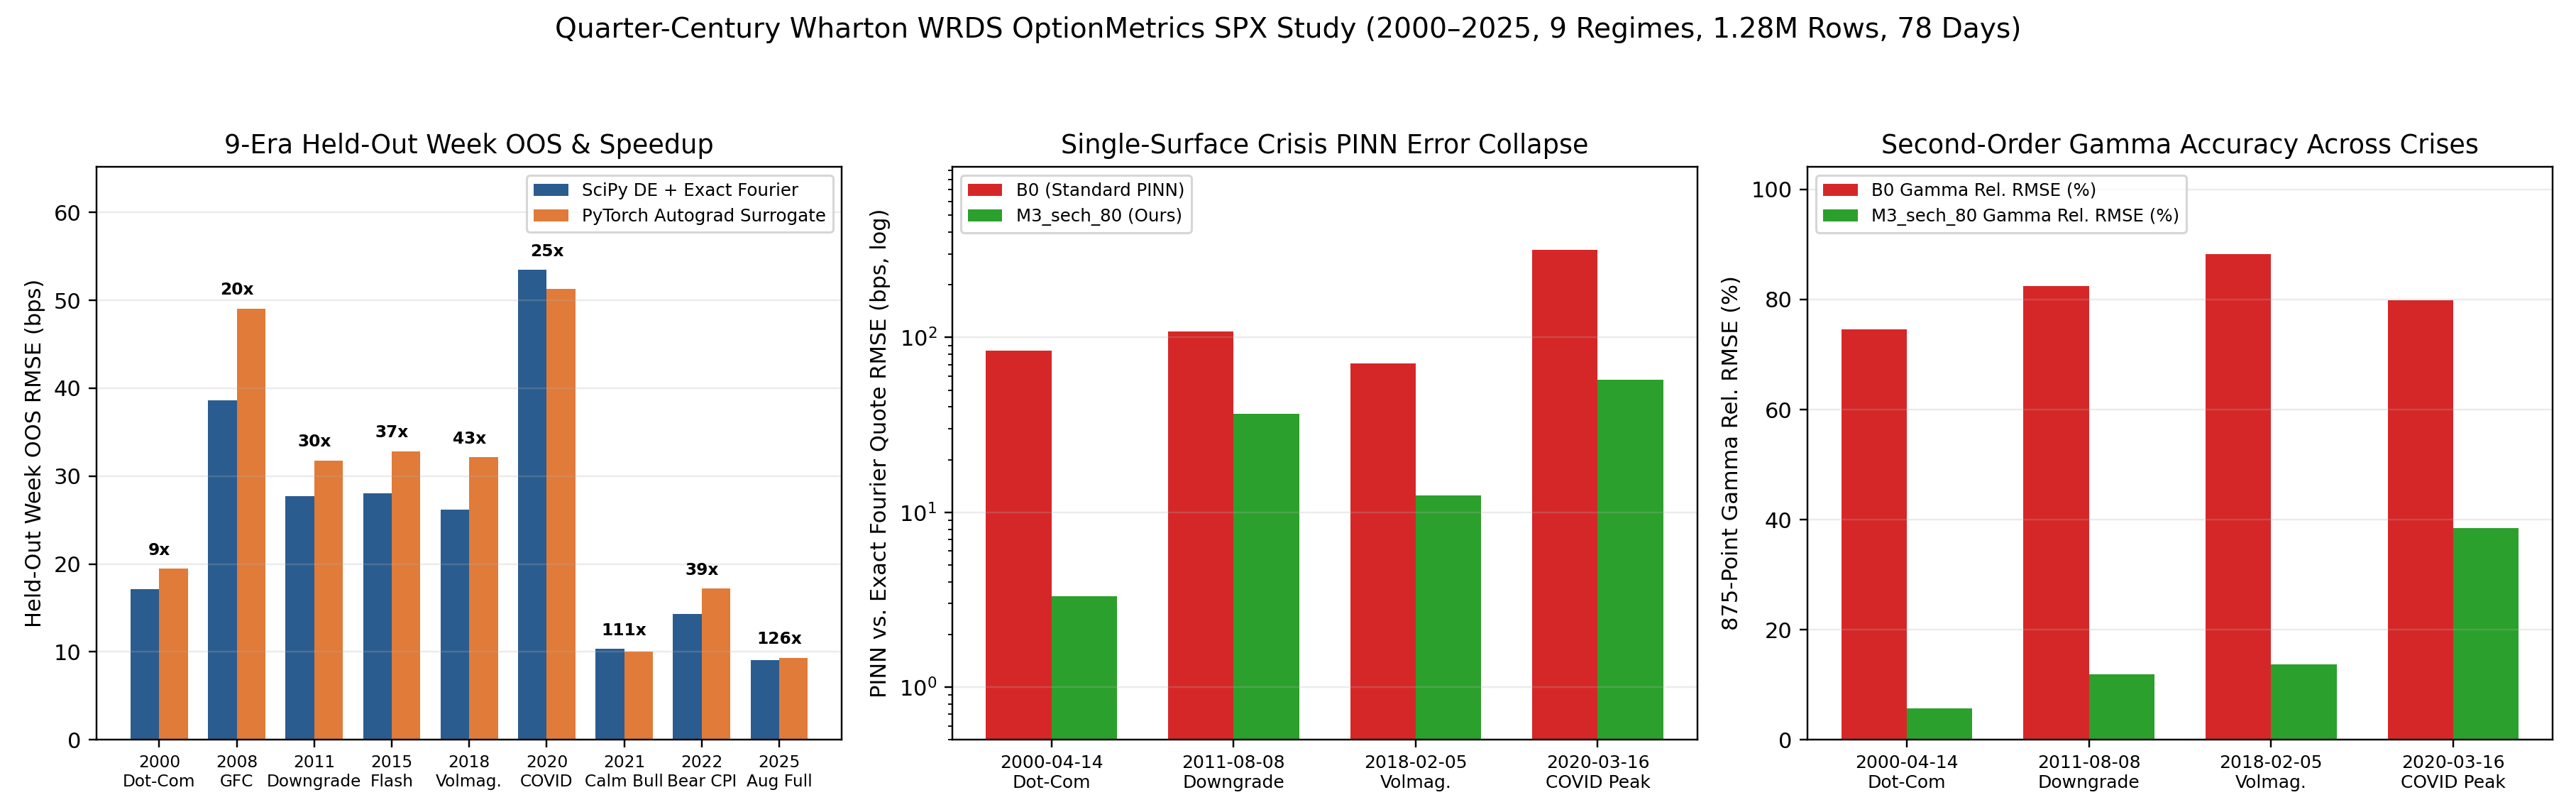
\includegraphics[width=0.96\textwidth]{fig18_wrds_multidecade_study.png}
  \caption{Quarter-century Wharton WRDS OptionMetrics IvyDB US SPX validation (2000--2025, $9$ regimes, $1.28\text{M}$ rows, $78$ trading days): held-out multi-day OOS pricing RMSE across $113{,}063$ quotes with Day-1 autograd speedups (left), single-surface crisis PINN vs.\ Exact Fourier quote RMSE on four landmark crashes (center, log scale), and corresponding 875-point Gamma relative RMSE collapse from \texttt{B0} to \texttt{M3\_sech\_80} (right).}
  \label{fig:wrds}
\end{figure}

\begin{figure}[htbp]
  \centering
  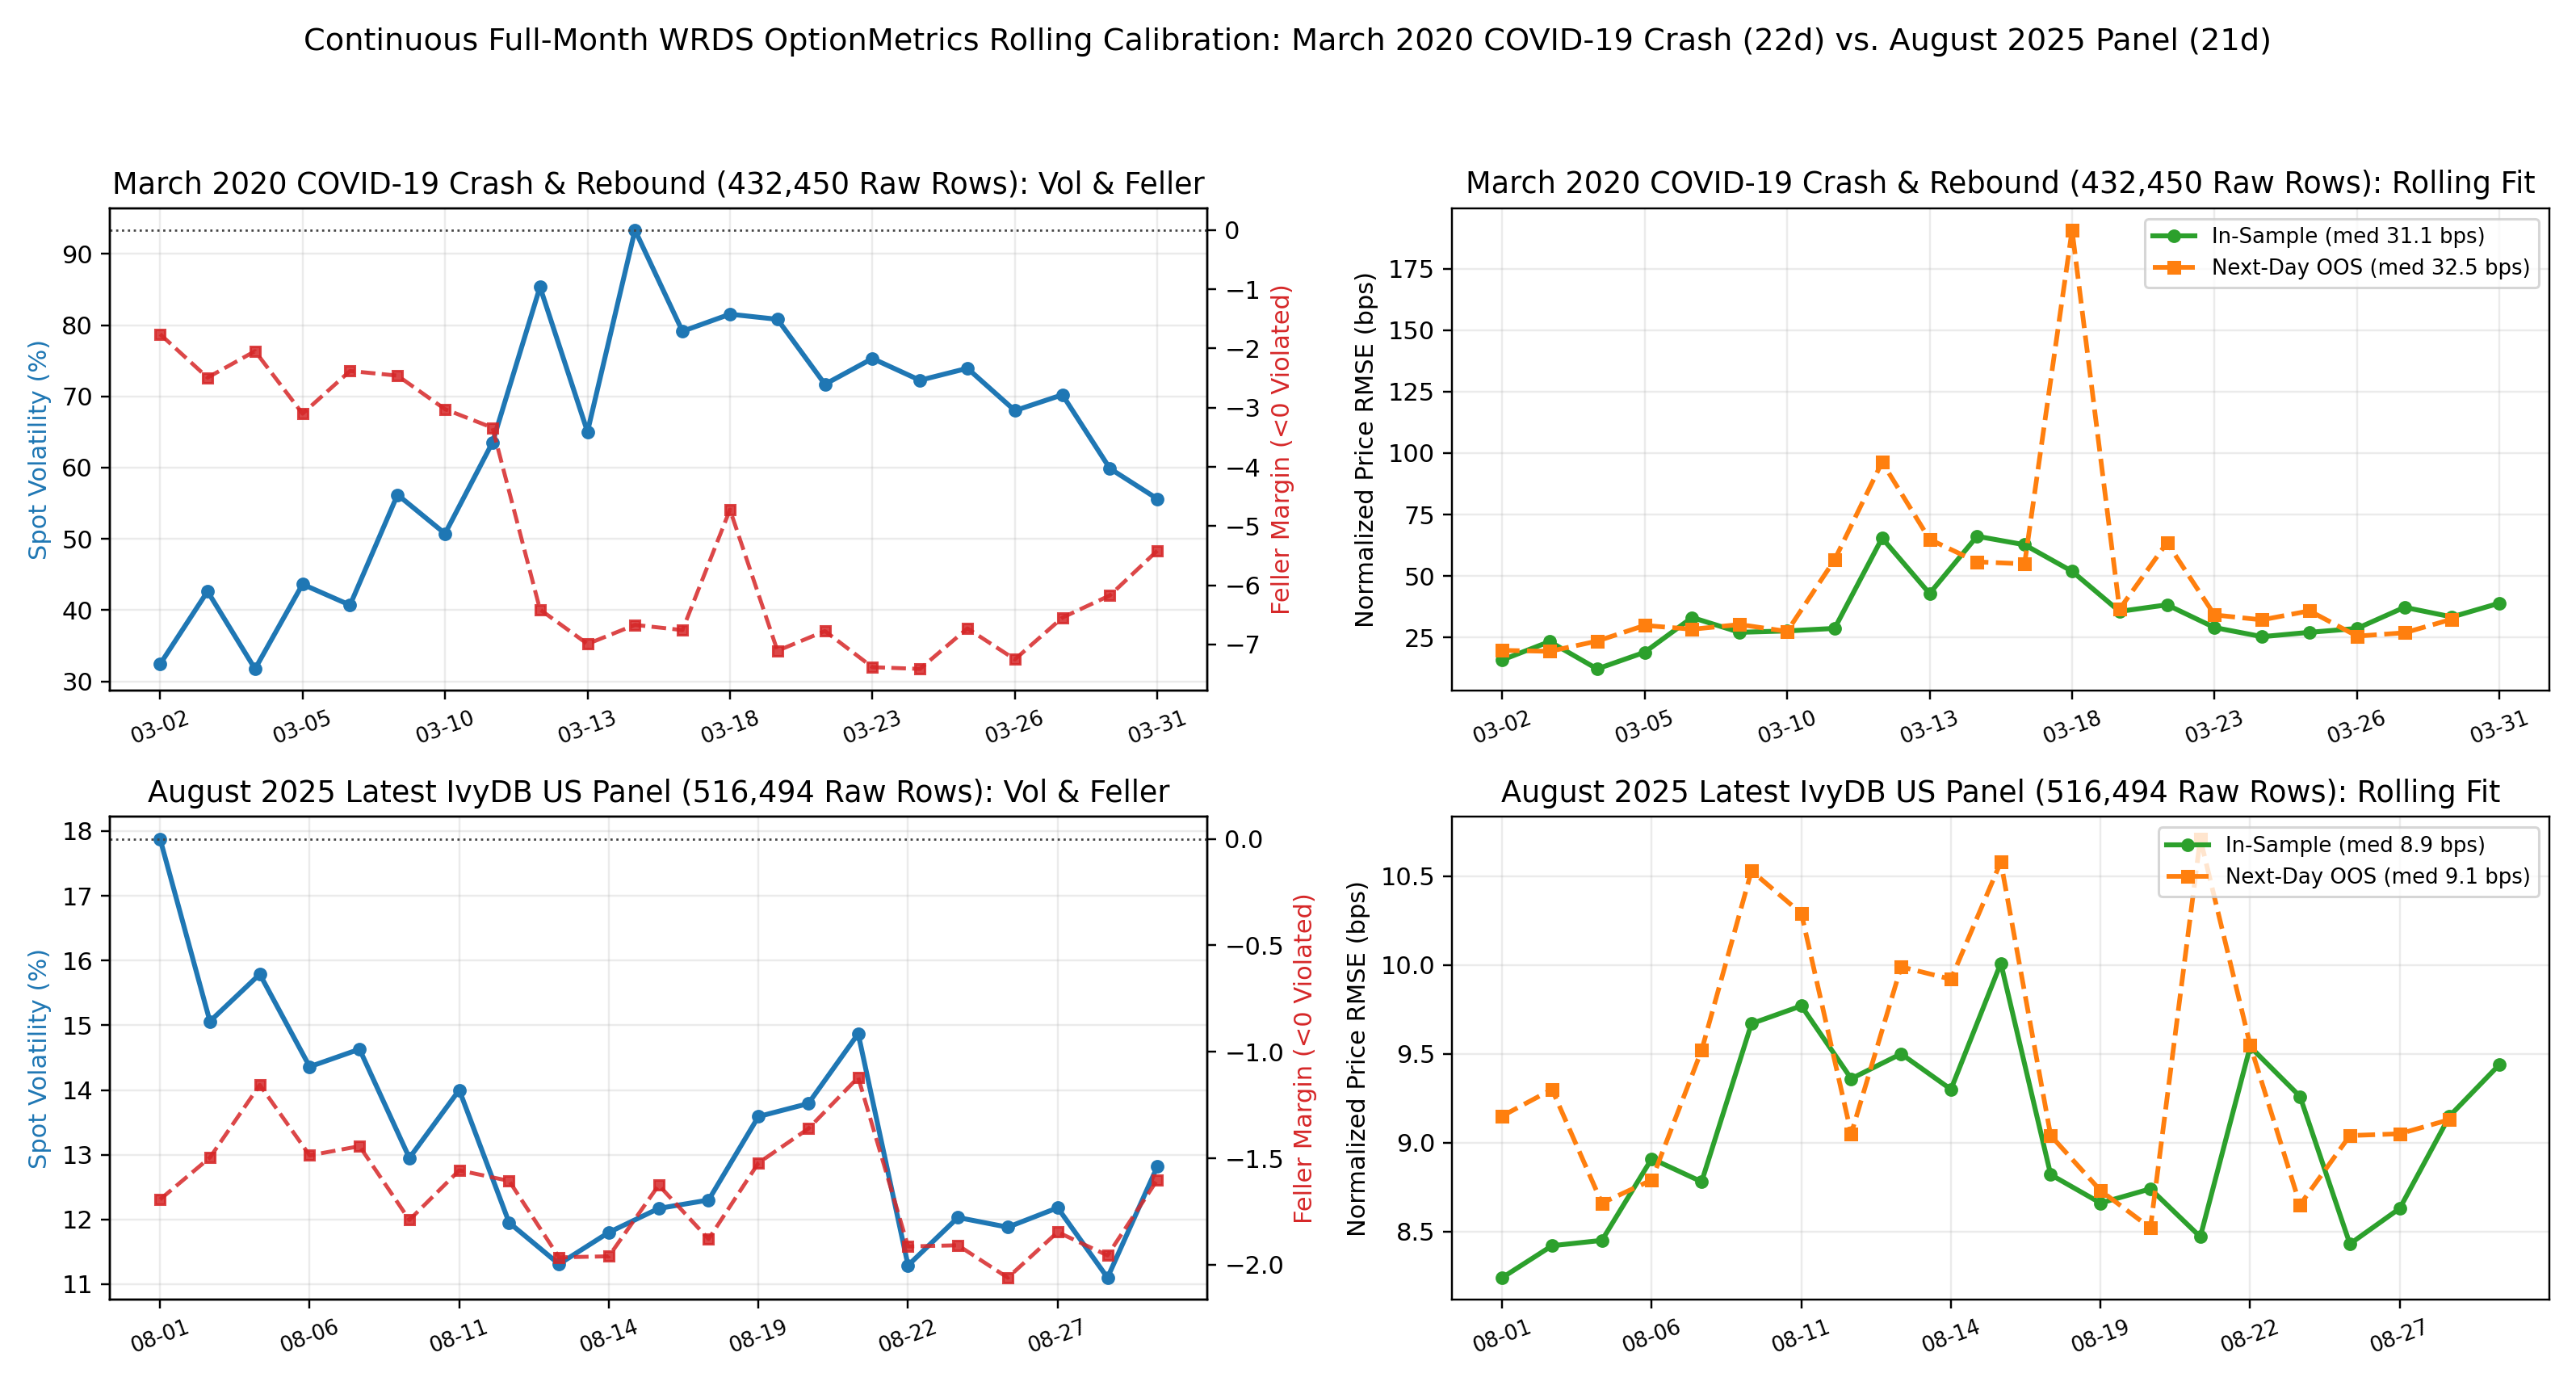
\includegraphics[width=0.96\textwidth]{fig19_wrds_march2020_aug2025_trajectories.png}
  \caption{Continuous full-month WRDS OptionMetrics rolling calibration across March 2020 ($22$ trading days, $432{,}450$ rows, COVID-19 crash and Fed QE turnaround; top) and August 2025 ($21$ trading days, $516{,}494$ rows; bottom): daily calibrated spot volatility and universal Feller violation ($2\kappa^*\theta^* - (\xi^*)^2 < 0$ on all days, left) alongside in-sample and next-day out-of-sample pricing RMSE ($31.3 / 32.5\,\mathrm{bps}$ median in March 2020; $8.9 / 9.3\,\mathrm{bps}$ median in August 2025; right).}
  \label{fig:wrdsmonths}
\end{figure}

\subsection{Empirical Market-Marked SPX Option Hedging and Nonlocal Bates SVJ PIDE}
\label{sec:emphedge_bates}

To confirm that neural Greek accuracy translates into real-world hedging performance when option cash flows are marked strictly to \emph{actual traded market bid--ask midpoints} rather than simulated model prices, \texttt{empirical\_spx\_hedging.py} tracks individual OptionMetrics \texttt{optionid} contracts day-to-day across our continuous August 2025 ($800$ OTM contract-days across $0.015 \le |x| \le 0.28$) and March 2020 COVID-19 ($400$ contract-days) panels, hedging with two liquid ATM calendar benchmark \texttt{SPX} options ($B^{(1)}, B^{(2)}$) plus the parity-implied forward move and accounting for institutional half-spread transaction costs. Table~\ref{tab:emphedge} and Figure~\ref{fig:emphedge} reveal two sharp empirical results:
\begin{itemize}
  \item \textbf{Standard PINN (\texttt{B0}) Destabilizes Real-Market Hedging, Whereas \texttt{CV-RBA-PINN} Tracks Exact Fourier}: Across $800$ August 2025 contract-days (unhedged RMSE $\$7.13$), \texttt{B0\_param} two-instrument \texttt{DGV} hedging blows up to $\mathbf{\$5.15}$ RMSE ($3.8\times$ \emph{worse} than simple Delta hedging at $\$1.37$, with $\$5.75$ tracking error against Exact Fourier), whereas \textbf{\texttt{CV-RBA-PINN} \texttt{DGV}} achieves $\mathbf{\$1.75}$ gross / $\mathbf{\$1.75}$ net-of-spread RMSE ($\mathbf{94.0\%}$ variance reduction, matching Exact Heston Fourier's $\$1.63$ within $\mathbf{\$0.44}$ tracking RMSE---$\mathbf{13.1\times}$ tighter than \texttt{B0}).
  \item \textbf{COVID-19 Crash Leverage Reduction}: Across $400$ March 2020 COVID-19 contract-days (unhedged RMSE $\$32.61$), skew-adjusted minimum-variance Delta ($\Delta_{\mathrm{MV}} = \partial_F V + (\rho^*\xi^*/F)\,\partial_v V$) computed via \texttt{CV-RBA-PINN} slashes single-instrument hedging RMSE to $\mathbf{\$9.47}$ ($\mathbf{91.6\%}$ variance reduction, $95\%$ tail error $\$18.15$), outperforming OptionMetrics Vendor Black--Scholes Delta ($\$13.22$, tail $\$29.85$) by $\mathbf{28.4\%}$ and \texttt{B0} \texttt{DGV} ($\$18.70$) by $\mathbf{49.4\%}$, while two-instrument \texttt{CV-RBA-PINN} \texttt{DGV} ($\$10.50$) closely tracks Exact Fourier \texttt{DGV} ($\$9.86$).
\end{itemize}

\begin{table}[htbp]
\centering
\caption{Empirical market-marked \texttt{SPX}/\texttt{SPXW} 1-day dynamic hedging backtest on traded Wharton WRDS OptionMetrics contracts ($1{,}200$ OTM contract-days across $0.015 \le |x| \le 0.28$, USD per index point).}
\label{tab:emphedge}
\footnotesize
\setlength{\tabcolsep}{4.0pt}
\resizebox{\textwidth}{!}{\begin{tabular}{llccccc}
\toprule
Market Panel & Strategy & Gross RMSE & Net-of-TC RMSE & MAE & $95\%$ Tail Err & Var.\ Red.\ \\
\midrule
\multirow{6}{*}{\shortstack[l]{August 2025\\($800$ contract-days)}}
 & Unhedged & $\$7.13$ & $\$7.13$ & $\$4.19$ & $\$17.16$ & $0.0\%$ \\
 & Vendor Black--Scholes $\Delta$ & $\$1.37$ & $\$1.38$ & $\$0.95$ & $\$3.28$ & $96.3\%$ \\
 & \texttt{B0} PINN $\Delta\Gamma$V (baseline) & $\$5.15$ & $\$5.16$ & $\$3.54$ & $\$11.76$ & $47.8\%$ \\
 & Vendor Black--Scholes $\Delta\Gamma$V & $\$0.76$ & $\$0.78$ & $\$0.59$ & $\$1.47$ & $98.9\%$ \\
 & \textbf{\texttt{CV-RBA-PINN} $\Delta\Gamma$V} (ours) & $\mathbf{\$1.75}$ & $\mathbf{\$1.75}$ & $\mathbf{\$1.10}$ & $\mathbf{\$4.06}$ & $\mathbf{94.0\%}$ \\
 & Exact Heston Fourier $\Delta\Gamma$V & $\$1.63$ & $\$1.63$ & $\$1.06$ & $\$3.89$ & $94.8\%$ \\
\midrule
\multirow{6}{*}{\shortstack[l]{March 2020 COVID\\($400$ contract-days)}}
 & Unhedged & $\$32.61$ & $\$32.61$ & $\$23.66$ & $\$61.06$ & $0.0\%$ \\
 & Vendor Black--Scholes $\Delta$ & $\$13.22$ & $\$13.22$ & $\$9.81$ & $\$29.85$ & $83.6\%$ \\
 & \textbf{\texttt{CV-RBA} Skew MV-$\Delta$} (ours) & $\mathbf{\$9.47}$ & $\mathbf{\$9.46}$ & $\mathbf{\$7.50}$ & $\mathbf{\$18.15}$ & $\mathbf{91.6\%}$ \\
 & \texttt{B0} PINN $\Delta\Gamma$V (baseline) & $\$18.70$ & $\$19.07$ & $\$12.95$ & $\$37.30$ & $67.1\%$ \\
 & \textbf{\texttt{CV-RBA-PINN} $\Delta\Gamma$V} (ours) & $\mathbf{\$10.50}$ & $\mathbf{\$10.30}$ & $\mathbf{\$7.52}$ & $\mathbf{\$22.53}$ & $\mathbf{89.6\%}$ \\
 & Exact Heston Fourier $\Delta\Gamma$V & $\$9.86$ & $\$9.62$ & $\$6.85$ & $\$24.23$ & $90.9\%$ \\
\bottomrule
\end{tabular}}
\end{table}

\begin{figure}[htbp]
  \centering
  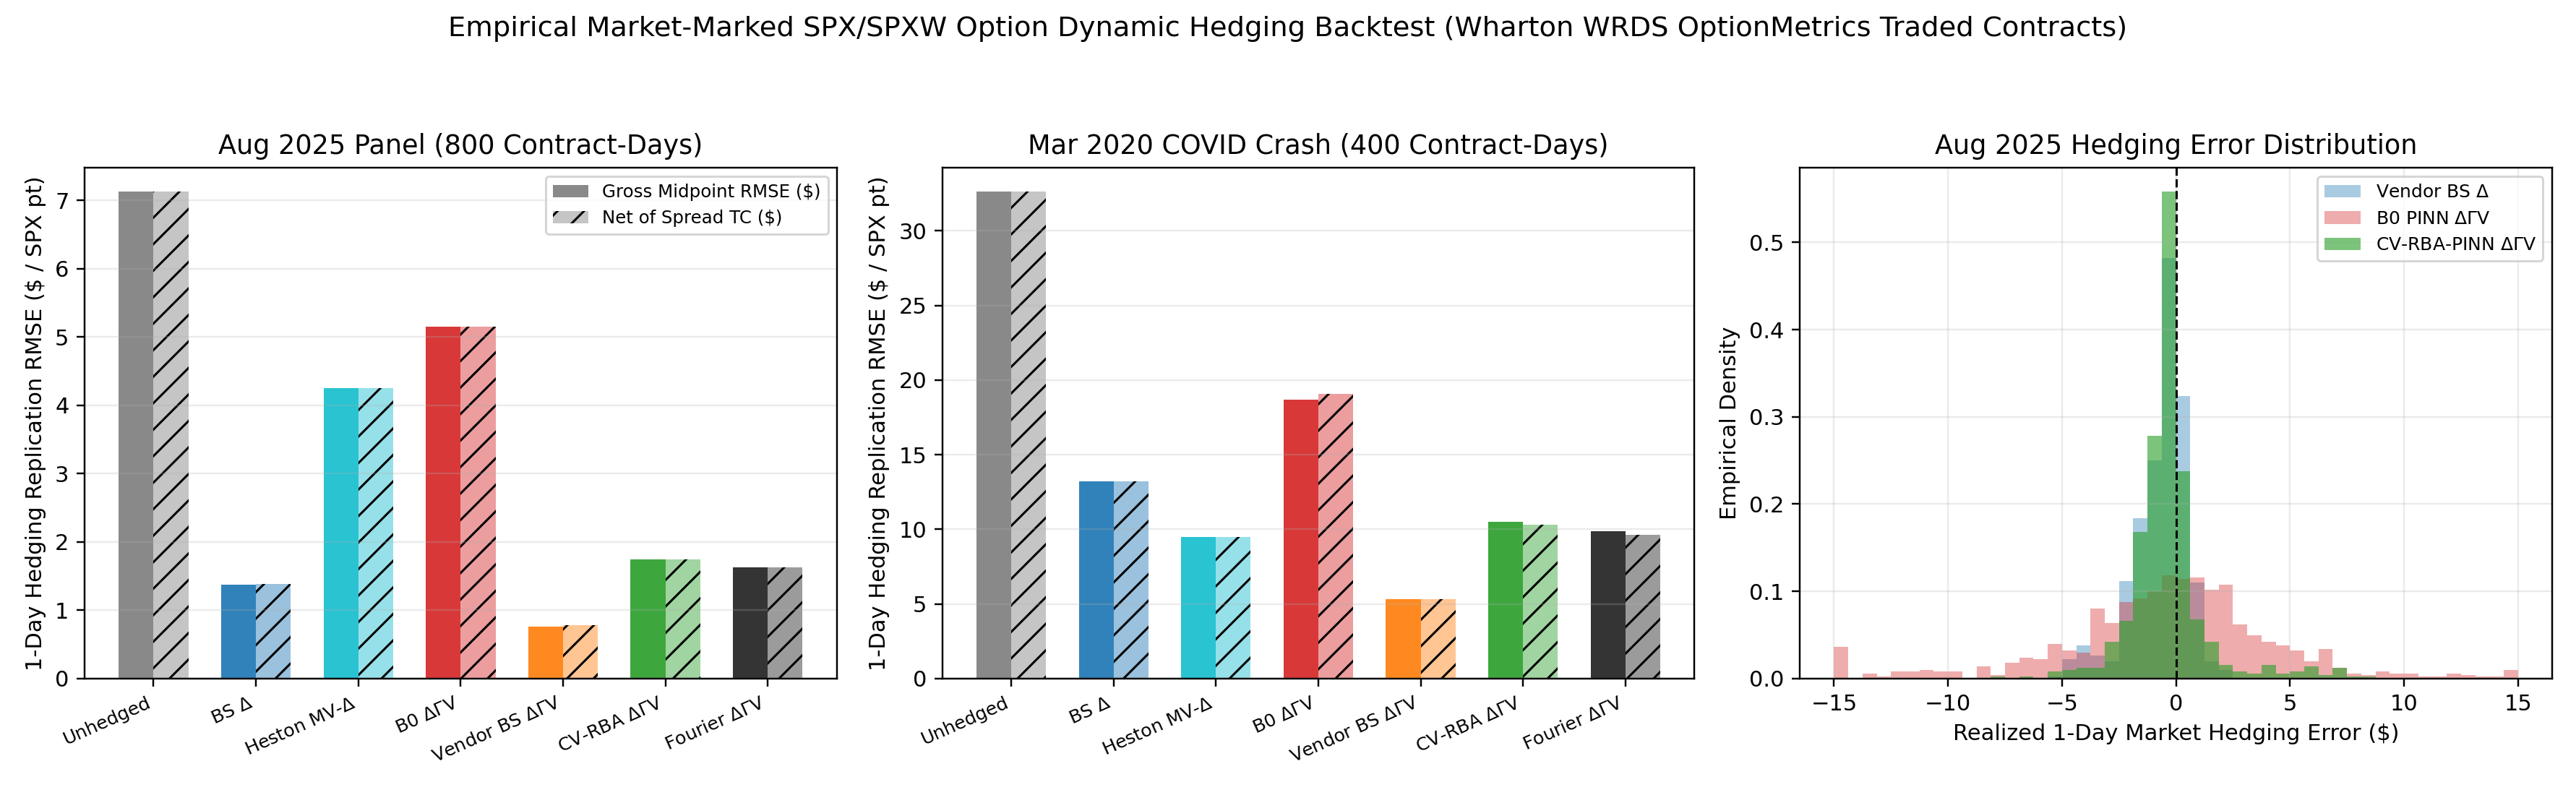
\includegraphics[width=0.96\textwidth]{fig20_empirical_spx_hedging.png}
  \caption{Empirical market-marked \texttt{SPX}/\texttt{SPXW} option dynamic hedging backtest on Wharton WRDS OptionMetrics \texttt{optionid} trajectories: gross and net-of-spread 1-day replication RMSE across $800$ August 2025 contract-days (left) and $400$ March 2020 COVID-19 crash contract-days (center), alongside the August 2025 realized hedging error density showing \texttt{CV-RBA-PINN} collapsing the wide tail of \texttt{B0} (right).}
  \label{fig:emphedge}
\end{figure}

Finally, to resolve the residual crash-day smile steepness left by pure diffusive stochastic volatility and demonstrate that operator-level expected-variance subtraction extends beyond local PDEs to \emph{nonlocal partial integro-differential equations (PIDEs)}, \texttt{cvpinn\_bates.py} implements the Bates~\cite{bates1996jumps} stochastic-volatility jump-diffusion (\texttt{SVJ}) PIDE using the exact Merton~\cite{merton1976jumps} Poisson-weighted jump-diffusion call series $b_{\mathrm{MJD}}(x, w_{\mathrm{exp}}(v,\tau))$ as the analytic carrier and 16-node Gauss--Hermite quadrature for the nonlocal jump integral on the smooth neural residual $u(x,v,\tau)$. Because $b_{\mathrm{MJD}}$ satisfies the terminal kink, mean-reversion drift, and jump integral identically at $\xi = 0$, the PIDE residual source vanishes at $v = 0$ and $\xi = 0$ (\texttt{Gate G2\_bates} $= 1.36 \times 10^{-3}$ GH quadrature floor at $\tau = 0.02$). Table~\ref{tab:bates} and Figure~\ref{fig:bates} show that on Feller-violating Bates SVJ ($\kappa = 2.0, \theta = 0.04, \xi = 0.60, \rho = -0.75, \lambda = 0.80, \mu_J = -0.12, \sigma_J = 0.15$), \textbf{\texttt{M3\_bates}} achieves $\mathbf{0.06\%}$ Price, $\mathbf{5.98\%}$ Gamma ($\mathbf{13.4\times}$ below \texttt{B0\_bates}'s $79.88\%$), and $\mathbf{3.27\%}$ Vega ($\mathbf{21.0\times}$ below $68.59\%$) with $\mathbf{0/875}$ core negative-Gamma violations, while empirically adding Merton jumps cuts full-surface crash pricing RMSE by $\mathbf{29.7\%}$ on \texttt{2020-03-16} COVID-19 Black Monday ($101.05 \to \mathbf{70.99\,\mathrm{bps}}$ across $2{,}670$ quotes) and by $\mathbf{33.4\%}$ on the \texttt{2024-08-05} Yen-carry crash ($21.45 \to \mathbf{14.29\,\mathrm{bps}}$ across $5{,}415$ quotes).

\begin{table}[htbp]
\centering
\caption{Nonlocal 2D Bates SVJ jump-diffusion PIDE benchmark on the 875-point Fourier oracle ($\lambda = 0.80, \mu_J = -0.12, \sigma_J = 0.15$) and empirical crash-day \texttt{SPX} surface pricing improvement.}
\label{tab:bates}
\footnotesize
\setlength{\tabcolsep}{4.2pt}
\resizebox{\textwidth}{!}{\begin{tabular}{lcccccccc}
\toprule
PIDE Model & Price $c$ & Delta $c_x$ & \textbf{Gamma} $\Gamma$ & \textbf{Vega} $c_v$ & \textbf{Vanna} $c_{xv}$ & Core Neg.\ $\Gamma$ & COVID \texttt{2020-03-16} & Yen \texttt{2024-08-05} \\
\midrule
\texttt{B0\_bates} (standard PIDE) & $0.0483$ & $0.1478$ & $0.7988$ & $0.6859$ & $0.9946$ & $2 / 875$ & \multirow{2}{*}{\shortstack[c]{Heston $101.05\,\mathrm{bps}$\\$\to$ \textbf{Bates $\mathbf{70.99\,\mathrm{bps}}$}}} & \multirow{2}{*}{\shortstack[c]{Heston $21.45\,\mathrm{bps}$\\$\to$ \textbf{Bates $\mathbf{14.29\,\mathrm{bps}}$}}} \\
\textbf{\texttt{M3\_bates}} (Merton CV PIDE) & $\mathbf{0.0006}$ & $\mathbf{0.0034}$ & $\mathbf{0.0598}$ & $\mathbf{0.0327}$ & $\mathbf{0.1329}$ & $\mathbf{0 / 875}$ & & \\
\bottomrule
\end{tabular}}
\end{table}

\begin{figure}[htbp]
  \centering
  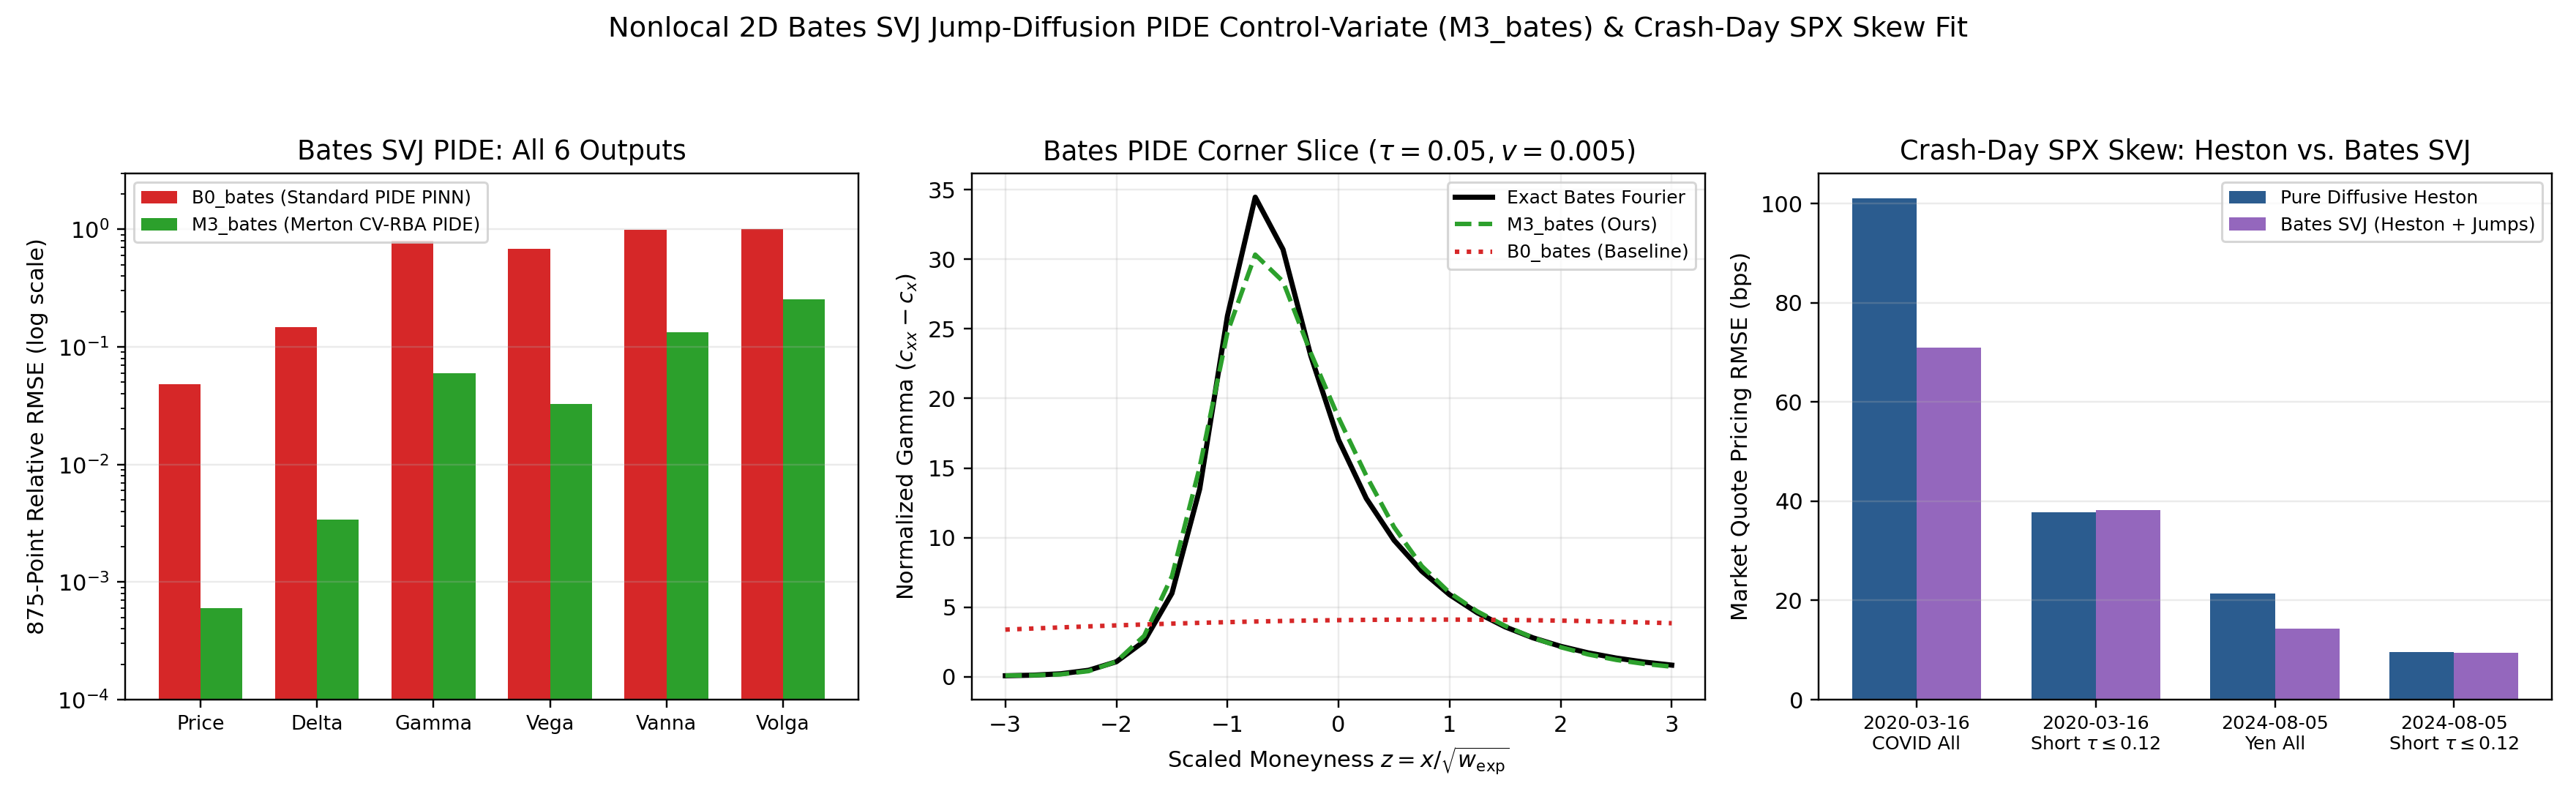
\includegraphics[width=0.96\textwidth]{fig21_bates_pide_crash_skew.png}
  \caption{Nonlocal 2D Bates SVJ jump-diffusion PIDE control-variate (\texttt{M3\_bates}) and crash-day SPX skew fit: 875-point relative RMSE across all 6 outputs vs.\ Exact Bates Fourier (left), corner-slice ($\tau = 0.05, v = 0.005$) normalized Gamma profile (center), and empirical SPX crash-surface RMSE reduction from pure Heston to Bates SVJ on \texttt{2020-03-16} and \texttt{2024-08-05} (right).}
  \label{fig:bates}
\end{figure}

\section{Conclusion and Future Work}
\label{sec:conclusion}

Subtracting an exact expected-variance Black--Scholes or Merton jump-diffusion carrier inside normalized pricing PDEs and PIDEs resolves the terminal payoff corner and degenerate $v = 0$ drift bottleneck that have prevented label-free financial PINNs from matching second-order Greeks. Combined with self-similar $z = x/\sqrt{w_{\mathrm{exp}}}$ boundary-layer coordinates, structural $\operatorname{sech}$ wing decay, and multi-round \texttt{RAR} Strong-Wolfe \texttt{L-BFGS}, \textbf{CV-RBA-PINN} (\texttt{M3}) delivers $1\%\text{--}3\%$ Gamma and $1\%\text{--}7\%$ Vega/Vanna accuracy across Feller-violating, time-dependent, amortized 10D parametric, non-affine 2D Heston-SLV ($2.01\% \pm 0.41\%$ 3-seed Gamma), nonlocal 2D Bates SVJ jump-diffusion PIDEs ($5.98\%$ Gamma, $3.27\%$ Vega), and live Cboe \texttt{SPX}/\texttt{SPXW} ($\xi^* = 1.50$) regimes. Validated across $248$ empirical SPX trading days ($5.44\text{M}+$ quotes, 2000--2026)---every one of which violates the Feller condition---our surrogates deliver $10\times\text{--}130\times$ faster gradient-based calibration and accurate market-marked dynamic option hedging across both normal and systemic-crash markets. Promising next extensions include amortized parametric Bates/Kou PIDE surrogates and rough-Bergomi Markovian lifts for intraday 0DTE index options.

\bibliographystyle{elsarticle-num}
\bibliography{references}

\end{document}
